% UICTEST.TEX
% This is a test file for my port of UICTHESI
% to LaTeX 2e. This is based in part on UCTHESIS.
%

%\documentclass[draft]{uicthesi}
\documentclass{uicthesi}
\usepackage{tabularx} %vita
\usepackage{ltablex} % for pagebreaks of tabularx
\usepackage{array}		 %vita
\usepackage{longtable} %vita
\usepackage{ltxtable}  %vita 
\usepackage{siunitx}
\usepackage{xfrac}
\usepackage[english]{babel}
\usepackage{mwe}
\usepackage{graphicx}
\usepackage{subfigure}
\usepackage[colorinlistoftodos]{todonotes}
\usepackage{amsmath}
\usepackage{algorithm2e}
\usepackage{pdfpages}
\usepackage{enumerate}
\usepackage{amsfonts}
\usepackage{caption} 
\usepackage{url}
\usepackage{hyperref}
\usepackage{listings}
\usepackage{color}
\usepackage{multirow}
\usepackage[export]{adjustbox}

% Define code colors
\definecolor{codegreen}{rgb}{0,0.6,0}
\definecolor{codegray}{rgb}{0.5,0.5,0.5}
\definecolor{codepurple}{rgb}{0.58,0,0.82}
\definecolor{backcolour}{rgb}{0.95,0.95,0.92}
 
\lstdefinelanguage{NutellaProtocol}{
  keywords={id, from, type, payload, run_id, app_id, component_id, resource_id},
  keywordstyle=\color{codepurple}\bfseries,
  ndkeywords={run, request},
  ndkeywordstyle=\color{orange}\bfseries,
  identifierstyle=\color{codegray},
  sensitive=false,
  comment=[l]{//},
  morecomment=[s]{/*}{*/},
  commentstyle=\color{codegreen}\ttfamily,
  % stringstyle=\color{black}\ttfamily
}

\lstset{
   language=NutellaProtocol,
   backgroundcolor=\color{white},
   extendedchars=true,
   basicstyle=\linespread{1.5}\footnotesize\ttfamily,
   showstringspaces=false,
   showspaces=false,
   tabsize=2,
   breaklines=true,
   showtabs=false,
   captionpos=b
}
\begin{document}

% Declarations for Front Matter

\title{RoomPlaces: a system for supporting science inquiry in the Classroom of Things}
\author{Gianluca Venturini}
\pdegrees{B.S, Politecnico di Milano, Milan, Italy, 2015}
\degree{Master in Computer Science}
\maketitle


\acknowledgements
{Firstly, I would like to express my sincere gratitude to my advisor Prof. Tom Moher for the continuous support of my Master study and related research, for his patience, motivation, and immense knowledge. His guidance helped me in all the time of research and writing of this thesis. I could not have imagined having a better advisor and mentor for my Master study.\\

Besides my advisor, I would like to thank the rest of my thesis committee: Prof. Ugo Buy and Prof. Franca Garzotto for their insightful comments and encouragement.\\

I thank my fellow labmates and friends at the Learning Technologies Group for the stimulating discussions, for the sleepless nights we were working together before deadlines, and for all the fun we have had in the last year.\\

Finally, I would like to thank my friends and my family: my parents and my sister for supporting me spiritually throughout writing this thesis and my life in general.

\begin{flushright}
GV %(your initials)
\end{flushright}}


\tableofcontents
\listoftables
\listoffigures
\listofabbreviations
\begin{list}
{}
{\setlength
   {\labelwidth}{1in}
    \setlength{\leftmargin}{1.5in}
    \setlength{\labelsep}{.5in}
    \setlength{\rightmargin}{\leftmargin}}
\item[API\hfill] Application programming interface
\item[DBm\hfill] Becibel milliwatt
\item[FM\hfill] Frequency Modulation
\item[GPS\hfill] Global Positioning System
\item[JSON\hfill] JavaScript Object Notation
\item[KCI\hfill] Knowledge  Community  and  Inquiry
\item[LED\hfill] Light Emitting Diode
\item[MQTT\hfill] MQ Telemetry Transport
\item[PDA\hfill] Personal Digital Assistant
\item[PIC\hfill] Peripheral Interface Controller
\item[RFID\hfill] Radio-Frequency IDentification
\item[RID\hfill] Resource Identifier
\item[TCP\hfill] Transmission Control Protocol
\item[TUI\hfill] Tangible User Interfaces
\item[UIC\hfill] University of Illinois at Chicago
\item[USB\hfill] Universal Serial Bus
\end{list}

\squarebrackets %this makes the citations with square brackets
\captionsetup[table]{skip=10pt} %to separate table captions from the table itself

\summary

\label{chap:summary}

This thesis offers two distinct and complementary contributions. First, it introduces a software framework called RoomPlaces that supports proximity location tracking of students and artifacts in classrooms using Bluetooth Low Energy beacon technology. RoomPlaces provides a set of functions that allow developers to both query the system for the location of an object and subscribe to notifications of arrival and departure events from discrete locations. While these capabilities could be used to support a variety of services such as automatic attendance, inventory management, and monitoring of resource utilization, the focus here is on the use of the location as a driver for scientific simulation. 

Second, RoomPlaces is used to support an exploratory study conducted on the embedded phenomena WallCology (Moher, et al., 2008), where the location of shared tangible artifacts is used to control a distributed simulation of ecosystem dynamics. Students are required to work in groups with the goal of discovering the dynamics of the interactions among species situated inside simulated ecosystems. Students have the capability to alter the species composition and population levels present in those virtual environments and observe how they respond to uncontrollable external pressures such as warming, habitat destruction, and the invasion of alien species.

Research in community knowledge construction has shown that getting students to seek and share information with one another is extremely challenging. Students in three sixth-grade classes were provided with a single set of shared control artifacts with embedded Bluetooth LE beacons, creating a bottleneck designed to promote interaction and information sharing among groups. We present evidence supporting the claim that the use of the tangibles raised learners' motivation to participate in the activity, fostered productive disciplinary discourse, and heightened student sense of autonomy and control during the activity.

\chapter{Introduction}

\label{chap:introduction}

In the last two decades the development of new computing technologies has radically expanded and became pervasive in every aspect of our life. Those technologies are transforming and expanding the activity structures that can be designed and built for school classrooms with the goal of supporting students and teachers during the process of learning. The \textit{Classrooms of Things} is becoming a reality: more and more computing artifacts are created and connected to the network with the goal of teaching a particular concept. It is important to understand the implications of this technology and to explore how can we take advantage of it for creating the classroom activities of the future. The vision is building cheap and easy to use applications that can be purchased, configured and ran by school teachers that will be in full control of the whole class activity customizing it for the needs of the students.

Past researches in the field of learning sciences highlighted the opportunity of creating a system that address the needs of using objects as interface for interacting with computing devices. In this thesis I explore how to take advantage of this opportunity for integrating embodied and tangible interactions inside a large variety of activities that involve the whole classroom. There are mainly two trends that take a different approach in order to enhance the excitement and stimulate the process of learning through hands-on activities: \textit{embodiment} and \textit{tangibles}. In embodiment the movement of the whole body is used as a way for interacting with the system: it is based on different body metaphors associating different movements and gestures with different concepts that have to be teached. Tangibles are physical objects used for interacting with virtual environments. They can be used as input devices or as computing systems themselves.

\section{Whole body movement}
With the term \textit{embodiment} I mean the enactment of knowledge and concepts though the activities of the whole body. The activities based on that are considered from the learning science community to have a strong potential to engage learners in immersive experiences that enhance their education \cite{lindgren:emboldened}. It is based on the simple idea that human cognition is deeply rooted in the body’s interactions with its physical environment. There are increasing evidence that body movements (for example gestures) can facilitate the retrieval of mental and lexical items. That’s because cognitive processes involved in learning (e.g. conceptual development and comprehension) are built upon a foundation of physical embodiment. When the right sensorimotor systems are engaged a stronger and persistent knowledge representation is created \cite{lindgren:emboldened} and for this reason the authors believe that learning activities involving embodiment lead to a greater chance of retrieval and retention of this information.

In order to implement this idea inside classroom activities different research teams developed different formats. \textit{Mixed Reality} is a term describing the space in between entirely real-world environments and entirely virtual environments  \cite{milgram:taxonomy} where computational devices are used in order to augment the physical reality, in other words activities that are conducted in the physical space of the class with the help of computer simulations and different interfaces for interacting with it. Mixed Reality can take a number of forms such digital overlays on real world scenes, for example projections on walls, floors and other surfaces. Evidence suggests that this format supports productive social interactions and a generates a positive atmosphere of playfulness and experimentation. A very important concept introduced in this framework is the \textit{body-based metaphors} that enable to translate natural movements of the user body into a behavior of virtual elements \cite{lindgren:supporting}. If the metaphor holds than the simulation responds in a way that is consistent with the child’s intuitive movements and gives feedback that enable immediate learning by doing.

Many elements of Mixed Reality can be found in the work made by Colella \cite{colella:virus} describing \textit{Participatory Simulations} as a way for plunging learners into life-sized, computer-supported simulations where the user acts as a component (an actor) of the simulation. \textit{Simulated investigations} on the other end are developed with the same principles of \textit{Mixed Reality}, but this time the user plays the role of the scientist developing theories about dynamic systems. The student is the observer (doesn't take part in the simulation) and the technology play a supporting role for the scientific research that is conducted. \textit{Embedded Phenomena} is a learning technology framework in which simulated scientific phenomena are mapped onto the physical space of classrooms \cite{moher:embedded} and continue over a long period of time: two to three months in which the investigated phenomena evolves overtime.

\subsection{Participatory Simulations}
\textit{Participatory Simulations} is a term introduced by Colella \cite{colella:virus} and describes a new set of activities that immerse the students inside the phenomena itself by transforming them in elements of it (e.g. a bee \cite{peppler:beesim}, an infected individual \cite{colella:virus} and a squirrel foraging for food \cite{gnoli:hunger_games}). Sensor based devices are carried or worn by participants (e.g. \textit{Thinking Tags} \cite{colella:virus}, GPS enabled handheld devices) and they allow exchange of contextually relevant information. Participants experience the simulations in many different ways: at local level (from the perspective of the element that they are impersonating), global level where they can see how actions of other individuals affect patterns within the overall system and from outside (e.g. after the simulation ends, students look at the collected data and try to explain the phenomena). Technology is mainly used in order to support the game with all the rules and the possible interactions. Examples of participatory simulations are: BeeSim \cite{peppler:beesim}, Hunger Games \cite{gnoli:hunger_games}, Virus Simulation \cite{colella:virus} and Savannah \cite{facer:savannah} and they are explained in details in the next chapter.

\subsection{Simulated investigations}
In \textit{Simulated Investigations} the student assumes the role of a scientist and the main focus is on the studied phenomena. The role of the technology is simulating the phenomena, helping the user during the inquiry with tools that resemble the real ones, supporting findings and helping documenting facts and discoveries. Another interesting characteristic is that those simulations last for many weeks in which students can gather and aggregate evidence to answer questions related to the object of inquiry.

\subsection {Embedded Phenomena}
Embedded Phenomena term was created by Moher \cite{moher:embedded} and describes a simulated scientific investigation about certain phenomena that is mapped inside the physical space of the classroom. It intends to create opportunities for students to explore a certain scientific domain with the goal of gathering as many information as they can in order to answer questions and learning the specific lexis about the topic during an extended period of observation (that usually is few months). The fundamental element of every embedded phenomena is the mapping between different part of the phenomena inside the physical space of the classroom. The second element is the state of the simulation that is represented though different media, distributed around the classroom representing portals into that phenomenon. The simulations are persistent and their state is observable in every moment during the whole period of time. The state can also be manipulated though different interfaces and the students can use manipulations for collectively gather evidence to answer a questions and solve problems. 

This framework represents the perfect opportunity for testing how objects became a component of the simulation and what are the characteristics that they must have for producing real learning advantages. In the user study described in \autoref{chap:user_study} tangible objects are integrated inside \textit{WallCology} Embedded Phenomena \cite{moher:wallcology}.

\subsection{Macroworlds}

A successive evolution of Embedded Phenomena are the Macroworlds that are technology-enhanced learning environments that leverage the notions of ubiquitous computing introduced by Weiser \cite{weiser:computer} and the distributed interaction \cite{luyten:distributed} to provide engaging ways for students to experience and interact with classroom sized scientific phenomena. Fundamental capability for a \textit{Macroworld} is the tracking of object movements inside a room in order to use it as an interface between the user and the simulation that is running inside the computing environment.


\section{Tangible interaction design}
The second main trend of research on embodiment is focused on \textit{Tangible User Interfaces (TUI)} also called \textit{Graspable User Interfaces}. They are a kind of interface where the user manipulates physical objects in order to interact with a digital environment. They are different from the graphical user interfaces in many aspects, the most important one is that different physical and familiar manipulations are being closely coupled with different kinds of digital information changes. Learning Science community has progressively gained interest in this kind of interfaces. In this section I want to provide an overview on how they are used and the results of previously researches on them.

Empirical studies conducted by Marshall \cite{marshall:tangible} suggested that there's a close link between physical activity and cognition, for this reason he supports the \textit{learning benefits of physicality}. The second and very important argument is that tangibles improve collaboration though the usage of \textit{Shareable Interfaces} that are technologies specifically designed to enable groups to work on shared representations. Primary school activities are mainly developed with the concept of whole class in mind: very often require children to collaborate and to use social interaction in order to achieve a goal. Young children activities are designed to be social and develop a sense of community and for this reason interfaces supporting collaboration are particularly suited for supporting those kind of activities. Well designed tangibles encourage more equitable participation from group members. \textit{Accessibility}, intended as intuitiveness during the usage of an interface, is another advantage: manipulating a toy is more intuitive than moving a cursor on the screen as it happens during \textit{Graphical User Interface} usage. The last advantage is that physical artifacts can increase the \textit{playfulness of learning}. Tangibles are well suited for supporting two kind of learning activities \cite{marshall:tangible}: \textit{exploratory activities} and \textit{expressive activities}. The first involves the learner that explores an existing representation or model of a topic, typically based on the ideas of a teacher or domain expert. Expressive activities are based on the external representation of a domain that can include system generated representation created using the data that users are collecting and inserting.

Another argument that supports the introduction of tangibles in learning science applications is coming from the research conducted by Bakker \cite{bakker:moso}. In this study tangibles are used in order to manipulate sounds: objects with different shapes were connected to properties of sounds like frequency, amplitude and tempo. Students can explore and intuitively understand those properties manipulating the tangibles. The main finding of this research is that the physicality of the tangibles handles to reason about the targeted abstract concepts though the usage of \textit {embodied metaphors}: unconscious knowledge originating in body movement that can be applied automatically. In a second study \cite{bakker:embodied} also states that "interaction models based on embodied knowledge can support children’s learning in abstract domains." \cite{bakker:embodied} According with the author, people unconsciously apply embodied schemata introduced by manipulating physical objects reasoning and talking about abstract concepts. Physical objects play a major role in bridging the abstract and the concrete. This is another point that supports the introduction of tangibles interfaces: the creation of embodied schemata for reasoning about abstract concepts. 

Dillenbourg research \cite{dillenbourg:you} about collaborative learning demonstrated that collaboration and cooperation are able to improve learning. An interesting technology used for implementing collaborative learning is the \textit{ThinkerLamp} \cite{do:tinkerlamp}: a tangible tabletop learning environment explicitly designed to support classroom orchestration. In this environment little shelf reproductions are used as tangible interface in order to insert shelf position in a warehouse planning system simulation. A down-projected video is used as output in order to display the outcome of the simulation. Every tangible has a QR-code on top of it that is tracked by a computer vision system able to recognize the position and the orientation of every tangible and communicate it to the simulator. The results of the research are that tangibles support class awareness and facilitate both group and class-wise discussions.

Price study \cite{price:snark} about playful learning uses tangibles in order to interact with a virtual creature called Snark enabling exploring though interacting that take advantage of the exploration capability offered by tangible interfaces that I mentioned before. The goal of the research is "to investigate how various kinds of novel tangibles support playful learning." \cite{price:snark} The results of the study claim another time that interactions with tangibles encourage collaboration but also highlight the "potential for news ways of interacting, exploring and learning." \cite{price:snark}

\section{Improving school activities with embodiment}
In the previous sections I described \textit{whole body interaction} and \textit{tangible interaction} and cited researches in the field highlighting the results. In this section I want to take a step back and give a general motivation and answering to the question: how can the introduction of embodiment improve classroom activities? With embodiment I mean the usage of \textit{whole body movements} (that can be defined also as \textit{ambulatory interaction}) and \textit{tangible user interfaces} (denoted with \textit{tangibles} from this point on).

As already pointed out in Lindgren research \cite{lindgren:emboldened} there's a strong relation between physical actions and concepts that are being learned. It is also claimed in a research conducted with Abrahamson that "every school subject is embodied, even the mathematical subjects: fundamental STEM knowledge is itself shaped by the embodied nature of the human mind." \cite{abrahamson:embodiment} In order to support this statement the authors created a series of systems like the desktop application \textit{Mathematical Imagery Trainer} and the \textit{Mixed Reality} environment \textit{MEteor} that improve the intuitive understanding of the physical laws governing objects movement in space. Antle research supports this concept and also assert that \textit{embodied metaphors} improve usability of a system and improve learning of the underlying concept as long as other interacting factor properties are present: "discoverability, perceivability of feedback and duplicity of structural isomorphism." \cite{antle:body}

In order to improve classroom activities conducted by young children in primary school, a fundamental characteristic of the embodied interaction, maybe the most important, is that it creates opportunities for social interaction. Primary school activities, as already pointed out in the previous section, are mainly centered on groups of students or the whole class with the goal of developing social skills of the young students and allow them to learn from each other. Embodied interaction is well known for creating opportunities for social interaction. Moher \cite{moher:embedded} claims that in \textit{Embedded Phenomena} applications (where embodiment concepts are widely used) like \textit{Hunger Games} \cite{gnoli:hunger_games} are at the base of new unanticipated phenomena that appear thanks to social learning activities and it become a "source for the development of new understandings" \cite{gnoli:hunger_games} about the scientific topic.

Embodiment can leverage social protocols more than traditional graphical user interfaces, and an explanation can be found in the research published by Horn \cite{horn:role}. The author claims that tangibles "activates intricate patterns of social activity. With these patterns of activity come associated physical, cognitive, and emotional resources that individuals apply to the situation." \cite{horn:role} Children are placed in a situation where they can leverage all their social protocols learned and used up to that moment. Actions like coordinating the usage of shared tangibles are automatically associated with "historically elaborated social constructions and conventions" \cite{horn:role} that describe how to access those resources without the need to learn or develop new ways of coordinating. An important discovering of this research is the fact that tangibles are seen as \textit{Cultural Artifacts}: users treat them accordingly with the idea suggested by their look and feel. If they look like familiar objects they will be used in the same way of those objects: a rope with handles that afford grasping will be used as a jump rope in contrast with a rope without handles that can suggest other interactions with it. Horn also point out that "peers teach each other strategic approaches to play that go well beyond the rules of the game itself" \cite{horn:role} and in this way "kids teach and learn from each other through play" \cite{horn:role} using tangibles.

The last argument that I want to mention in favor of embodiment is the ability to engage and enthusiasm young students creating a strong positive feeling and connection between them and the subject learned. This argument is supported by a large number of researches. Despite the fact that is not easy to demonstrate the connection between engagement and improving learning skills, it is possible to assert that "fun and enjoyment are well known to be effective in children’s development" \cite{Clements:playing} "both supporting and deepening learning" \cite{kafai:constructionism}. As Colella demonstrated in her research \cite{colella:participatory}, students remain engaged (engagement increases attention to the activity) also after the simulation ends: during the analysis of the results. It is extremely positive for learning because this is the phase when intuitive understanding learned during the experimentation is converted into persistent knowledge. Also Price \cite{price:snark} supports this claim adding that tangibles must be specifically created for "stimulating engagement, reflection and understanding" \cite{price:snark} and in this way improving the motivation in doing the activity. An interesting suggestion for creating engaging, playful and pleasurable environments comes from this research: "the key is to be able to design tangible arrangements by which the known and familiar can be recombined in new and unfamiliar ways." \cite{price:snark} In addition to fun, the author believes "that playful learning should include the core inter-related learning activities: \textit{exploration through interaction}, \textit{engagement}, \textit{reflection}, \textit{imagination, creativity and thinking at different levels of abstraction}, \textit{collaboration}." \cite{price:snark} Engagement can also be used for achieving other goals than learning, as demonstrated in the research by Pares \cite{soler:novel}. In this research the author uses an inflatable slide with an overlay of Virtual Reality obtained projecting a video and using children movements as input "for developing full-body, multi-user interactive experiences in which children can have rich physical and social activity." \cite{soler:novel} The goal is "countering lack of physical activity and lack of socialization in children" \cite{soler:novel} that often happen in the developed societies.

\section{Sharing interfaces and whole classroom activities}
Primary school classroom activities, as already introduced in the previous section, are often centered on group collaboration for solving problems. The computer technology used in our day to day life is not well suited for those activities, for example personal computers have one mouse and students have to build ways for sharing the media. Many studies were conducted in order to discover what is the best way of building shared interfaces and what are the main properties that must be taken into account during the design.

Studies on collaborative interactions in shared environments conducted by Inkpen \cite{inkpen:turn} and Myers \cite{myers:floor} both examined how different multi-user interactions impact learners’ engagement and participation to didactic activities. The studies are motivated by the intuition that face-to-face collaboration with classmates and usage of shared media during paper based activities is an important part of students daily routine. The first study outcome is that "children exhibit collaborative behavior similar to their interactions during paper-based activities"  \cite{inkpen:turn}. Authors also claim that "providing children with technology that supports concurrent, multi–user interaction can positively impact their engagement, participation, and enjoyment of the activity" \cite{inkpen:turn}. Another remarkable result of this study is that computer supported activities that lack in physicality may decrease the effectiveness of the collaboration, the user performance and the motivation of the students. The second study compares turn taking protocols (called "floor control") that allow groups of students to complete jigsaw puzzles. The result obtained comparing 8 different collaborative environments is that giving every user a separate cursor (Multi-Cursor parallel condition) works best.

While designing activities it is very important to have in mind the whole class, as claimed in researches conducted by Slotta \cite{slotta:orchestrating}. In the theory of class orchestrating it is very important to use technology for supporting those kind of activities, the "script is \textit{orchestrated} by the teacher, who in turn is enabled by a smart classroom learning environment, that includes ambient displays and spatial mapping of activities." \cite{slotta:orchestrating} According with Slotta this learning environments must be seen as \textit{Knowledge Community and Inquiry} (KCI) where "individuals are scaffolded in all aspects of the curriculum, as they engage in reflection, critique, discussion, or design activities performed individually, in groups, or as a wider learning community." \cite{slotta:orchestrating} The KCI reflect a broader behavior: we learn as a society, not as individuals, and for this reason activities that take into account the entire class are better compared with activities that involve only a small number of students. A confirmation of this theory emerges form the \textit{National Survey of Science and Mathematics education} \cite{fulp:national} where is stated that 67\% of the primary school students work in groups at least once a week, furthermore it is also stated that "elementary school science teachers expressed a need for help in using instructional technology." \cite{fulp:national}

\section{How to better support scientific science inquiry}
In this chapter I described a series of studies that independently confirmed the following characteristics of primary school classroom activities:
\begin{itemize}
    \item Embodied interaction can be employed for improving engagement and enjoyment and let students focus more on the activity while improving social skills and counter the lack of physical activity.
    \item Tangible user interfaces can be leveraged in a number of different ways.\\ The most relevant one is that creates opportunities for productive disciplinary discourses about the scientific topic and take advantage of already learned sharing social protocols.
    \item Sharing interfaces are very good for developing social skills and leads to discussions about the actions that must be taken during inquiries for obtaining the disired result.
    \item They must take into account the whole classroom.
\end{itemize}
In this thesis I take into account all those characteristics and I design and implement a system called RoomPlaces that is the first step in creating a general purpose system ready out of the shelf able to support the activities that will be created for the classroom of the future. Those activities will employ many tangible artifacts interconnected, for this reason I use the term \textit{Classroom of Things}.

There are two motivations for introducing tangibles in curricular activities, especially in scientific inquiries. The first motivation abundantly supported by the cited literature is that children will enjoy more the work done using tangible interfaces and they will be more motivated and focused on the task. The second motivation is that creates productive discourses and promotes information sharing between individuals. This motivation is more speculative and with this thesis I provide evidence to support it.

There are also motivations against the introduction of tangibles. The main one is that they slow down the work of the students requiring more time for accomplish the same results. I extensively discuss this topic in \autoref{chap:user_study} reporting that some student agrees with this motivation, but many more argue against it accepting the trade off. The last motivation is the difficulty that a teacher can have in controlling the class while using those tangibles and also for this I remand the discussion to \autoref{chap:user_study}.

In the \autoref{chap:lit_rev} I describe many systems found in literature using embodied interaction that already powered activities in the last decade. For every one of them I highlight what are the interesting characteristic that can be combined in a general system with the goal of supporting tangibles and whole body interaction.

In the \autoref{chap:room_places} I describe RoomPlaces system: what are its characteristics, specifications, design choices and how I implemented it.

In the \autoref{chap:user_study} I describe an entire user study conducted during the fall semester 2015 at a primary school in Chicago where WallCology is run continuously for two months. I report all the development phases with a specific focus on the parts that use RoomPlaces for interacting with tangibles. This user study serves as a testing ground for demonstrating that RoomPlaces has indeed the ability of supporting real cases of science inquiry and that it incredibly minimizes the time spent during development. It is also incorporate interesting research questions that are unanswered until now about shared control tangibles: 
% Describe

\begin{itemize}
\item How do teachers and learners coordinate their use of shared tangibles?
\item Can the use of tangibles motivates the students? Can the need for coordination of shared tangibles create opportunities for productive disciplinary engagement? (Engle and Conant \cite{engle:guiding}) Do they become cultural artifacts (a la Horn \cite{horn:role})?
\end{itemize}

\chapter{Literature review}

\label{chap:lit_rev}

In this chapter I provide an inventory of systems found in literature highlighting the opportunities that appear and are worth to be further investigated in this thesis. I will also describe and motivate the innovation introduced by RoomPlaces and how the system addresses and supports those opportunities.

Learning technologies groups all over the world are constantly working for improving systems that support teaching and learning inside school classrooms. In literature there are many examples on how the embodiment can improve the quality of interactive applications, among the advantages there is increase of students’ attention due to engagement and enjoyment in the topic of the lecture. Embodied design requires technical support that includes both hardware and software tools that are often built for a specific type of application and are not general enough for being reusable.

\section{Reusable indoor location framework}
The main contribution of this thesis is describing a first attempt of creating a reusable indoor location framework that is general enough to support the needs of applications in classrooms, based on the opportunities that can be found in literature. This type of applications has very specific requirements, first among all, the simplicity in setting up the system before the lesson. The vision for the future of this systems is that teachers themselves, without any special training, must be able to configure and use the applications. For this reason, only a lightweight infrastructure placement and an easy and fast configuration is acceptable for this scenario. All the overcomplicated details related to the low level technologies employed must be hidden to teachers and students and the only thing that matter is enable them to interact with the system in the most natural way possible.

Indoor location tracking is still an open problem in the research (Lymberopoulos et al. \cite{lymberopoulos:indoor_tracking}) and many teams are dealing with it. The purpose of this research is not researching a better solution to the problem, but evaluate existing technologies understanding their limits and obtaining a system that is precise and reliable enough for the purpose of tracking users and objects inside classrooms.

The main opportunity that can be deducted from the literature is the possibility of using the location as a driver for the simulation creating an interaction method. This interaction requires high reliability, but not necessarily a high precision. Depending on the application we can tolerate delays and reading errors. 

\subsection{Savannah project}
In Savannah project \cite{facer:savannah} is a participatory simulation where a group of ten children are playing the role of a pride of lions living in the Savannah. The main goal of the game is understand and survive in this territory. For doing so they are required to develop strategies for balancing a series of activities like running, sleeping, drinking and attacking preys. To add realism and improve engagement the game is conducted in an outside field, every child has a PDA connected using Wi-Fi with a server that runs the simulation. Every action (sounds played, prays that can be killed, water sources, etc.) is location dependent. The tracking system employed is GPS that is actually the better choice in outdoor applications. This tracking system is very straightforward to implement since the output are geographical coordinates, however it provides low level information that must be elaborated before it can be used in this application. The needed information is the location of the user, for example: near a pray, in an hot area or in the water. Another very important feature is the ability of receiving a stream of events and based on it decide the available interactions. Instead of having coordinates that have to be continuously compared with the coordinates of every other entity in the game, the only needed information is the proximity of a children (a lion) and a prey or the duration of the stay in a pre-defined area (easy computable because it is the time between arrival and departure events on that area). Using this framework, the system implementation could be reduced to a list of behaviors assignable to objects proximity events, for example playing a sound near a prey or adding points while in the water.

\subsection{Ambient Wood}
Ambient Wood \cite{randell:ambient_wood} is a playful learning experience based on a field trip in English woodlands. Each child has a PDA connected with a set of hardware devices used to interact with the virtual environment and also with a Den, where a facilitator guides them in the exploration of the environment. The goal of the game is explore, consolidate, hypothese, experiment and reflect about various aspects of plants and animals living in the different habitats in the wood during a visit that lasts around one hour. In this projects are used radio frequency beacons in order to detect the proximity of an area of interest. As already pointed out in Savannah project the system needs a service that alerts the PDAs when it is inside a certain area, in this case for playing a sound or initiate some other interaction. This system employs an ad-hoc wireless technology developed starting from low level hardware components like PIC microcontrollers, FM transmitter and receiver modules. This approach, despite interesting, is challenging and time consuming because the system requires to be designed starting from the electrical circuits and only after a long period of time it can be considered reliable enough for being used for this applications. The location beacons emit one packet per second and the probability of being received, according to the authors, is around 95\% if the transmitter is in a 10 meters’ radius of the receiver. An opportunity that emerge from this scenario is the possibility for the facilitator (in the Dan) of knowing real-time the location of children for safety purposes or for checking if they're executing the assignment or not.

\subsection{Environmental Detective}
Environmental Detective \cite{klopfer:environmental_detectives} is a participatory simulation where students divided in groups participate in a real-time simulation of an environmental disaster where the watershed of a small city has been polluted by an industrial plant. The goal of the simulation is discovering what is the plant (or the plants) where the pollution is coming from, how the pollution enters the water stream and how to mitigate the effect. In order to interact with the real world, the simulation uses the GPS and a custom sets of virtual maps that indicates where the child is in the simulated village. This scenario provides an interesting new opportunity based on the possibility of (simulating) drilling a water sample extraction in every point and receiving a response from the system that depends from the position of the mobile device. This situation requires the position (not only an object proximity), but it is not required an high precision, for example it is easy to divide the area and associate certain sampling values to every one of them.

\subsection{RoomQuake}
RoomQuake \cite{moher:roomquake} is an Embedded Phenomena \cite{moher:embedded} where seismological events are simulated inside the classroom with the goal of allowing students to learn the skill of locating the epicenter and understanding the meaning of earthquake magnitude. Virtual seismographs are places in fixed positions of the classroom and they display seismic waves intensity in that point of the room. Students are required to use information from the simulated instruments and apply the mathematical trilateration technique in order to locate the epicenter. This application highlights the need of having both real and virtual resources embedded in the classroom physical space. Earthquakes can be represented as virtual resources with associated the position of their epicenter and the magnitude (that must be stored as extra parameter). Seismometers are real resources because they are computers or tablets that have a fixed position in the room. The positions of both virtual and physical resources are needed in order to calculate the distance from the epicenter that is directly proportional to the intensity of the displayed waves.


\section{Duality tracking system}
A second contribution of this thesis is demonstrating how to create a flexible tracking system that has the ability to track both moving objects (containing beacons, \ref{fig:use_case_1}) and users carrying mobile devices (\ref{fig:use_case_2}). The two modality are dual and the problem is completely symmetric, since in the first one the mobile devices have fixed locations and objects are free to move around and in the second happens the exact opposite where beacons are in fixed and predetermined locations and used for tracking the location of mobile devices. The proposed solution also supports a hybrid between the two: a system that can track both objects and users at the same time (\ref{fig:use_case_3}).

\begin{figure}
\centering
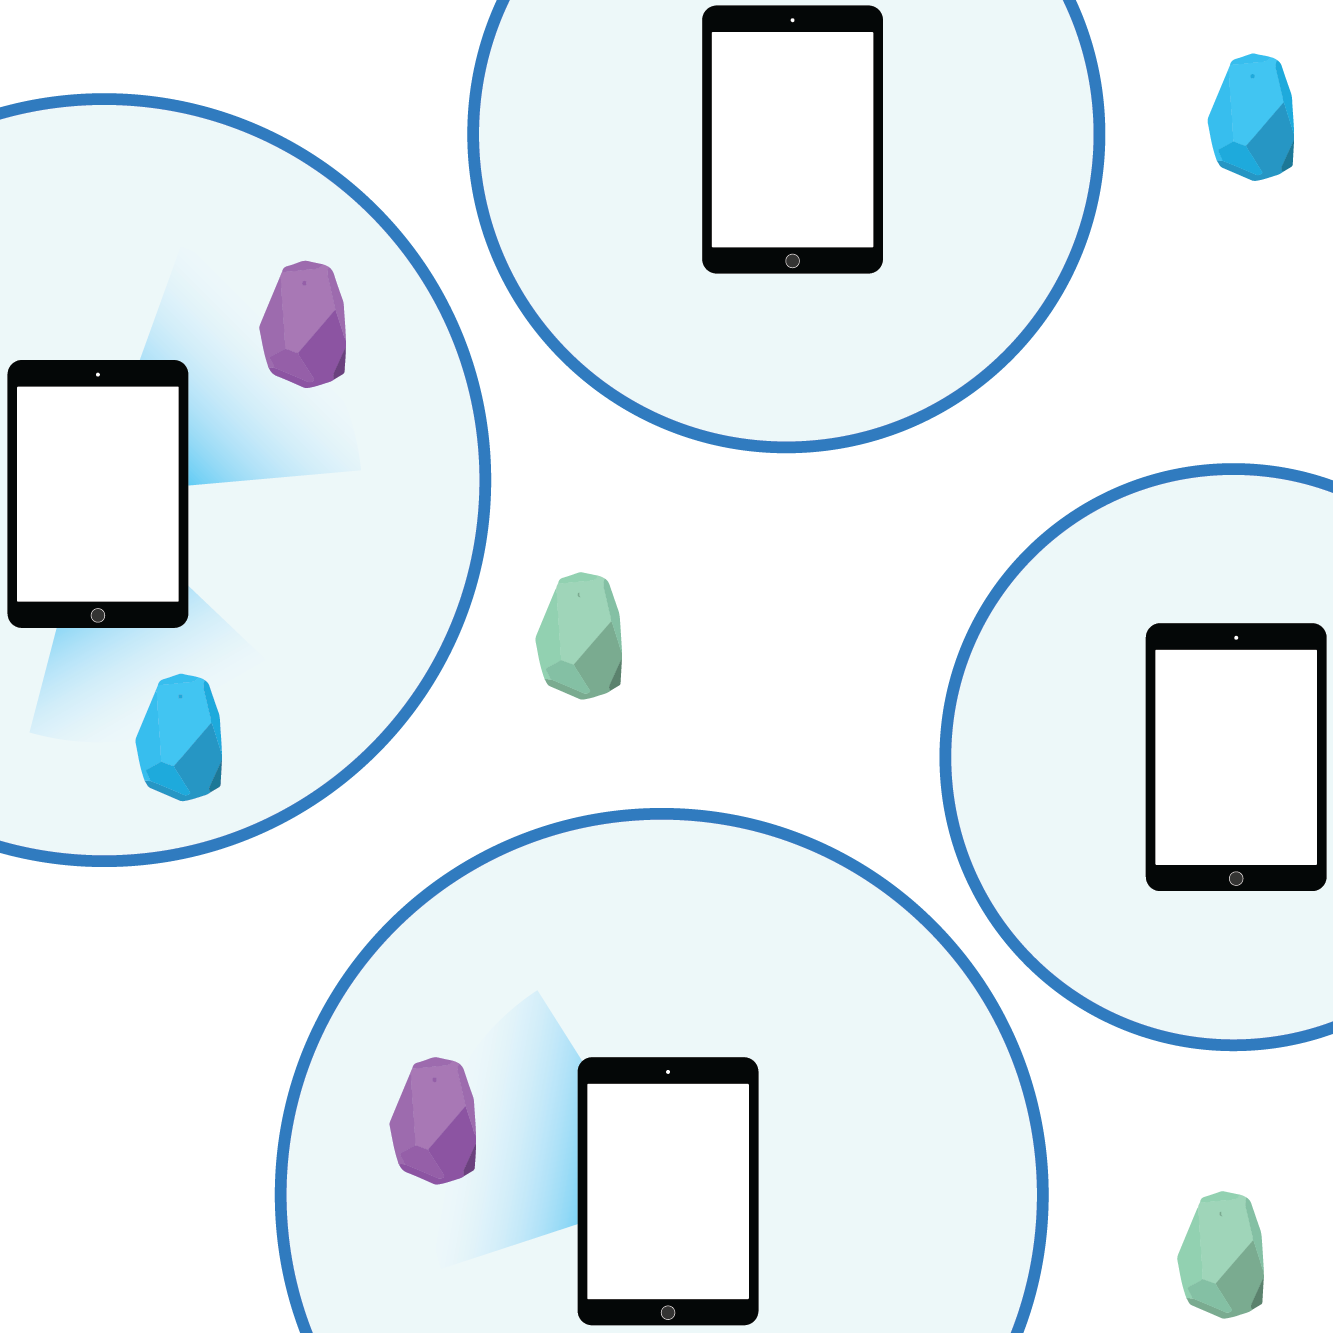
\includegraphics[width=2.5in]{images/room-places-use-case-1.png}
\caption{tablets tracking moving beacons}
\label{fig:use_case_1}
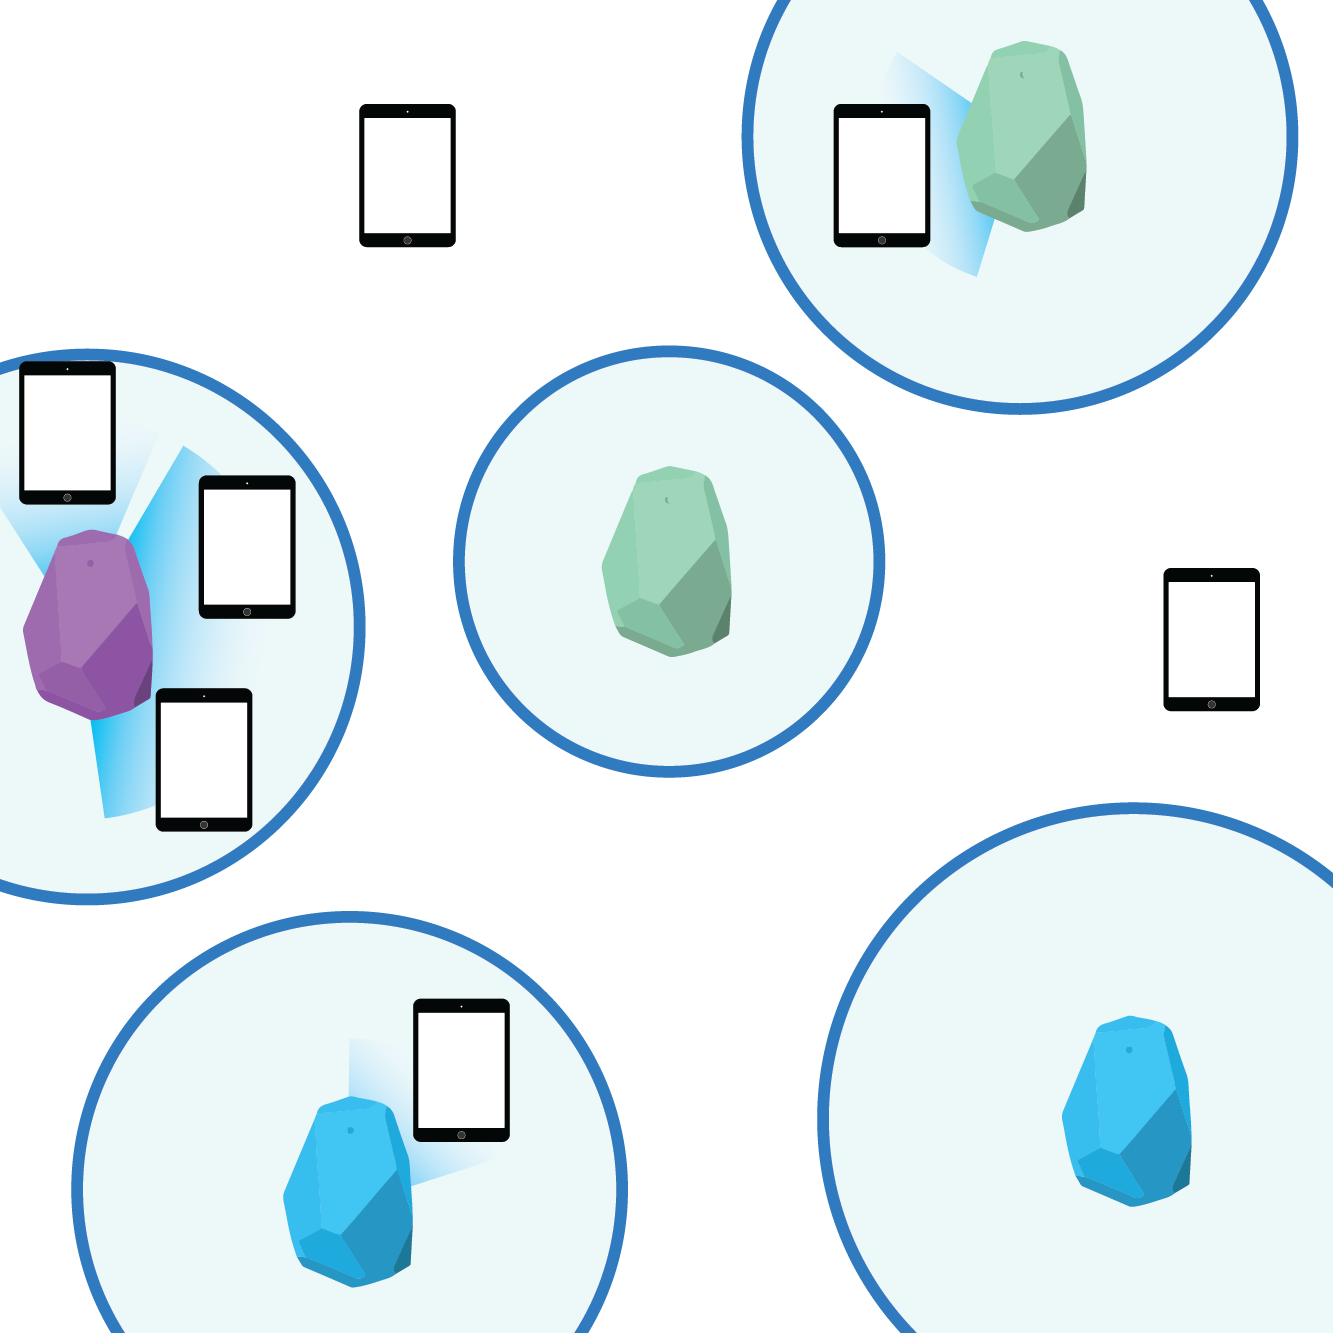
\includegraphics[width=2.5in]{images/room-places-use-case-2.png}
\caption{beacons tracking moving tablets}
\label{fig:use_case_2}
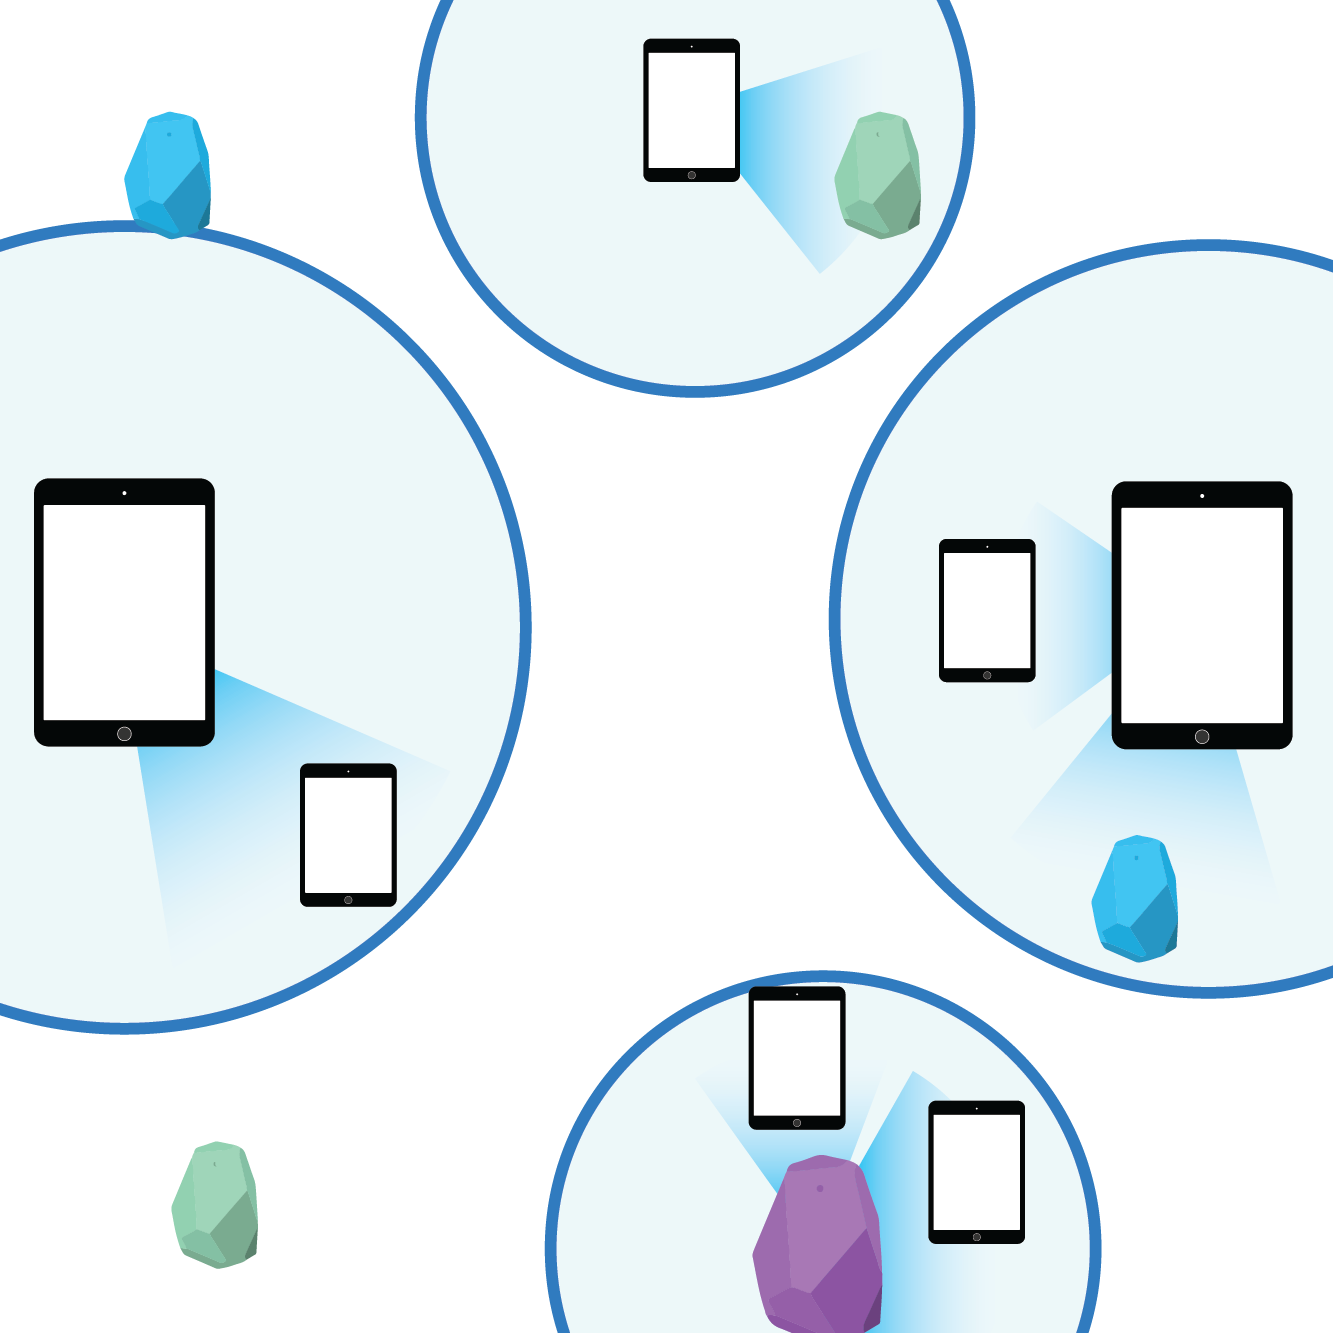
\includegraphics[width=2.5in]{images/room-places-use-case-3.png}
\caption{tablets and beacons tracking every Bluetooth LE device}
\label{fig:use_case_3}
\end{figure}

The first analyzed model and starting point for the discussion is the Apple iBeacon. It was created in order to deliver personalized content directly to the user smartphone when it is in proximity of a specific point. This technology is well suited for stores because it enables to target specific users with discount and promotions when they are near a specific product. In order to achieve this goal, a set of beacons is placed around the store, every one of them has a different code that transmits at fixed time interval on a certain radio frequency using Bluetooth LE protocol. Enabled mobile phones, when the store application is installed, are able to detect the beacon and they recognize it using its unique code and react providing personalized content to the user. An example on how, conceptually, this model was already applied inside learning sciences is Savannah project \cite{facer:savannah}, where mobiles were tracked (using GPS) used a fixed radio emitting infrastructure (the constellation of GPS satellites). 

The beacon model enables a new set of interactions that are based on the actual location of the user and it is ubiquitous for the characteristic of requiring very simple external hardware (iBeacons) and very low power that doesn't affect the duration of the battery of mobiles. Also the maintenance of beacons is very cheap since they can remain active for years with a small battery. This thesis proposes an improvement that can be obtained changing the assumption that the beacon must be the fixed object in the room and mobiles must change position. There are opportunities that are enabled using mobiles for tracking beacon positions. An important opportunity is the usage of location dependent collaboration resources: tangible objects containing beacons shared by many users that are associated with a possible interaction with the system. The interaction can depend from who is carrying the resource and from where the user (or an object) is in a precise moment.

In the following sub-sections, I report different systems that are already tracking radio beacons using a static positioned receiver and speculate about how much can be interesting adding flexibility to this models.

\subsection{Huting of the Snark}
In the Hunting of the Snark \cite{price:snark}, students investigate and discover characteristics of a virtual imaginary creature (called the Snark) hidden within the virtual space, co-located with the physical space of the classroom. Students use a number of physically-digitally coupled tools to locate and interact with the imaginary and elusive creature while it moves across "land, air and water" \cite{price:snark}. Technologies are employed in order to provide ways for interacting with the creature. An ultrasound based indoor tracking system is used in order to locate the PDAs used by children and provides an output dependent from their location. Another interaction happens using physical tokens that have to be placed at the entrance of a cave, and depending on the token used students can hear different "atmosphere" noises from inside the cave. In this context, two different ad-hoc systems were used, but there is the opportunity to unify them making easier to develop applications that use both.

\subsection{AquaRoom}
In AquaRoom \cite{novellis:acqua_room} students take the role of hydro geologists with the task of mapping a subterranean aquifer system (mapped to their classroom floor plan). Using this information they have to decide where to locate a new chemical plant within the local community to minimize potential environmental impacts. In order to accomplish this task, students "inject tracer dyes" and obtain water samples using a portable tablet-based "drilling unit". A suction cup attached to a (non-functional) cable is used to select locations for dye injection or water sampling. Test tubes capped with I-Buttons serve as simulated dye sources and sample repositories. Students "inject" dyes by inserting the test tubes into USB readers attached to the tablet drilling unit, with the liquids virtually running through the cabling. The interactive interface on the tablets allows them to manually mark the injection location, based on a grid system defined by the tiles on the room’s drop ceiling. Water samples are subsequently collected in a similar fashion, and tested for the presence of dyes using a simulated spectrometer represented by a shared desktop computer with its own USB reader. The injection of a dye followed by sampling allows students to establish the presence of an aquifer and the direction and rate of flow, which are marked on the tablet map and on a collective classroom map. This scenario highlights the need of a system that reliable recognizes under which tile the user is located without requiring a manual input. Since the position is discrete it could be easy to place fixed beacons near the tiles and associate the user position with the nearest beacon.

There is also another opportunity that emerges from this study: tracing the individual paths of the children while they're exploring the "subsoil" of their classroom. Since the position is self reported, can we trust it? Is it possible to combine user input with a tracking system prediction?

\section{Memory associated with physical objects}
The third contribution is describing and analyzing a technique for embedding information inside physical objects creating the concept of \textit{artifact as containers} or \textit{tangible containers}. The goal of the implementation explained in this thesis is not supporting every kind of data structure needed by applications, but is building a simple system complete enough for supporting the majority of the applications built in the past and creates the foundations for building more complex systems.

This contribution is driven by the need of creating a reusable system keeping track of virtual state of objects that can be combined with their location for creating new way of interacting with digital worlds. The opportunity to augment the reality with the information contained in tangibles: displaying personalized content on wall mounted screens or use every object as an authentication key for enabling hidden functionalities are only some of the new opportunities that are made possible with that capability.

Associating information with objects is not something new in Human Computer Interaction, actually it is done in every application development, but every time in a different and custom way depending from the features that are needed. Usually this is a task done in the back-end that has to be queried introducing latency and degrading user experience. I want to demonstrate that is possible to implement it in a distributed software scenario and is possible to introduce a hidden synchronization mechanism for separate the notion of data inside an object from the technology used for storing that data. In the next subsections I report different systems and I describe how they implement this capability in order to highlight the opportunity of simplifying the development process and include this capability in a framework.

\subsection{Hunger Games}
Hunger Games \cite{gnoli:hunger_games} is a participatory simulation designed to allow upper elementary school learners to explore fundamental concepts of competitive and cooperative games in the context of animal foraging. In Hunger Games the authors transform the physical space of the classroom into a natural habitat containing six food patches of different richness. Each student in the classroom receives a stuffed animal with an RFID tag embodied in it, which acts as his or her avatar during the activity. Whenever a student walks to a patch and places their avatar on top of it, the RFID reader embedded in the patch recognizes the tag and starts to provide energy to the student's avatar at a rate dependent on patch quality and competition (i.e. how many avatars are feeding off the same patch at the same time). After the activity students observe and reflect on their individual and collective foraging patters and design new strategies to improve their individual and/or collective outcome. In this scenario the tracking system made with RFID readers is completely separate with the system that store the energy levels of the avatars and that contains the parameters of the patches.

\subsection{BeeSim}
BeeSim \cite{peppler:beesim} is a participatory simulation which puts young children in the shoes of honeybees collecting nectar. The simulation makes extensive use of wearable technologies and aims at teaching kids about both the value of communicating nectar sources to other bees and the difficulty of finding nectar. Students assume the role of a honeybee looking for nectar by wearing a "ForagerBee" glove (a sensor embedded wearable made with LilyPad Arduino platform). Kids have only 45 seconds to collect as much nectar as possible (nectar level indicated with a led bar) while wrestling with the constraints of the system (e.g. limited nectar carrying capacity). Children take turns hunting for nectar. As the glove exchange happens, the child returning from the hunt can try to communicate the location of high-yield flowers to the “next bee”, through the use of nonverbal language. Once each child had their chance to wear the glove and hunt for nectar, the team with the most nectar is the “most prepared for winter” and therefore the winning team.

In order to collect nectar, the "ForagerBee” glove has a sensor that reads voltage over a resistor. Every flower (and the bee hive) has a different resistor that leads to a different voltage value reading. In order to store the amount of nectar collected, every glove is connected (using XBee wireless technology) to a central computer, that memorizes the amount of nectar collected and waits for the child to go to the bee hive for dropping it off. In this system, the proximity tracking  (made with a resistor and a voltage level sensor) and the nectar collected levels memory are kept separated introducing a series of challenges for the developers. They need a different resistor for every one of them making more difficult the initial setup because the voltage level must be measured for every flower. The substitution of broken resistors requires a physically identical resistor. 

\subsection{Virus Simulation}
Virus simulation by Colella \cite{colella:virus} is a \textit{participatory simulation} where students wore small portable computers called "Thinking Tags" around their necks with LED displays showing how many people every single individual had met during the activity and whether or not they are infected with the virus. The thinking tags are infrared receivers and transmitters that give the students the ability to transfer the virus to others by walking up to them. The goal of the activity was teaching to the students how to infer the rules that govern the simulation (e.g., virus latency, degree of contagiousness, who was the first infected agent, etc.). In this system the state of the objects is physically memorized inside the "Thinking Tags", since they are small computers, they have their own memory. This approach is successful in the scenarios where the information contained is changed only for the object itself and doesn't have to be accessed from remote objects (is not possible to know if an individual is infected or not until a teacher have physical access to the \textit{Thinking Tag}).

\section{High Level Application Programming Interface}
A very important feature, that allows all the three previously presented contributions to became a reality and the system to collaborate with external environments, is the presence of an high level set of APIs (Application Programming Interfaces). This feature is important in order to provide an easy and user friendly access to all the capabilities of the system. A technical description on how this APIs are implemented is present in the  \autoref{apdx:roomplaces_api}, in this section I explain what are the advantages and the motivations that drove the development of them.

The first motivation is related to the capability of the system of being ready to be used out of the shelf. During the development of scientific investigations for educational purposes the developer must spend the time implementing the application functionalities, not carrying about the technical details of the underlying technologies, in other words: I cannot expect a deep knowledge from the developer on how the system works. Reliable \textit{tracking system} and \textit{tangible containers} became a reality thanks to a huge amount of code (running on different machines) that manages the synchronization of all the components behind the scenes. Thanks to this APIs developers are allowed to use the tracking capabilities and tangible containers as services that can be used inside their environments and with their favorite programming language. The APIs are provided as simple native libraries (I implemented them in JavaScript, Swift and Ruby). 

An important point that I want to highlight and second motivation for using native APIs is that all the information is safely stored on a central server and the APIs are a simplified way for accessing and modifying this information. In case a component of the developed system crashes it is always possible to restore the state after the crash because all the objects provided by the APIs are synchronized behind the scenes. It is also important to safely store the data for research purposes: after the application stops when its time to analyze the data they can be found on the server, there's no need to use an external system for retrieving them from all the computers that run the application.

The third motivation for providing the needed information as a service is the possibility to integrate it in already existing systems. This is especially important for learning applications that are almost always developed iteratively and in which the functions are implemented in different moments. The user study in \autoref{chap:user_study} is an example in which the tracking system was used only in the last phase of the study and its integration did not require extra effort from the developer perspective. Integrating a tracking system inside pre-existing systems can enable new possibilities, for example is possible to create a distributed logging system that can track actions of the users (and safely store them on the central server) and report in real-time the behavior of the class to the teacher. Another opportunity is improving the security of the classrooms and compliance insurance: notify teachers or parents when children live the school if not previously authorized.

\chapter{RoomPlaces: tool for mobile and tangible interaction design}

\label{chap:room_places}

Room Places is an open source framework that supports the adoption of tangible interfaces inside classrooms. It is released as part of nutella framework \cite{nutella_framework}. This chapter describes its features, the internal software architecture, the configuration environments and provides a high level overview of the application development process using it.

\section{RoomPlaces architecture}
In this section I describe the software architecture of RoomPlaces and what are the assumptions and the implementation choices.

\subsection{The existing technology}
At its core, Room Places is powered by a robust framework called nutella. It was chosen because it embeds a set of technologies with the intent of supporting \textit{Macroworlds} \cite{gnoli:nutella} development and deployment in classrooms. The main technologies contained in nutella framework are: a robust message-oriented middleware (based on IBM's MQTT protocol) that connects all nutella components allowing to exchange messages and a document oriented NoSQL database called MongoDB that allows to store safely every kind of data in JSON format \cite{JSON}. It also provides simplified access to those technologies with a set of APIs that hide the complexity providing high level services like reliable channel oriented network and persistent data storages. A set of command line utilities manages the entire life cycle of a nutella application. Among the other commands there are utilities for creating and deploying applications inside multiple classrooms using only one server as backend, maintaining isolation between them. In order to be able to take advantage of all the functions of nutella framework, all parts of RoomPlaces are implemented as nutella components and for this reason every one of them contains \textit{nutella.lib} written in the native language of the component. They use the open-source nutella protocol for communicating with other components. The life cycle is managed by the framework, that abstract all the low level technical details like spawning one process for every class or connecting the components together. The goal of the nutella layer is to move designers and developers away from low-level communication primitives such as "connect", "re-connect", "disconnect", "keep-alive", "set timeout", "create process", "kill process" etc. and provide a set of more expressive communication APIs (e.g. "create a new class instance", "send a message to iPad1"). Nutella is divided in modules; every module takes care of one functionality. In \ref{fig:nutella_overview} is possible to see how the modules are wired together inside \textit{nutella library}.

\subsubsection{Nutella.net and nutella protocol}
This module implements the communication mechanism that allows every component to send messages over the network. It manages the persistent connection with the server, the automatic re-connection in case of disconnection and the reception and transmission of messages. All the network communications are based on MQTT protocol \cite{mqtt} that manages how messages are propagated on the network using a central broker installed on the server. Every nutella component that uses \textit{nutella.net} opens a persistent TCP connection with the MQTT broker and keeps it active for the whole duration of the application execution. When nutella is running inside a browser a websocket is used instead of a direct TCP connection: the browser opens a TCP connection automatically and runs websocket protocol over it. MQTT protocol is designed for dispatching messages using channel names: the sender component indicates the name of the recipient channel and the broker will deliver the message to every component that previously subscribed to that channel. The primitive offered by the libraries that implements the MQTT protocols are:
\begin{itemize}
    \item \textit{Subscribe(channel)}: indicates the intention to receive all the messages that will be sent to that channel. It is also possible to use wild cards for subscribing to more channels with only one request (e.g. "/channel/c1", "/channel/c2" and "/channel/c3" can be summarized with "/channel/\#").
    \item \textit{Publish(channel, message)}: send a message on the specified channel. The message can be a string, a number or a JSON \cite{JSON} object.
\end{itemize}
All \textit{nutella.net} messages are encapsulated inside MQTT messages, nutella protocol is used in order to provide a larger set of functionalities: 
\begin{itemize}
    \item \textit{Request}: Components can ask question directly to other components.
    \item \textit{Handle request}: Components can answer questions other components ask them.
    \item \textit{Publish}: Components can say things to an audience of components that are listening and are interested in what the "speakers" are talking about.
    \item \textit{Subscribe}: Components can express their interest in what other components are saying, listen and wait for them to say something.
\end{itemize}
These four actions can be grouped into two separate communication strategies: \textit{request/response} or pull (first two actions) and \textit{publish/subscribe} or push (last two actions). A base implementation of nutella protocol is provided by nutella library, available in multiple programming languages \cite{nutella_framework} and it is reported in \autoref{apdx:nutella_protocol}. The same channel can be used both with push and pull strategies. In \ref{fig:nutella_overview} is illustrated how components are connected together using a central MQTT broker (the MQTT broker used is Mosca \cite{Mosca})

\begin{figure}
\centering
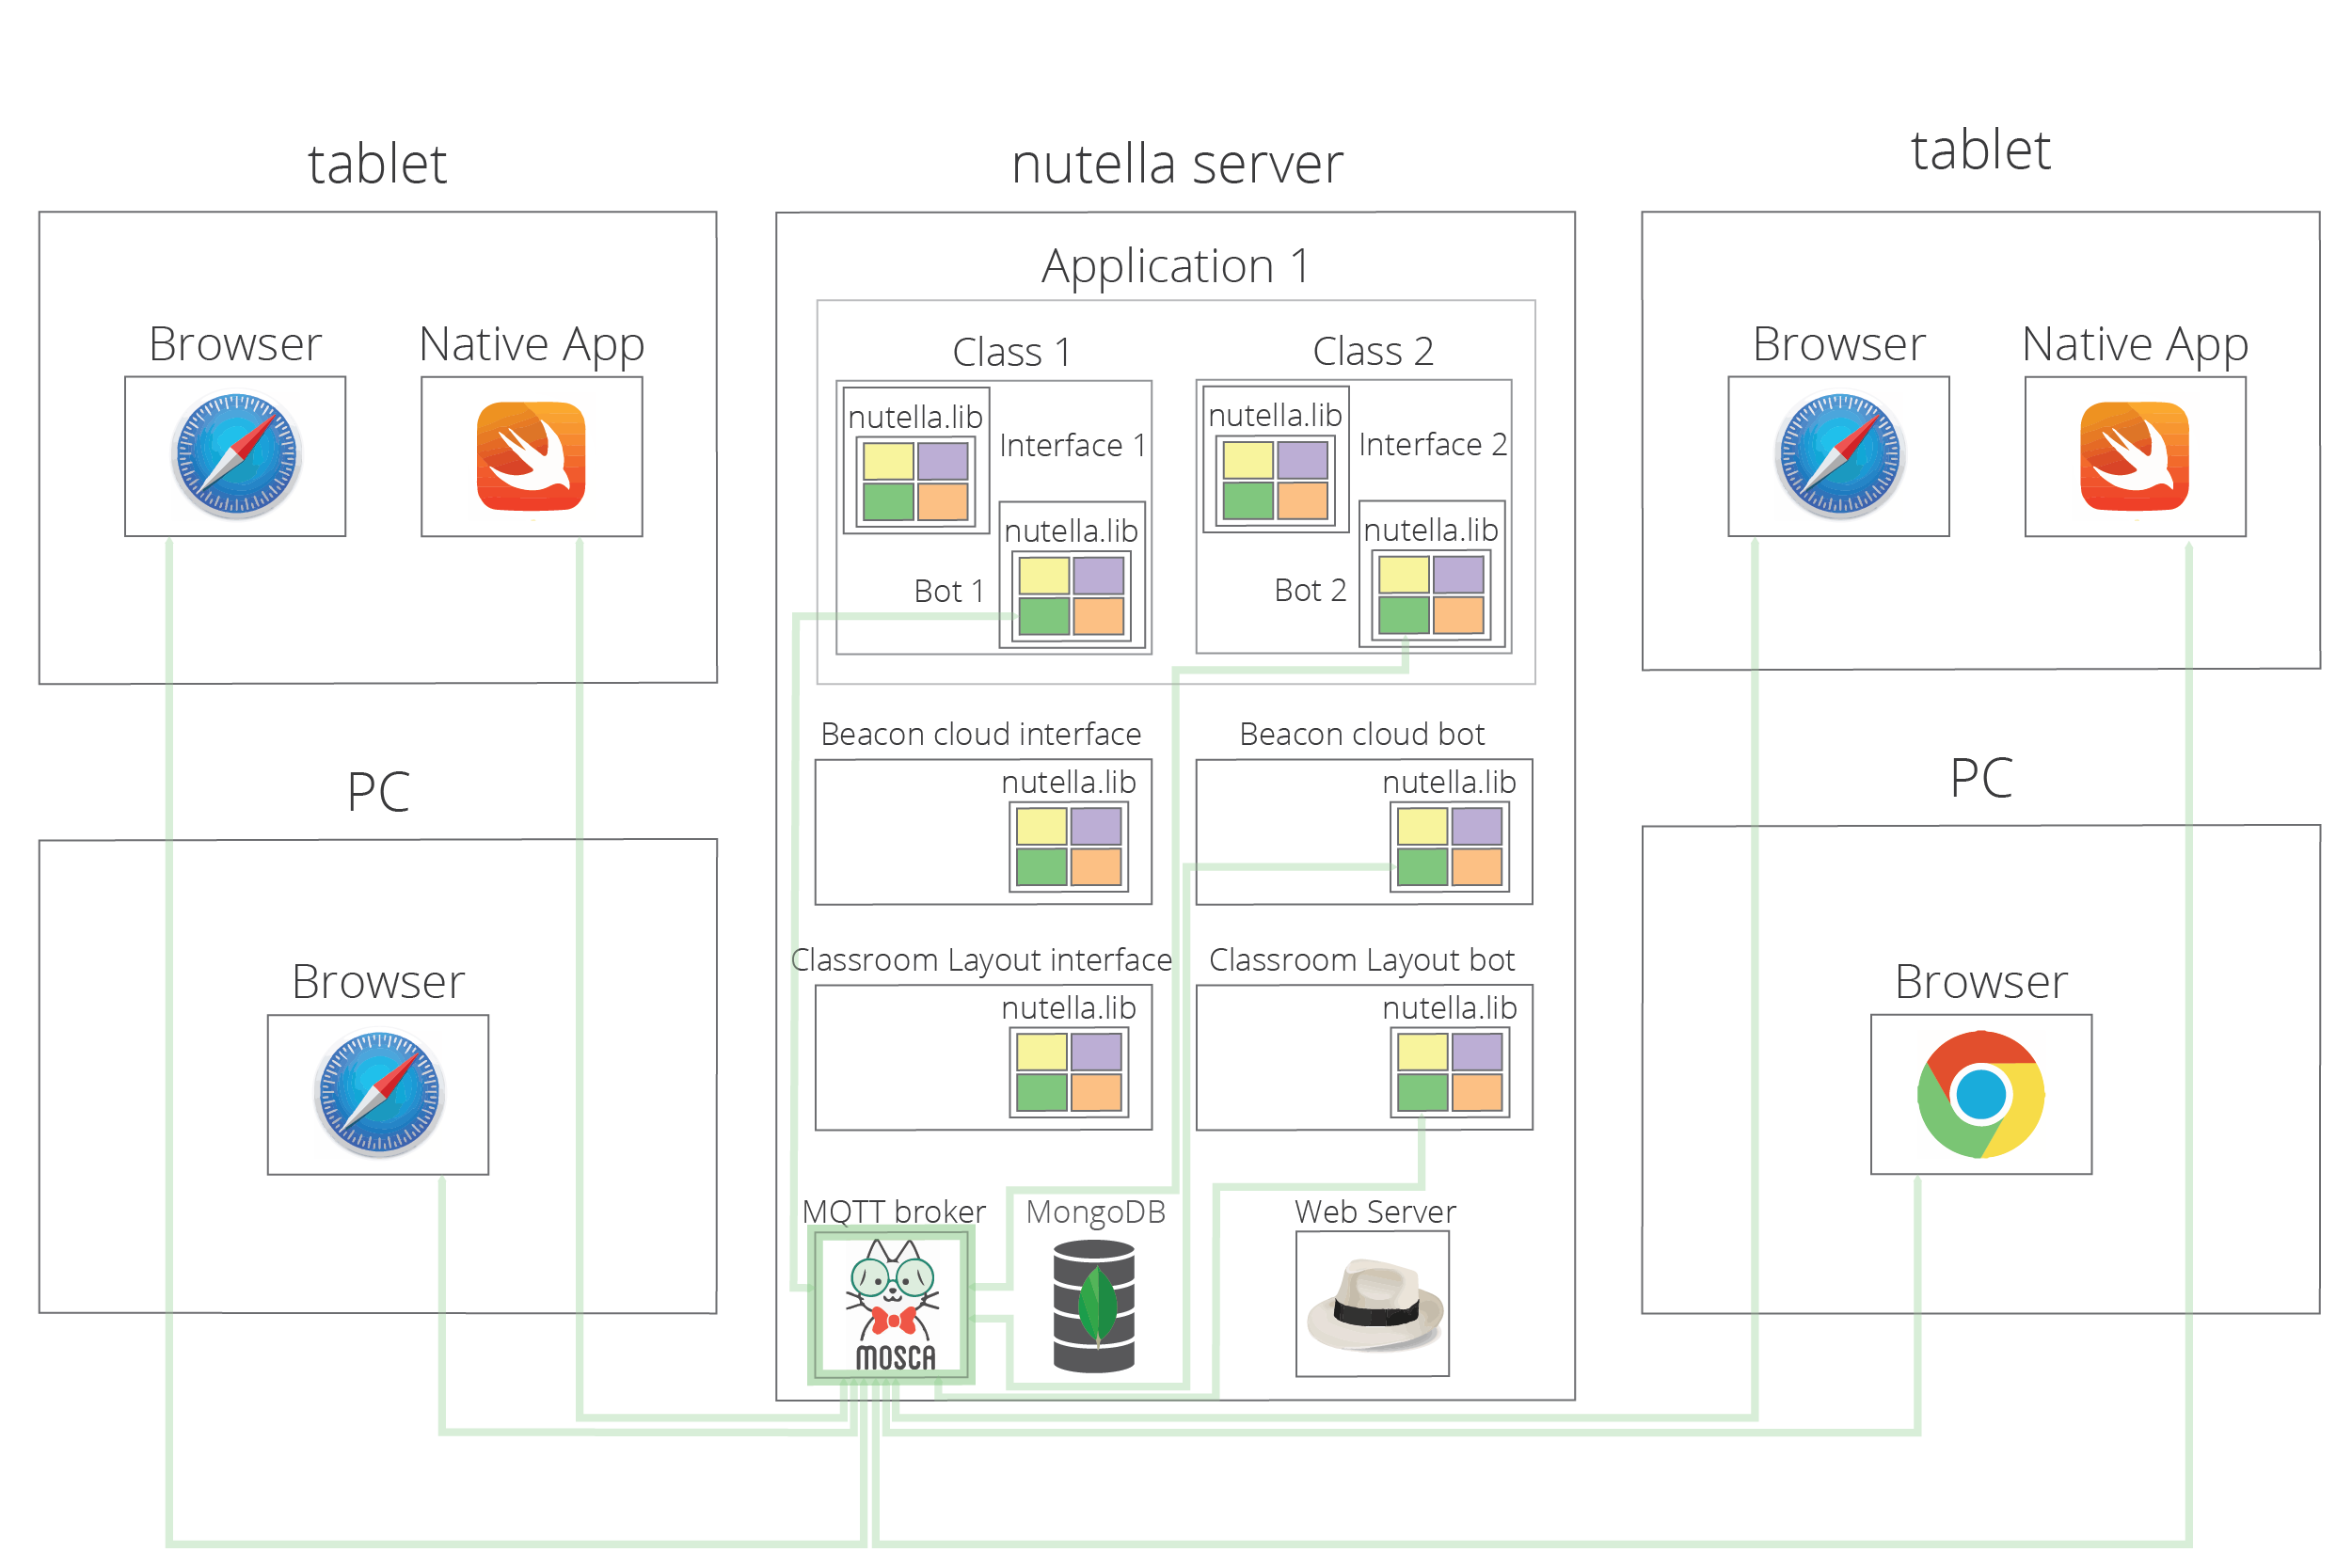
\includegraphics[width=6in]{images/nutella-client-server-broker.png}
\caption{connections between components realized using nutella.net and internal structure of nutella server}
\label{fig:nutella_overview}
\end{figure}

\subsubsection{Nutella.persist}
This module manages automatically the data storage on the central server using different technologies. It guarantees the isolation between different instances (called \textit{nutella runs}) of the same application and it makes data persistent also when a nutella component crashes. The technologies supported are:
\begin{itemize}
\item \textit{JSON file save}: save the information on a plaintext file using the json format.
\item \textit{MongoDB}: connects to a MongoDB server instance and store data in collections.
\end{itemize}
In order to create a persisted object, the developer has only to call one of the following primitives:
\begin{itemize}
    \item \textit{Json collection store}: creates an array stored in a plaintext file.
    \item \textit{Json object store}: creates an object stored in a plaintext file.
    \item \textit{Mongo collection store}: creates an array stored in a MongoDB collection.
    \item \textit{Mongo object store}: creates an object stored in a MongoDB collection.
\end{itemize}
The name of the object is a custom string that identifies the persisted object inside the current run.

\begin{figure}
\centering
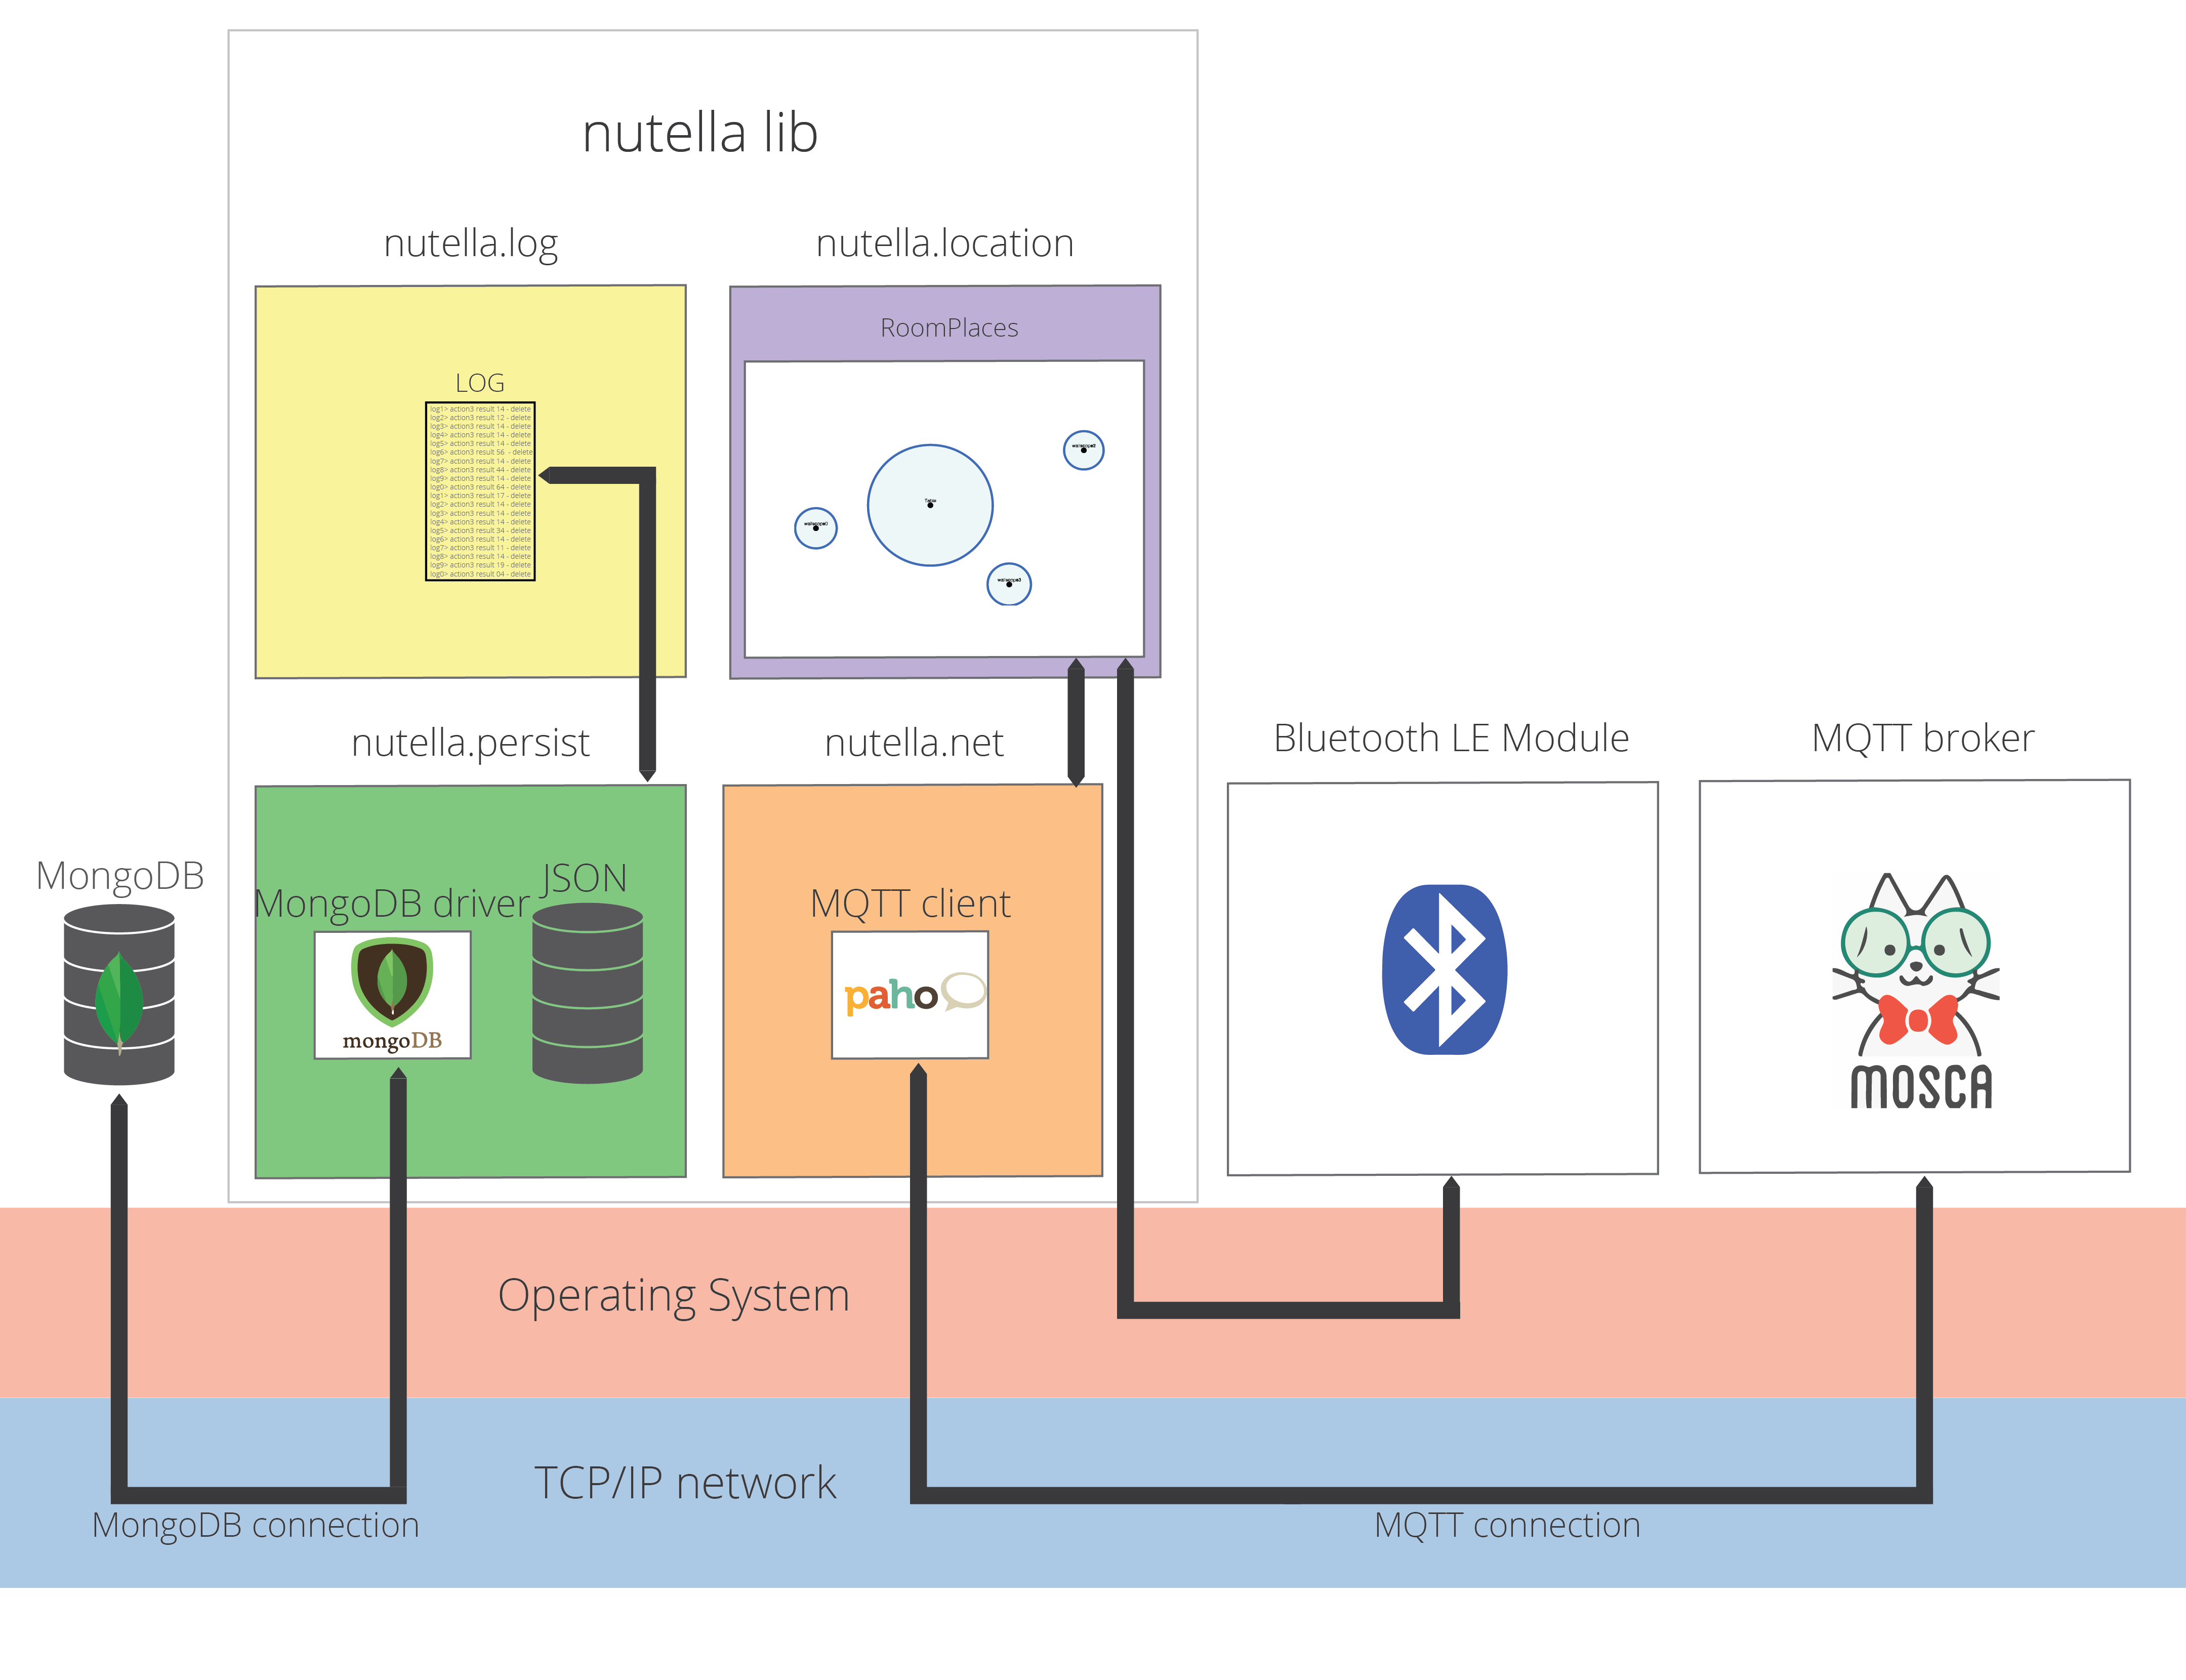
\includegraphics[width=6in]{images/nutella-overview.png}
\caption{nutella.lib components overview}
\label{fig:nutella_overview}
\end{figure}

\subsection{Tracking system}
The tracking system is based on Bluetooth LE (Low Energy) beacon technology. I chose a specific implementation of it called Apple iBeacon because it is a mature technology compared with the others that are present on the market, it is inexpensive and guarantees the compatibility with all mobile devices that use iOS operative system and are Bluetooth LE enabled (see \ref{tab:bluetooth_le_enabled} for all the available devices). It is also easy to scale and can track a theoretical unlimited number of users, and for this reason it is suitable for many tracking applications in hospitals \cite{yang:ibeacon}, museums \cite{he:proposal}, smart buildings \cite{corna:occupancy} and lastly the \textit{Classroom of Things}.

\begin{table}
\centering
\begin{tabular}{ | c | c | }
\hline
Device & Bluetooth LE enabled \\
\hline
\hline
iPad             & No \\
iPad 2           & No \\
iPad 3           & Yes \\
iPad Mini        & Yes \\
iPad Retina      & Yes \\
iPad Mini Retina & Yes \\
iPad Air         & Yes \\
iPad Mini 4      & Yes \\
iPad Air 2       & Yes \\
iPad Pro         & Yes \\
iPhone           & No  \\
iPhone 3G        & No  \\
iPhone 3GS       & No  \\
iPhone 4         & No  \\
iPhone 4S        & Yes \\
iPhone 5         & Yes \\
iPhone 5C        & Yes \\
iPhone 5S        & Yes \\
iPhone 6         & Yes \\
iPhone 6 Plus    & Yes \\
iPhone 6S        & Yes \\
iPhone 6S Plus   & Yes \\

\hline
\end{tabular}
\caption{Bluetooth LE enabled iOS devices}
\label{tab:bluetooth_le_enabled}
\end{table}

The iBeacon technology is mainly used for proximity tracking inside stores and its purpose is displaying promotions on customers’ mobile devices when the users approach a certain location in the store. 

The main hardware component of this technology is the beacon: a small device that consumes very low power and can remain active for years using a small battery. This device emits Bluetooth packets at fixed time frames, it contains an unique identifier and the calibrated RSSI (Received Signal Strength Indication) that is a parameter supplied from the constructor that allows the receiver to estimate the distance from the beacon.

Every Bluetooth Low Energy device can be a receiver component of the tracking system. The first prototype of RoomPlaces is built using iOS devices but every consideration is valid also for other mobile platforms like Android. iOS presents a native Swift API that allow RoomPlaces to query the Operative System for the nearby beacons: automatically the OS will receive all the beacon packets and will compare the calibrated RSSI field contained in the packet with the RSSI using a logarithmic model and a moving average filter for estimating the distance.

Room Places was built and tested using Estimote iBeacons \cite{estimote} with a packet emission frequency of 5Hz (one packet every 200ms) and transmission power of 4DBm, these parameters are a good trade-off between accuracy (directly proportional to the emission frequency and transmission power) and battery consumption for our application. An iBeacon configured in that way can work for six months with a single \textit{CR2477 battery} (1Ah at 3V for a total of 3Wh of energy) allowing every kind of application for one school semester.

\subsection{Integration with nutella}
RoomPlaces lives inside nutella framework, its back-end components run on the server as nutella bots and its interfaces are accessible using a browser through a web server called Sinatra (that is part of nutella framework and is illustrated in \ref{fig:nutella_web_server}). This is an high level description of how the framework works. When the developer creates a new application nutella will generate empty bots and interfaces directories. Bots are back-end programs that run on the central server and interfaces are web pages that are transmitted to the client and run inside the client browser. The development  process of an application consists is inserting code inside bots and interfaces in order to generate the desired behavior of the application. For lunching multiple instances of the created application is necessary to use the command \textit{nutella start run\_id}, where the run\_id is the name of the new instance of the application (for example the name of the class in which the application will run). Every instance of bot can be used in only one class, there's not theoretical limit on the number of instances that can be created. The framework will ensure the isolation between classes and guarantees that every change on the state of one class will not be reflected in the other classes. It is important to highlight that in nutella architecture the code is shared between all the instances, but the state is saved on plaintext files or inside a MongoDB collection in a separated directory and for this reason it is possible to update the code and modifying the data independently. It is also possible to update the code and replace run-time some bot instance without suspending the exectution of the others.

\begin{figure}
\centering
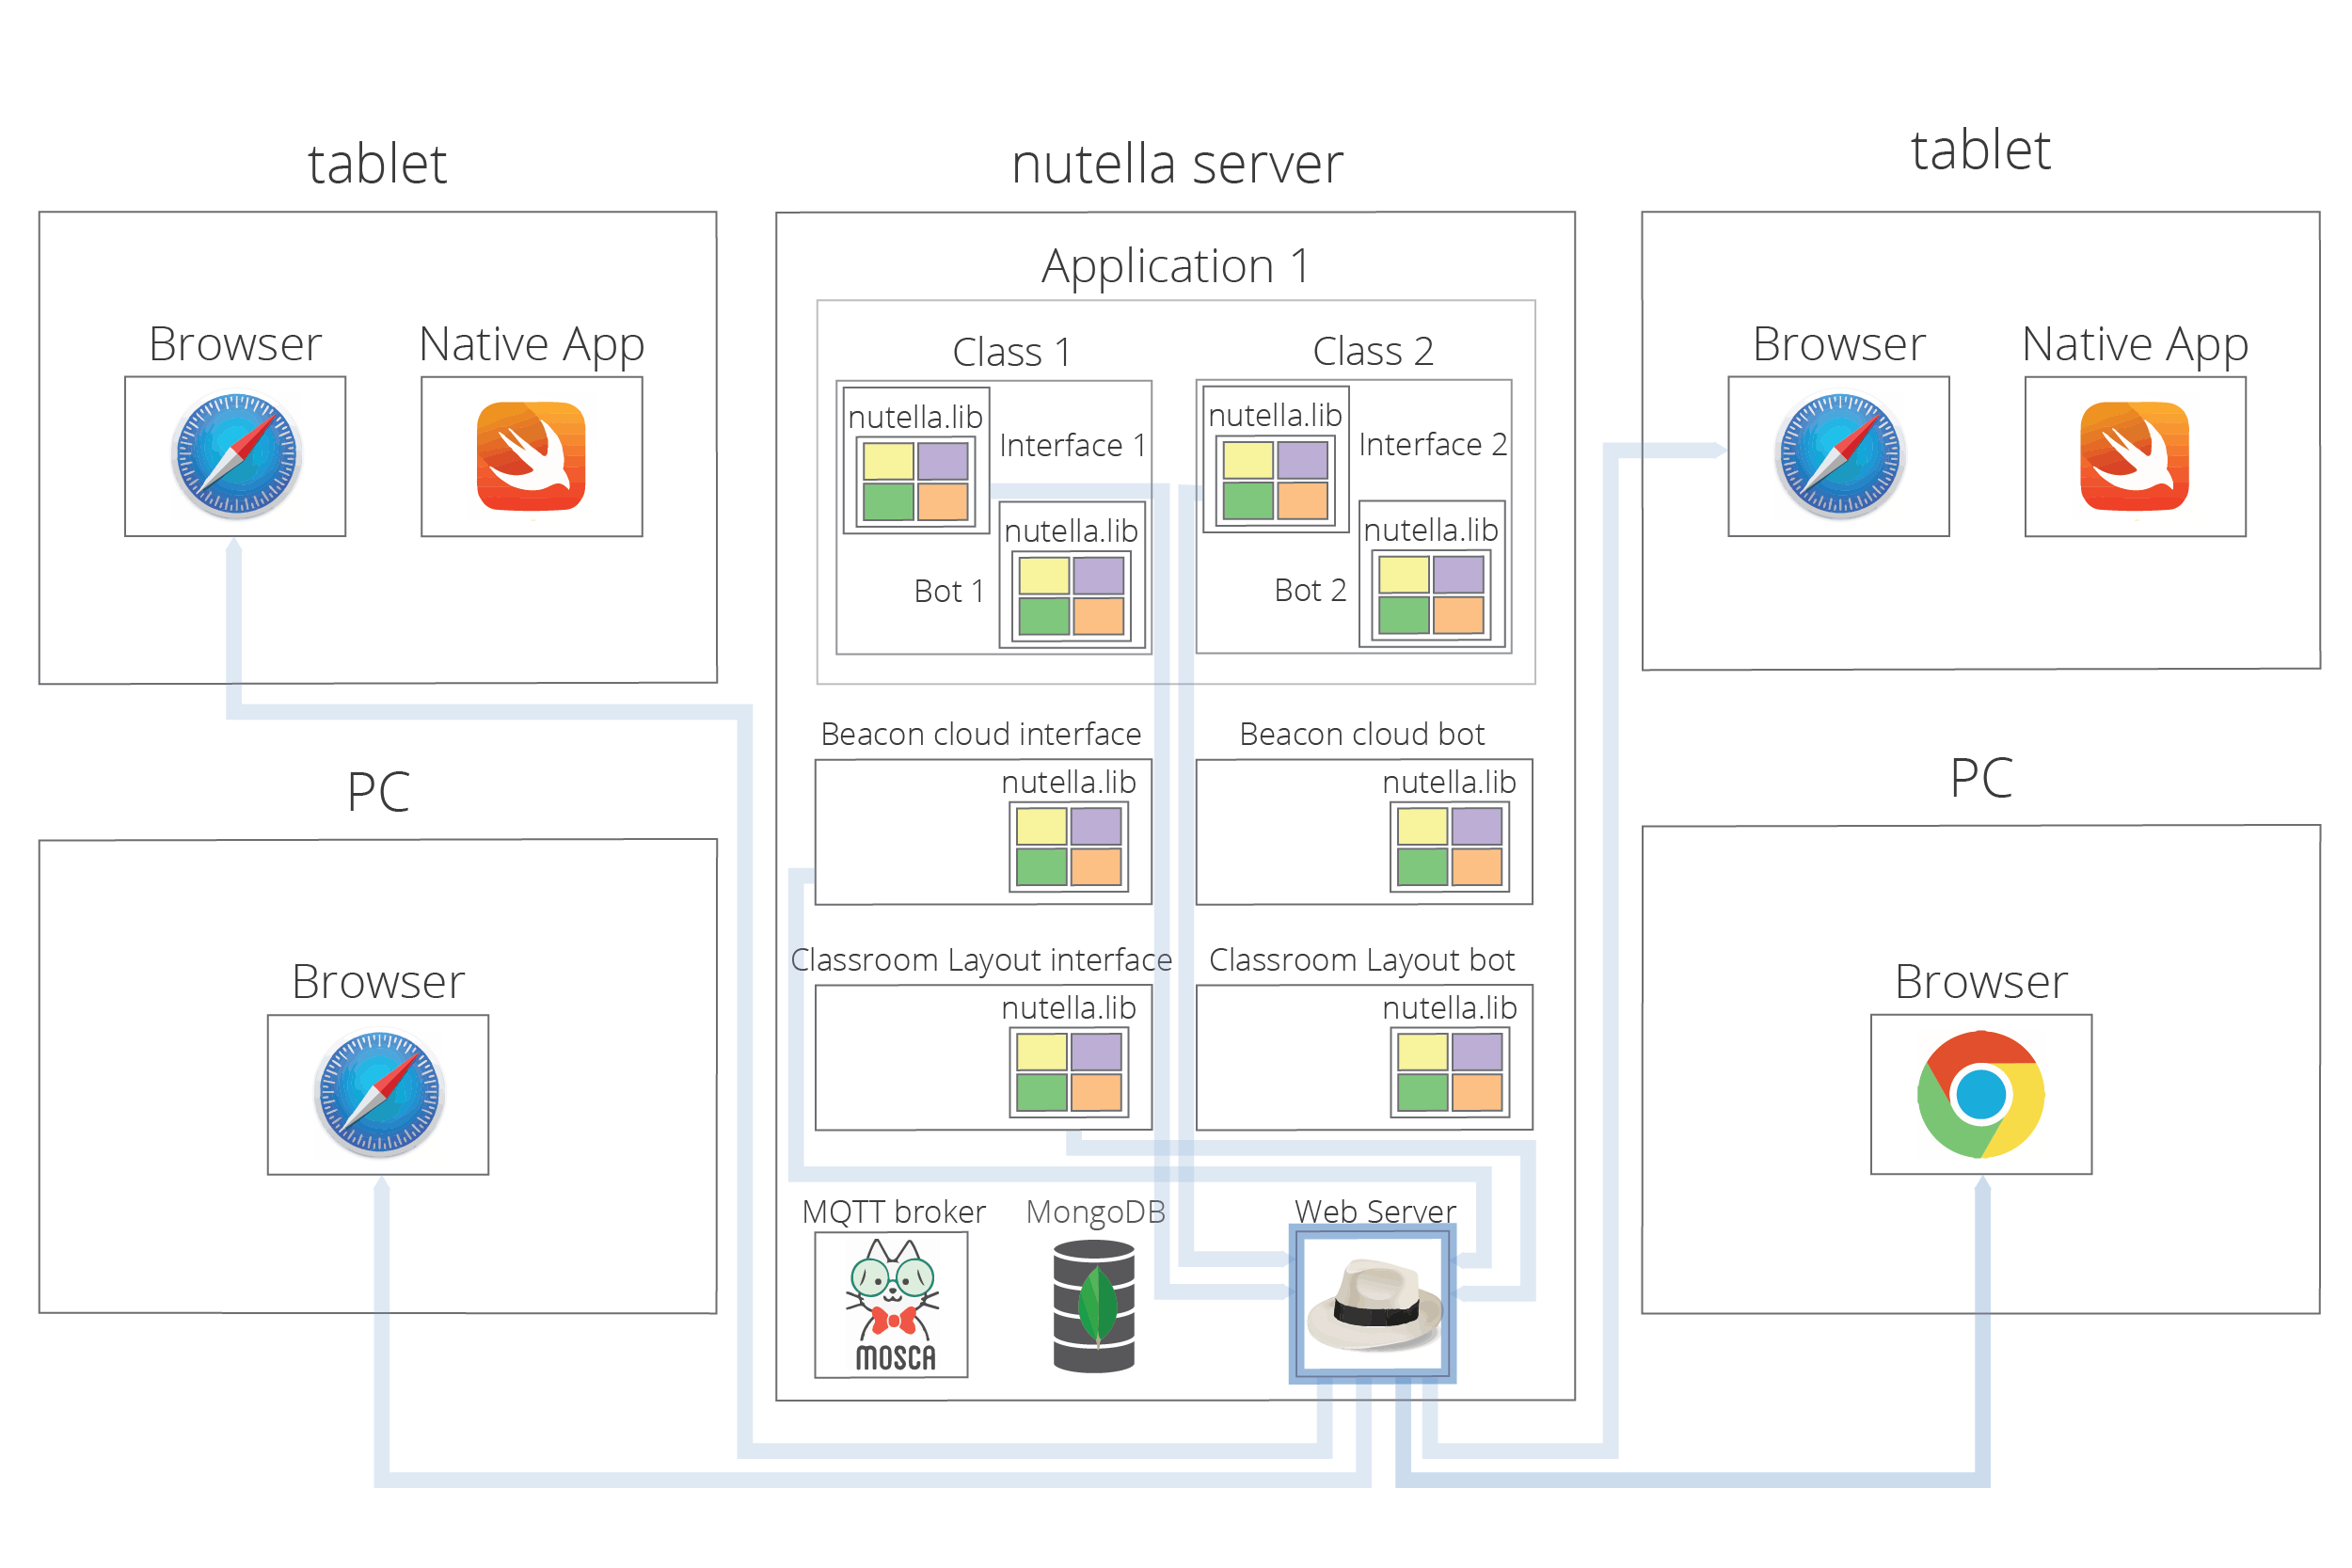
\includegraphics[width=6in]{images/nutella-client-server-webserver.png}
\caption{nutella interfaces distributed though Sinatra web server integrated in \textit{nutella framework}}
\label{fig:nutella_web_server}
\end{figure}

\subsection{RoomPlaces definitions}

RoomPlaces main purpose is tracking \textit{resources}. A \textit{resource} is an entity in the 2D classroom space, it can be a \textit{beacon} or a \textit{mobile device} (tablet or phone) and it is identified by an unique \textit{RID} (Resource Identifier, an alphanumeric string) assigned by the developer. There are two types of resource: \textit{static resource} has a fixed position and it is used as a reference point for tracking other resources, \textit{dynamic resource} can move: its movement can be manipulated using the APIs (contained in nutella.location) or automatically tracked. Static resources have a proximity radius that is the maximum distance in which they can sense other objects, everything farther than that is ignored.

There are two types of coordinate systems supported by Room Places: continuous and discrete. They can coexist in the same room and every static resource belongs to one of them. The axis on the discrete coordinate system can be both configured for expressing the coordinates with integer numbers or letters.

Dynamic resources can be manually positioned using one of the two coordinates systems (through RoomPlaces APIs) or can be automatically tracked using the proximity tracking system. In the latter case the position is automatically assigned if the resource is close enough to a static resource. For determining the proximity, the estimated distance between the dynamic and the static resource is compared with the static resource radius.

\subsection{Core components}
The most important component of Room Places is called \textit{RoomPlaces Bot} and at every time there's one instance running that serves multiple classes at the same time. Nutella framework bots are special back-end components that are instantiated only once during the nutella startup procedure and are always running in background. This component translates a stream containing distances between static and dynamic resources (generated by mobile devices) into an high level representation of the classroom resources. There are two functionalities provided to other components: a query system and a push notification service. The first one allows a component to request the position of a resource at any time (pull functionality) and the second allows a component to subscribe to a specific event (related to the proximity of resources) and be notified every time that the event occurs (push functionality). All the components are illustrated in \ref{fig:nutella_web_server}.

\subsubsection{Classroom Layout}
\textit{Classroom Layout} is a nutella interface used in order to configure RoomPlaces Bot. It is a static web page that communicates with the Bot and it allows the user to create resources, configure the role (static or dynamic) and the coordinate system that is desired (continuous, discrete or automatic proximity tracking). This interface is designed for being used by developers but also in the future by teachers that will include the tangibles that are present in their classroom.

\subsubsection{Beacon Cloud}
\textit{Beacon Cloud} is a nutella interface used for adding beacons to the set available in Classroom Layout. This interface (shown in \ref{fig:wallcology_beacon_cloud}) associates three numbers that are needed for identifying an iBeacon (UUID, major, minor) with the RID that is assigned to it. The numbers are inserted only once when the beacons are purchased. The beacon information is stored into a component called \textit{Beacon Cloud Bot} that has the capability to be queried for the list of all beacons present in the system (needed by the iPads that need to identify if nearby beacons belongs to the system or not).

\subsubsection{RoomPlaces Location Tracking}
\textit{RoomPlaces Location Tracking} is part of the standard nutella library (module \textit{nutella.location}) and is available on mobile platforms. It is implemented in Swift for running on iOS operative system is packaged as an iOS framework that can be easily included in any application. An instance of it runs on every iPads and iPhones. It contains the routines that query the operative system for the beacons physically around the device and compare the beacon identifiers (UUID, major and minor) with the values contained in Beacon Cloud Bot list in order to understand if a relevant beacon is found. The output of this component is a list of beacons with the relative distance from the device where the software is running. It communicates this list to Room Places Bot every second: iOS APIs update the list with 1Hz frequency and for this reason the delay of the tracking system cannot be lower than 500ms in average, 1000ms in the worst case. When the device is configured as a dynamic resource (the software must query Room Places bot for discovering this information), Room Places Location, will request Beacon Cloud for obtaining a virtual beacon identity and will start broadcasting beacon packets. Every time that Beacon Cloud creates a virtual beacon it informs all the components that a new beacon is present in the system and from that moment on they can start tracking it. This process is completely transparent to the developer.

\subsection{RoomPlaces communication protocol}
For allowing RoomPlaces components to communicate it is necessary the sets of rules described in the the open-source RoomPlaces protocol. It is a message oriented protocol based on nutella protocol: every message is encapsulated inside a nutella message and sent over the network taking advantage of the nutella connection (it uses MQTT protocol and eventually websockets when running inside browsers). This choice enables to use the set of network abstractions provided by nutella: the \textit{push/pull} communication methods over channels, the isolation between different instances of the same application (running in different classrooms), the automatic server address discovery and connection management (for automatic reconnection). The protocol is described in details in \autoref{apdx:roomplaces_protocol}.

\subsection{Application Programming Interfaces}
On top of this existing layer of technology sits an abstraction layer provided by RoomPlaces, what I call the APIs layer \cite{nutella_location}. Its goal is providing an easy access to RoomPlaces functionalities enabling the developer to interact with all its components without knowing RoomPlaces protocol. The APIs are consistent over all the platforms and implemented inside \textit{nutella.location} module.

There are two main functions inside the APIs: the first is retrieving resource objects and read/write configuration parameters on them as they were local objects, this is a \textit{pull} functionality because it allows the developer to know the state of one resource at any time. The synchronization mechanism (with the other RoomPlaces components) is voluntarily hidden, there's no need to explicitly tell when to send or load data on the server. The second functionality is subscribing to specific events; this is a \textit{push} capability because it notifies the application when the event occurs without the need to constantly query the server looking for changes. The supported events are generated by dynamic resources that enter or exit the range of a static resource. This is the effective mechanism that implements the \textit{event stream} and allows a lightweight interaction with tangibles when the goal is sensing the proximity between objects.

In order to implement the \textit{tangible containers} (storing information inside physical objects) every resource object retrievable using the API has a set of key value pair. Adding or modifying a key value pair will automatically insert the data inside the object and propagate the modifications to the whole system.

This set of APIs is designed keeping in mind the iterative nature of the macroworld development process: there's a feature that I call \textit{continuous resource update} that allow the resource object list present in the API to continuously listen for resource updates. The consequence of this feature is the possibility of adding, removing and modifying resources without the need of restarting all the other components or polling on the server. Another effect is that every resource object inside the list is constantly up to date (when position or other parameters change) reducing the query delay (compared with the standard client-server implementations where a remote component must be called every time a get request is executed). The \textit{continuous resource update} is implemented with a push mechanism: every client is waiting for updates subscribing to a nutella channel (using the \textit{subscribe} primitive provided by \textit{nutella.net}), when an object is modified an alteration message is sent and is instantly propagated through the network. In order to increase reliability all the alteration messages are checked by \textit{RoomPlaces Classroom Layout} component and not propagated to other components in case the contain errors. A detailed explanation of the RoomPlaces APIs can be found in \autoref{apdx:roomplaces_api}.

\subsection{RoomMonitor}
It is another part of nutella framework and it is developed in order to enable the developer to inspect components of the system, discover problems and to send alert messages in case of crashes. The first goal is achieved using the interface visible in \ref{fig:nutella_monitor} that displays the components in a circular interface where the dimension of the components are proportional to the number of channels that are used by that component. The connection between components are realized with white lines. It is also possible to show all the messages sent on every connection clicking on the links. The second function of this component is enable the system administrator to insert an e-mail to be notified every time a system component crashes. This function is useful while the system is running inside classrooms because provide instant feedback when something goes wrong. The application instances that run into classes can be inspected singularly using the selection menu on the left of the interface. The number of problems are also reported (in the orange circle) in order to quickly see the state of every classroom instance.

\begin{figure}
\centering
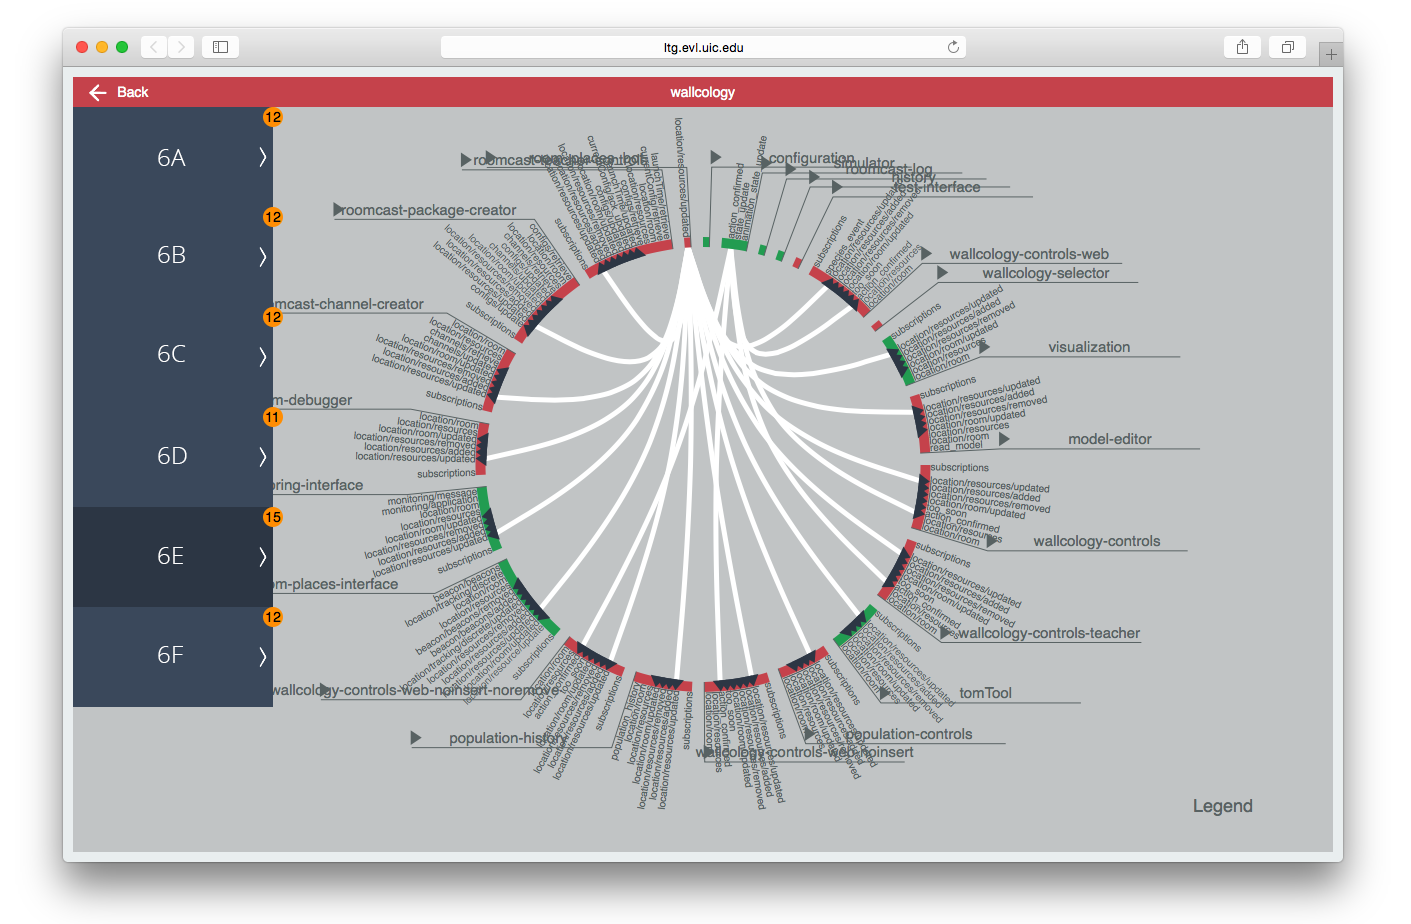
\includegraphics[width=6in]{images/nutella-monitor.png}
\caption{nutella RoomMonitor interface. On the left there's the menu for selecting the classroom instance, on the right the components disposed in circle and wired using nutella channels represented with white lines.}
\label{fig:nutella_monitor}
\end{figure}

\section{Configuration environments}
Inside RoomPlaces there are two configuration environments that allow the software developer to describe the physical room and assign name and roles to objects. In this section I describe their characteristics. The names are used for retrieving information about the object using the APIs. The first environment is Beacon Cloud, it is a list of beacons that will be used inside classrooms, the interface is unique for all the classrooms since the technical characteristics of the beacons remain the same (UUID, Major, Minor). The second interface is called Classroom Layout and is different for every class. It shows the objects that are tracked inside the classrooms and allow to chose name and roles. Both of them are accessible on the nutella landing page (that is personalized based on the class).

\subsection{Beacon Cloud}
It is a web interface created with the purpose of being the only point in the system that deals with the technical details of beacons. It has a table that contains all the physical beacons that are used in classrooms and for every one of them the RID and three numbers that uniquely identify it: UUID (Universally Unique Identifier), Major and Minor. For inserting a new beacon there's an empty line at the bottom, basic integrity checks are executed in order to ensure that the input is valid. There's also the possibility of changing parameters for a beacon already present in the list. All the changes are propagated real-time to all the other components of the system: this feature allows the developer to continuously add, remove and modify beacons during the development phase.

\subsection{Classroom Layout}
It is the main configuration interface for RoomPlaces. The purpose of it is allowing the user to insert all the physical resources that must be tracked inside the virtual space. It is composed by two graphical components: on the left there's a map of the classroom that shows the resources already present with their names. It is also possible to change the room dimensions modifying the quotations.

\begin{figure}
\centering
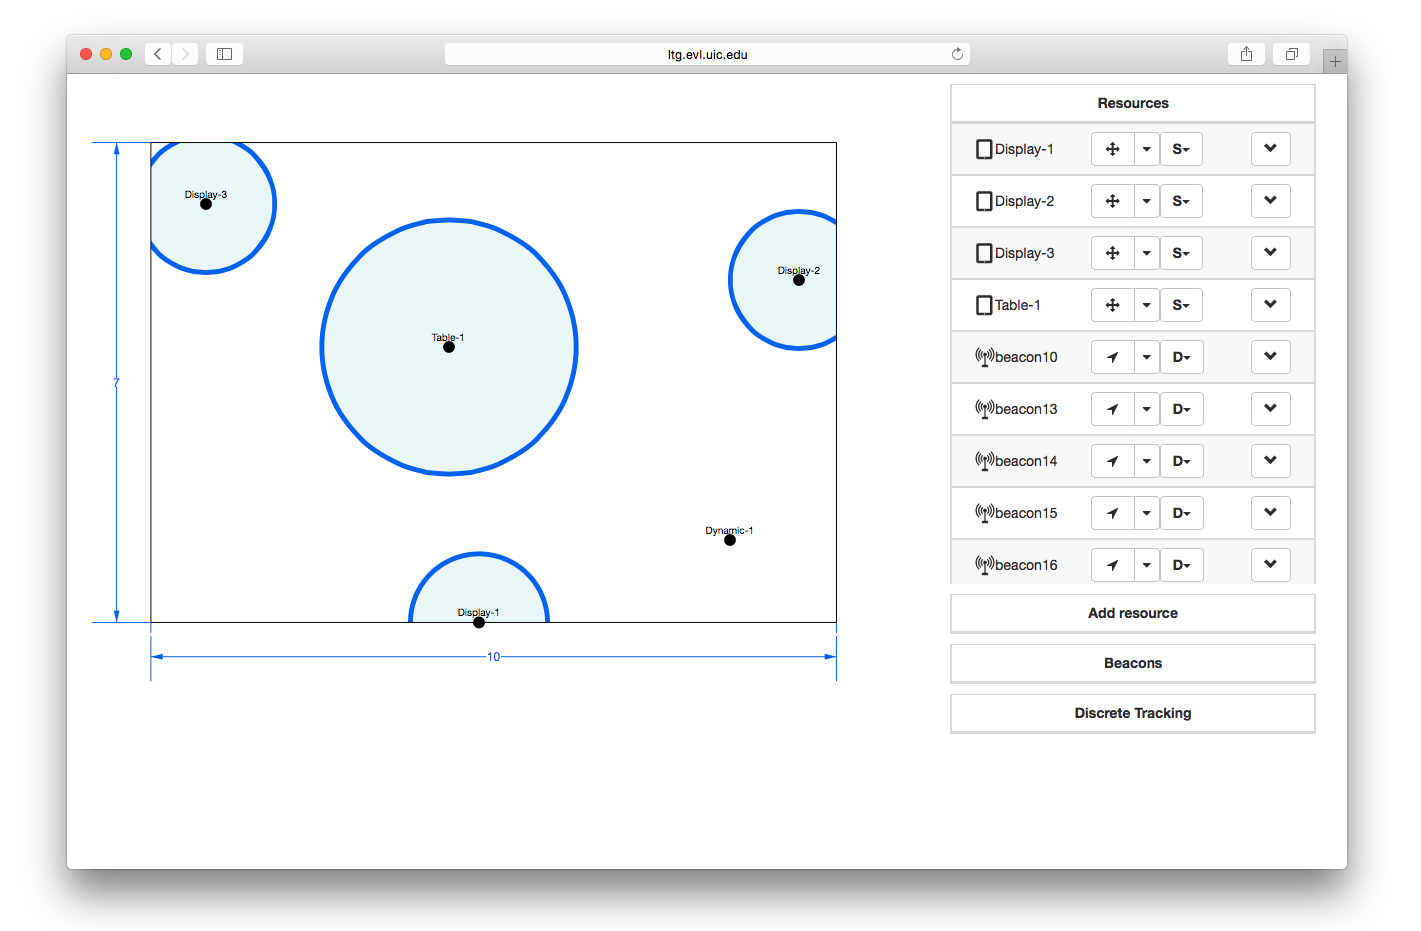
\includegraphics[width=6in]{images/classroom-layout-map.png}
\caption{Classroom Layout interface with the typical scenario configuration}
\label{fig:classroom_layout_map}
\end{figure}

On the right side there's a menu with add, remove and edit functionalities. It is divided in four sections as shown in \ref{fig:classroom_layout_map}. The first section list all the resources that are already tracked in the class, for every resource is possible to configure the coordinate system (continuous or discrete) and the role of the resource (static or dynamic). Every resource has also a contracted menu that can be expanded that contains a number of additional parameters: position in the 2D space according to the chosen coordinate system, proximity radius for static resources and a set of key-value pairs that allows to insert information associated with that resource.

\begin{figure}
\centering
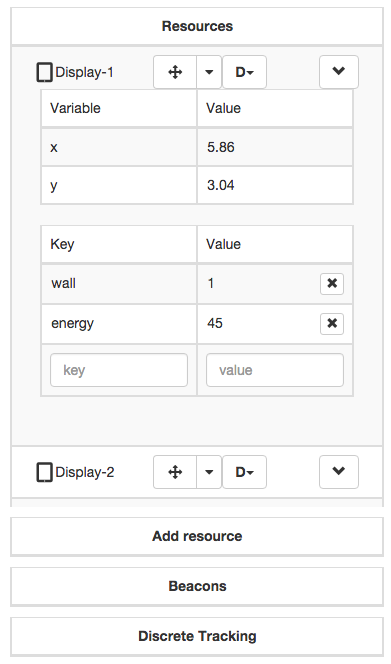
\includegraphics[width=1.9in]{images/classroom-layout-resources.png}
\caption{Resources menu that allows to modify the parameters of the resources in the system}
\label{fig:classroom_layout_resources}
\end{figure}

The second (\ref{fig:classroom_layout_add}) section is used for adding a new resource: it allows to chose the type of device, the coordinate system used and the role. 

\begin{figure}
\centering
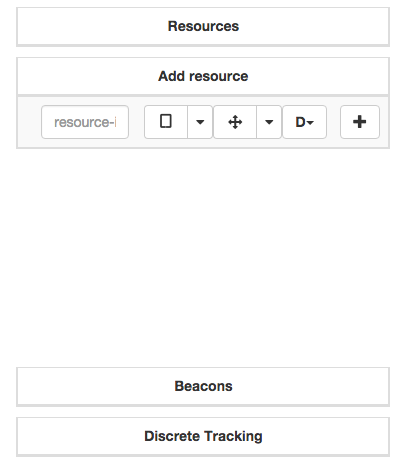
\includegraphics[width=1.9in]{images/classroom-layout-add-resource.png}
\caption{Add resource menu that allow to insert new resources to the system}
\label{fig:classroom_layout_add}
\end{figure}

The third (\ref{fig:classroom_layout_beacons}) allows to pick a beacon from the list provided by Beacon Cloud, clicking on the add button the beacon will automatically be configured as dynamic resource automatically tracked in continuous coordinate system.

\begin{figure}
\centering
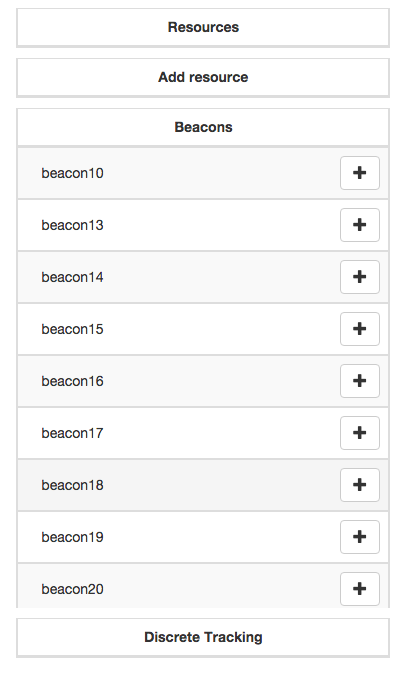
\includegraphics[width=1.9in]{images/classroom-layout-beacons.png}
\caption{Beacons menu that allows to insert beacons resources that are already in Beacon Cloud list}
\label{fig:classroom_layout_beacons}
\end{figure}

The last section in the menu (\ref{fig:classroom_layout_discrete}) is dedicated to the configuration of the discrete tracking system. Since this system coexists in the same room at the same time with the continuous one, it is possible to map one over the other. The user can control every aspect of this mapping inserting continuous coordinates and dimensions of the discrete tracking system external rectangle and the number of cells. The other configuration parameter is the possibility of expressing discrete coordinates with letters or numbers because a possible use case is that the user will insert the coordinates in the system and using letters for one axes and numbers for the other one minimize the possible errors.

\begin{figure}
\centering
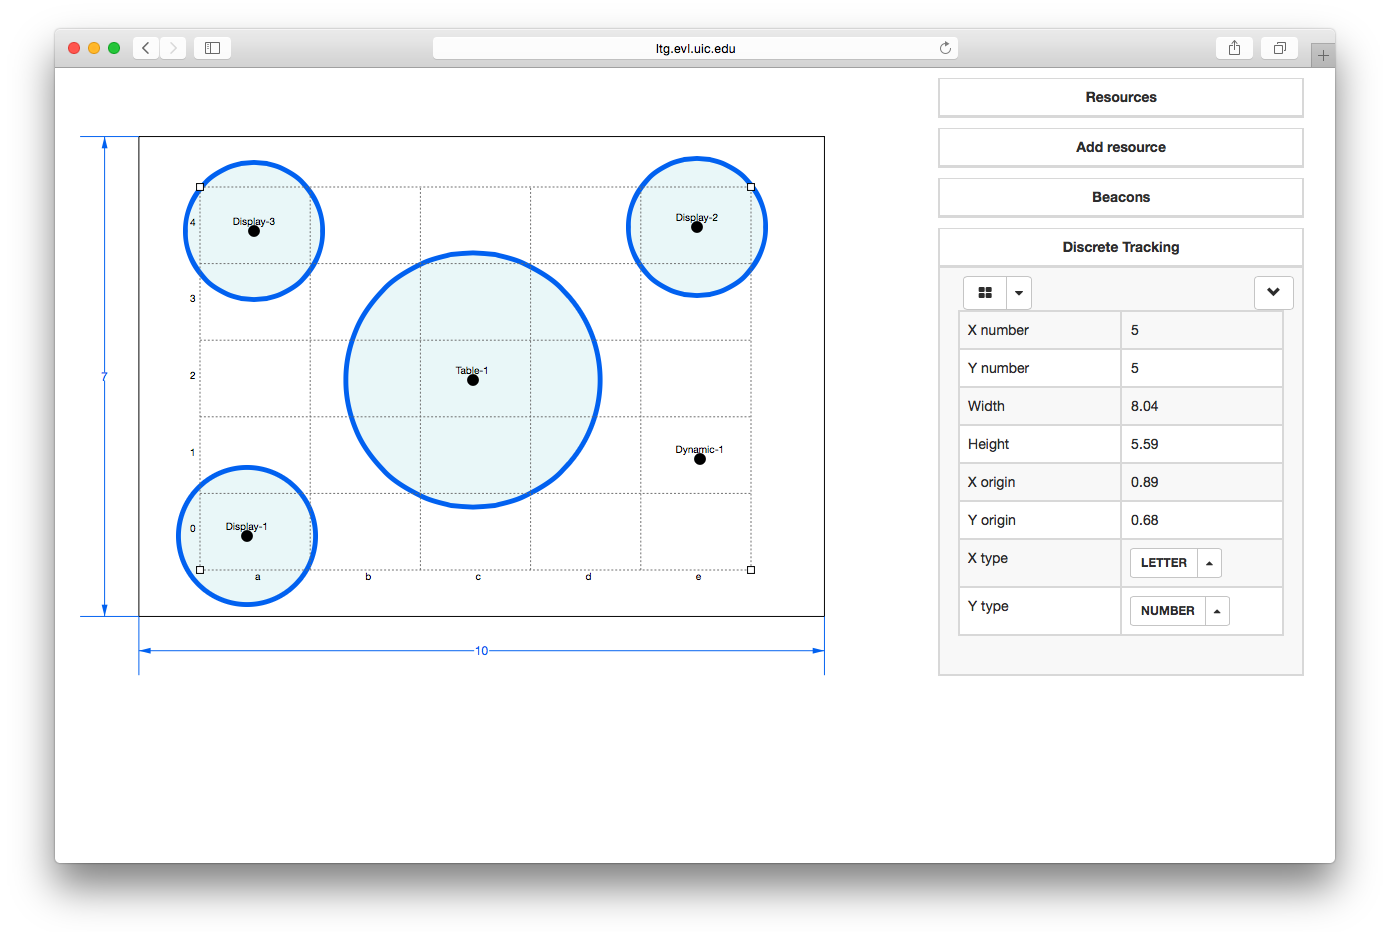
\includegraphics[width=4.5in]{images/classroom-layout-discrete.png}
\caption{Discrete coordinate system represented on the map. When the coordinate system is modified also the resources that use it are moved accordingly on the map.}
\label{fig:classroom_layout_discrete}
\end{figure}

The map always displays in real time the state of the classroom. It is possible to drag and drop all the static resources for changing position. Every one of them has a proximity radius represented with a blue circle. All the dynamic resources with a distance lower than the radius are considered in proximity of it. Dragging the radius on the map will modify that parameter according to the graphical representation. On the map is represented the discrete coordinate system and the resources that use it, on the edges there are signifiers (little squares) that can be moved for modifying the shape of the external rectangle. The map is useful also for debugging purposes: every time a dynamic resource is considered in proximity of a static resource it is displayed using a circle with a radius equal to the estimated distance. 

\section{Tangible interface development with Room Places}
The framework components described above, together with nutella framework, were designed for supporting the entire development process of new applications (macroworlds) that take advantage of tangible interfaces for interacting with the simulation. I will go through every phase of the design and I show how the different parts of RoomPlaces support the developer in those phases. In the next chapter, I will go into more detail and provide specific examples of how RoomPlaces addresses the challenges described in \autoref{chap:lit_rev}.

\begin{figure}
\centering
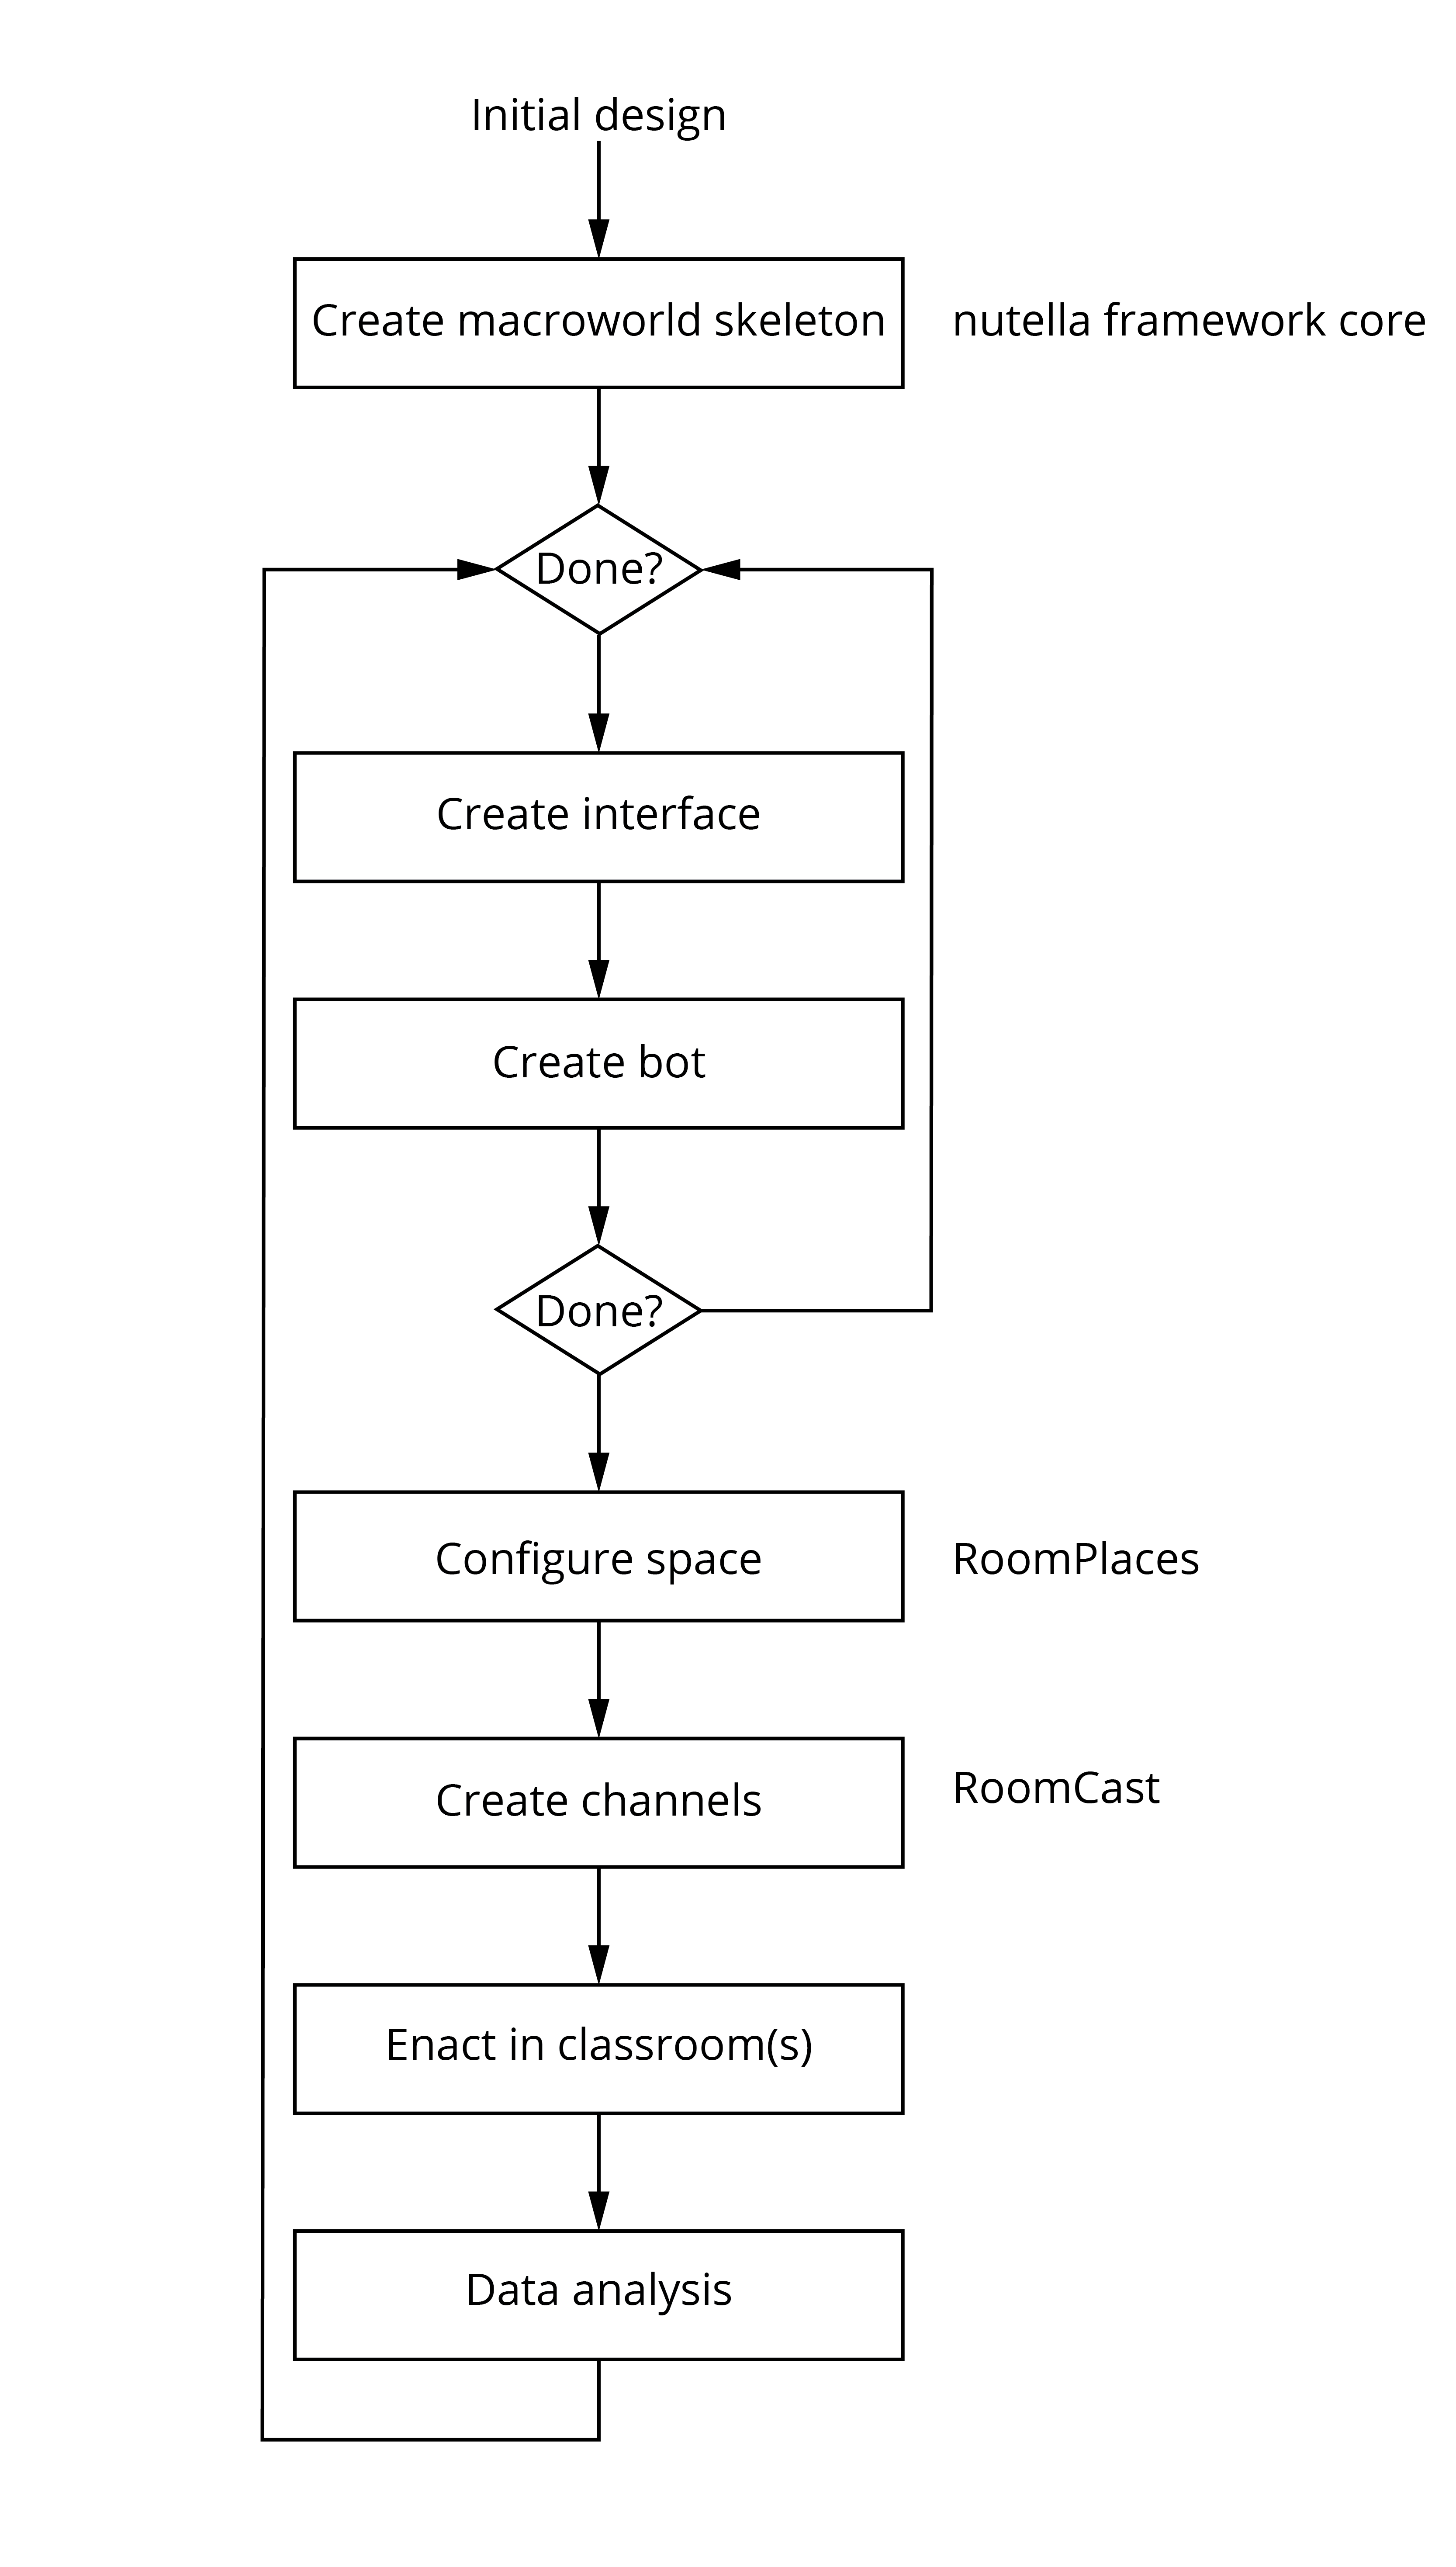
\includegraphics[width=3in]{images/nutella_workflow.png}
\caption{Macroworld design and implementation general workflow with nutella and RoomPlaces}
\label{fig:nutella_workflow}
\end{figure}

\subsection{Initial design and beacon purchasing}
The first step in designing a macroworld application is to decide what to build. It is important to point out that the design and development processes are tightly coupled and highly iterative. RoomPlaces \textit{continuous resource update} capability was designed for supporting this process allowing the developer to start and stop components as well as adding, removing and modifying resources without worrying about the synchronization with the server (that is totally transparent when using the APIs).

RoomPlaces is one of the components needed to design a macroworld, for this reason it is useful to contextualize it inside the nutella application design. In the \ref{fig:nutella_workflow} there's an overview of the entire development process using nutella. It is useful to observe the \textit{space configuration} step that involves RoomPlaces is repeated many times until the desired result is obtained and the application meets all the goals of the developer, for this reason several iterations must be supported and no hypothesis can be done on the order of the actions that must be executed on the configuration interfaces.

After the initial design is known, the designer must decide what are the interactions that can be supported with a tangible interface. No assumptions were made in RoomPlaces on the number of resources and the dimension of the tracked space, the limit is the creativity of the macroworld designer. After the initial tangible interaction has been designed it is necessary to build or buy beacons. The beacons can be shared among classrooms, minimizing the number of beacons that are needed. The suggestion in this phase is to always buy more beacons than needed, this is for replacing eventual broken beacons, this replacement is supported by RoomPlaces and can be done on the fly, thanks to \textit{continuous resource update}, without restarting any component.

\subsection{Environment configuration process}
When the beacons specifications (the three numbers that identify every one of them) are known it is necessary to insert them in \textit{RoomPlaces} using the \textit{Beacon Cloud} interface. All beacons are inserted in this cloud regardless their constructor and from this point on they will be referenced using the name inserted in \textit{Beacon Cloud}. From this interface is possible to add or remove beacons in successive iterations.

For configuring what objects have to be tracked there is the \textit{Classroom Layout} interface that allows the developer to insert beacons from a list (the \textit{Beacon Cloud} list). From this interface is also possible to insert resources with an arbitrary name into the room and assign a position to them. It also useful for debugging: every time that a dynamic resource is detected it is automatically displayed on the map. This feature allows the developer to start testing the configuration before writing the first line of code. It is also useful during the development phase of every cycle because it is possible to see arrival and departure events without the need of writing an external logger for them. As the previous interface also Classroom Layout will remain available all the time for future modifications during the development and those modifications can be done on the fly for supporting incremental application development of more components of the system.

\subsection{Code development process}
This is the process that takes the specifications and translate them into components of the macroworld. Every programming language is supported in this phase because all the protocols used are open-source, although the nutella library is already provided in JavaScript, Ruby and Swift languages because past experiences in macroworld development suggested them as most popular languages.

There are two methods for interact with RoomPlaces: using the APIs provided in nutella library and make requests and subscriptions directly to \textit{RoomPlaces} bot using \textit{nutella.net} or directly an MQTT client library. The fist is simpler and requires the programmer to call only functions already implemented taking advantage of the layer of abstraction that APIs provide. The latter is useful in the scenarios where a component has to be implemented in a language in which nutella library is not provided. If the developer choose this option it is necessary to understand  RoomPlaces protocol and how the components are wired together using nutella network library (\textit{nutella.net}).

If the developer decide to use the APIs all the needed tools are provided inside functions and data structures of \textit{nutella.location}. The most important data structure for bootstrap the components is \textit{nutella.location.resources}: it is an array of resources that can be used in every moment for accessing objects properties in the room like tracked location and stored parameters. It is also possible listen to arrival and departure events. For all the technical details see \autoref{apdx:roomplaces_api}.

After some iteration, when the code is developed and tested is time to deploy the application inside the classrooms. For doing it is necessary to use the command \textit{nutella start runid} on the server that creates a new instance of the application. When a new application instance is created a new instance of every bot is created and wired with the other components. During the time in which the application is running RoomPlaces \textit{Classroom Layout} interface can be used for looking how resources are moving in the class and for detecting eventual anomalies. In order to monitor the general behavior of the application, how components are wired together and if some component crashed it is possible to use \textit{RoomMonitor} interface entirely developed for this purpose and visible in \ref{fig:nutella_monitor}.

\chapter{Exploratory Study: two months at the primary school}

\label{chap:user_study}

In this chapter I report an \textit{exploratory study} about the usage of tangibles conducted in primary school on upper elementary students. The goals of this study are: collecting evidence that RoomPlaces is able to support a real use case inside a classroom and explore how it is possible to take advantage of tangible user interfaces in order to create new type of learning activities. The research questions of this exploratory study are:

\begin{itemize}
\item How do teachers and learners coordinate their use of shared tangibles?
\item Can the use of tangibles motivates the students? Can the need for coordination of shared tangibles creates opportunities for productive disciplinary engagement? (Engle and Conant \cite{engle:guiding}) Do they become cultural artifacts (a la Horn \cite{horn:role})?
\end{itemize}

The research questions are intentionally grouped in two sets: the first one is about the mechanisms that students use for access to the tangibles, the second is about the effective benefits that tangibles give to the learning experience.

In order to develop the software application used for this study, \textit{RoomPlaces} was used in combination with \textit{nutella} framework for building an interactive ecosystem simulation called WallCology that is a well known \textit{Embedded Phenomena} invented by Moher \cite{moher:wallcology}. The application was written from scratch using the capabilities of nutella and RoomPlaces for rapidly developing the final prototype.

In the next sections I explain the context in which the study is conducted, how WallCology was built with an emphasis on how RoomPlaces was used to support the study, the method that I used for collecting and analyzing data and the results obtained in this study.

\section{Context description}
WallCology study was run in parallel in three classes, of 16 primary school students each, for two months. Every class worked on its own state of the simulation: as other \textit{Embedded Phenomena}, \textit{WallCology} has a state in every time instant, also when the students cannot observe it. This state is represented by the number of creatures present in a certain ecosystem. There was no contact at all between classes, the same activities were done in all the classes in order to compare the outcomes.

\subsection{WallCology}
The version of WallCology implemented for this user study is an improvement of the original prototype presented in 2008 because the technology used for developing it is more advanced and knowledge from the previous study was used in order to improve the user experience. WallCology is a virtual ecosystem \textit{simulated investigation} that runs continuously from the first day until the last that is used. The uniqueness of this \textit{Embedded Phenomena} is in the used metaphor: eleven different species of creatures live inside the walls of the classroom, they populate the entire wall and small parts of them are made visible using virtual tools called \textit{Wallscopes} made with a PC running a computer graphic simulation shown in \ref{fig:ecosystem_1}. 

\begin{figure}
\centering
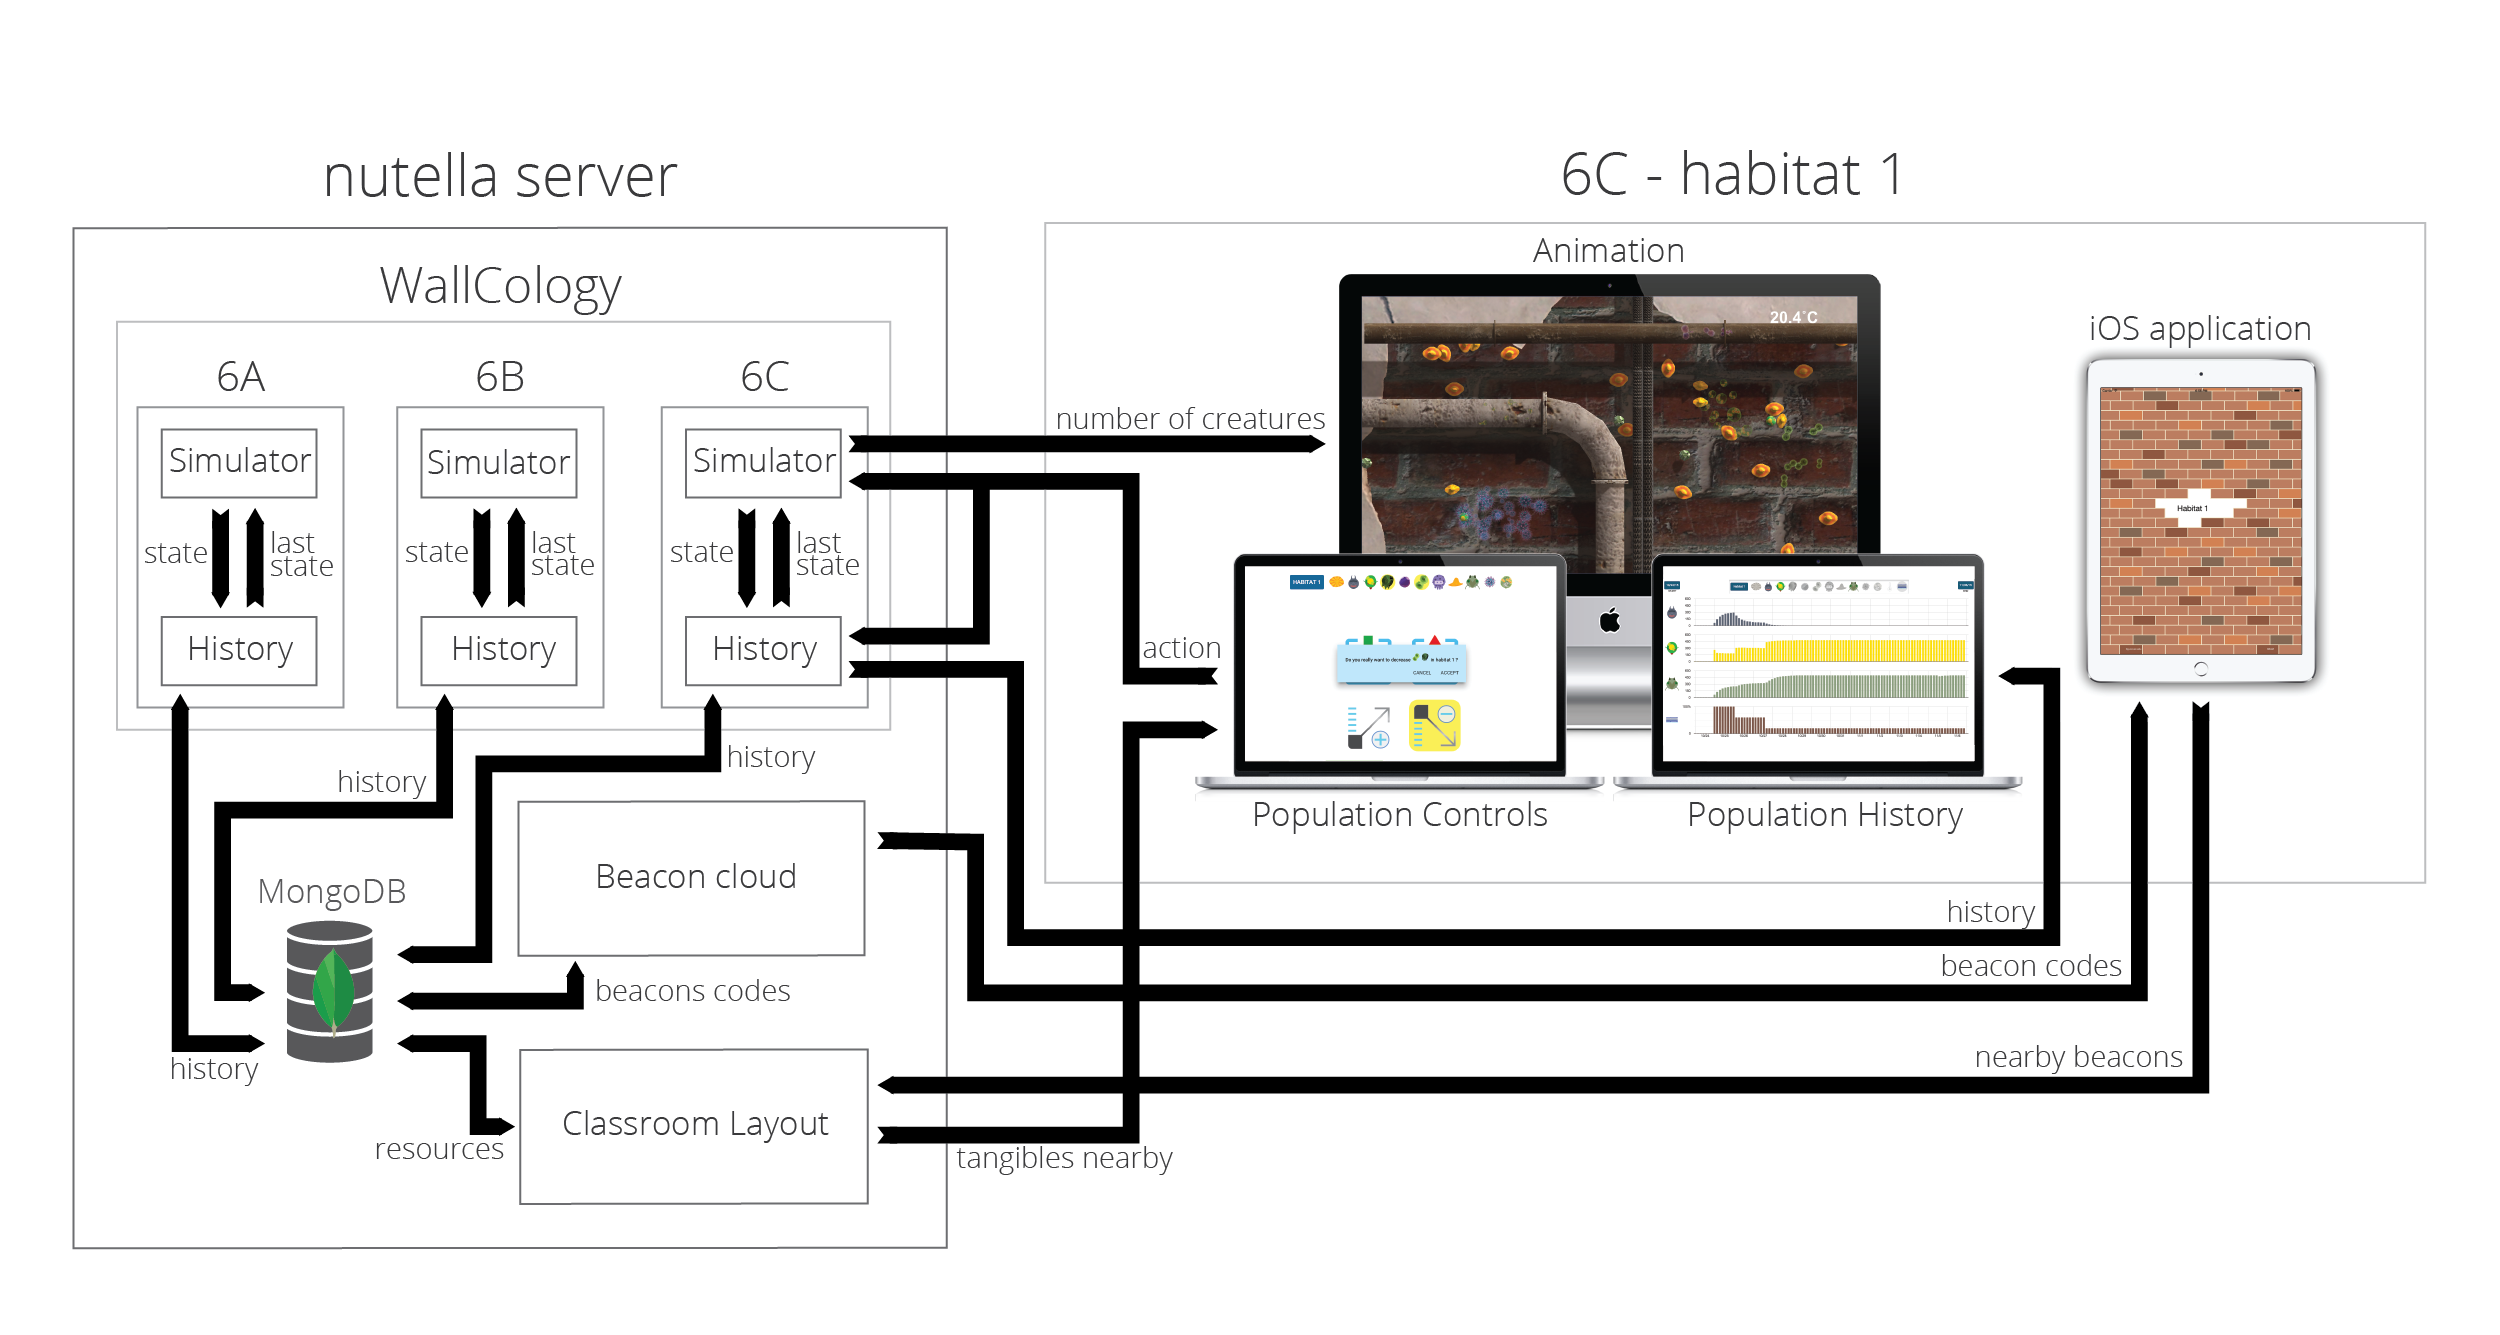
\includegraphics[width=6in]{images/wallcology-structure.png}
\caption{WallCology application structure with all the connections between components}
\label{fig:wallscopes}
\end{figure}

In order to have quantitative information about the species that live inside the walls there's another interface tool called \textit{History Graphs}: it displays how the species populations evolve overtime in a certain habitat. The simulation runs all the time and the changes happen slowly when students are not watching the \textit{Wallscopes} (for example during the night). This tool capture the history of the population that evolve overtime and allows students to explore, for any point in time, how many creatures were in a certain habitat. The tool is shown in \ref{fig:population_history}.

The third interface is the \textit{Population Control} and allow students and teachers to interact and modify the environments, changing the population levels and the habitat variables (like the number of pipes present or the temperature). The interface is visible in \ref{fig:population_controls_unlocked}.
There are four actions allowed on the species:
\begin{itemize}
    \item Increase: increment the creatures of a certain species.
    \item Decrease: reduce the creatures of a certain species.
    \item Insert: inject a new species that was not present before.
    \item Remove: eliminate completely all the elements of a species.
\end{itemize}

There are four actions that can change the habitat:
\begin{itemize}
    \item Temperature increase.
    \item Pipe collapse.
    \item Wall collapse.
    \item Infestation of a foreign species.
\end{itemize}

The environmental actions are reserved for the teacher and the species actions can be executed by students and called \textit{perturbations}. The tangible controls were introduced in order to allow students to execute those actions and the tangible interface is proposed as an alternative to the traditional web interface that was also present. Both the interfaces were explained to children and look exactly the same with the only difference that when tangibles were enabled the cursor on the screen was disabled. This interface employs \textit{RoomPlaces} APIs, implemented in \textit{nutella.location}, in order to check if some tangible is present around the \textit{Wallscopes} (it was decided a threshold distance of 70 centimeters, below it an enter event is dispatched and the interface reacts to that action).

\begin{figure}
\centering
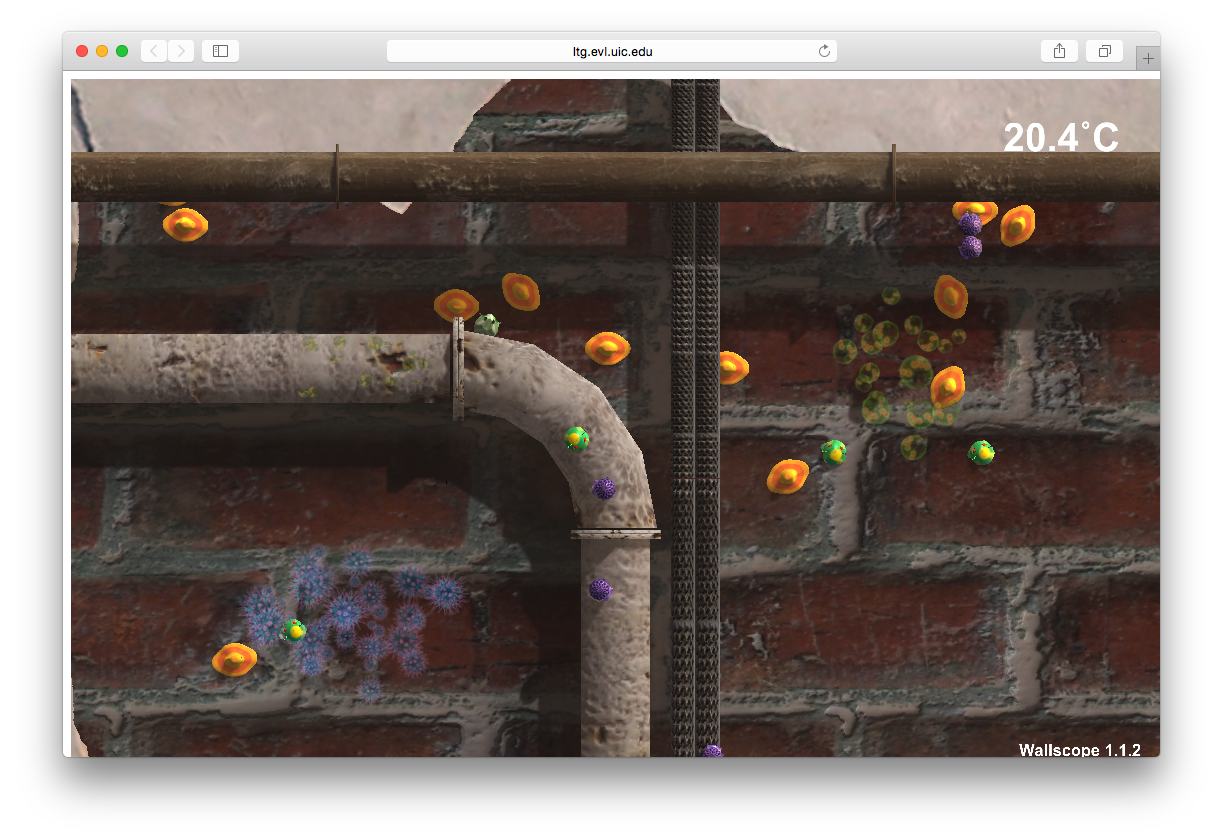
\includegraphics[width=5in]{images/ecosystem-1.png}
\caption{habitat simulation interface that shows a sample of creatures present in the ecosystem. Interactions between creatures are accurate and reflact their role (e.g. predators, herbivores)}
\label{fig:ecosystem_1}
\end{figure}

All the interfaces earlier introduced are nutella interfaces and implemented using nutella library.

\subsection{Hardware components}
Every habitat is a physical place inside the classroom, where is present a computer that represents the WallScope and a tablet that senses if there are tangibles near that habitat. At the beginning of every lesson, they are both started and manually configured for the classroom. In order to do this initial configuration, it was used \textit{RoomCast} software component, that embeds all the functions for selecting the class and the ecosystem number.

Physical tangibles were created using a 3D printer and later painted for representing exactly the creatures inside the simulation.

\subsection{Population controls interface}
\label{subsec:population_control_interface}

The function of this interface is applying perturbations to the habitats. The interface takes the habitat number as parameter and uses it for knowing what is the resource identifier (rid) of the tablet that is tracking tangibles for that habitat. Once the resource identifier is known, the interface invokes the events APIs contained in \textit{nutella.location} module (that provides a push functionality) asking to be notified every time a tangible enters or exits the habitat. The role of \textit{RoomPlaces APIs} is fundamental in this scenario because they allow to decouple the two hardware components, giving advantages compared to a Client-Server model that requires the server to be reliable and willing to accept connections every time. The improvements are:
\begin{itemize}
    \item The interface on the computer and the application on the tablet can be started independently, there's no predefined order.
    \item One of the two components can be replaced real time if necessary (e.g. a tablet out of battery can be replaced with another one) without impacting the second component.
    \item In case of network problems it is sufficient to reconnect the components to Internet.
\end{itemize}

The interface has two states: \textit{locked} (\ref{fig:population_controls_locked}) and \textit{unlocked} (\ref{fig:population_controls_unlocked}). By design this interface doesn't allow any interaction with the mouse and it is unlocked only when a \textit{tangible key} is present near the habitat (detected with the tablet). On the top part of the interface is present the species selector that shows in every moment the species that are selected. On the bottom there are the four actions: insert, remove, increase, decrease. 

In order to execute one action on an habitat at least three tangibles must be detected by the tablet:
\begin{itemize}
    \item Species tangible: one or more species on which execute the action
    \item Action tangible: the action that must be executed on the selected species
    \item Key tangible: unlock the interface
\end{itemize}
Once all those elements are present, a confirmation message is displayed and the action is sent to the simulation bot (using \textit{nutella.net} APIs) that will update the simulation state.

There are a couple of features that are present in the interface and are the result of functionalities provided by RoomPlaces. When the interface is first started, it is unknown if there are tangibles inside the habitat (entering events are sent before the interface starts are lost), for this reason the first action executed during the bootstrap is discovering (using RoomPlaces APIs contained in \textit{nutella.location}) if some tangible is in proximity of the tablet (\textit{pull} functionality). When the key leaves the habitat, the interface is automatically locked and the species and actions automatically deselected and when it re-enters the habitat the pull functionality is used again in order to check which species and action to select. It is important to highlight that every time the push functionality is used the result is instantly returned without asking the server, this mechanism speeds up the interface and creates a better user experience. During the activity, this interface was improved in order to prevent some type of error that students committed in the early lessons. A confirmation message was added when an action was executed on the server, this message is useful for being sure that the server is still working (no crash occurred) and is useful for the students because they can be sure that the action is registered in the system.

\begin{figure}
\centering
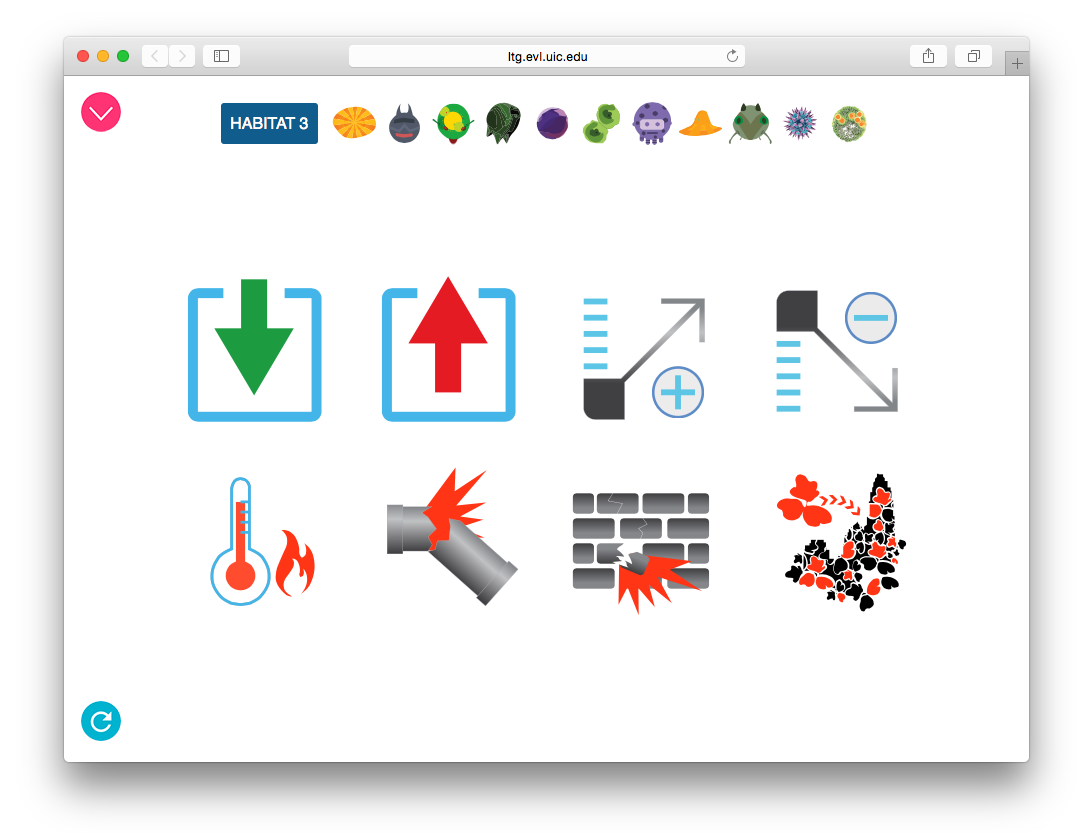
\includegraphics[width=4.5in]{images/population-controls-teacher.png}
\caption{complete population controls interface for teachers}
\label{fig:population_controls_teachers}
\end{figure}

\begin{figure}
\centering
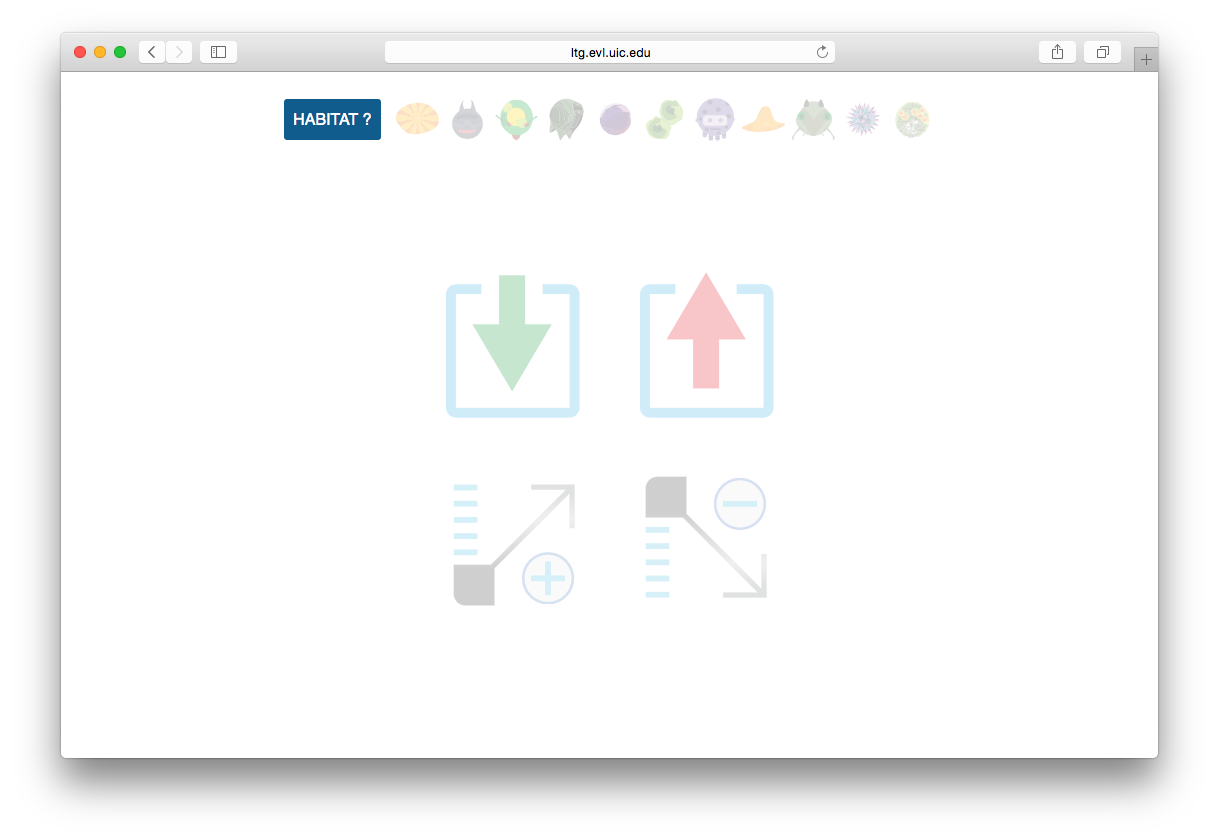
\includegraphics[width=4.5in]{images/population-controls-locked.png}
\caption{population controls interface locked}
\label{fig:population_controls_locked}
\end{figure}

\begin{figure}
\centering
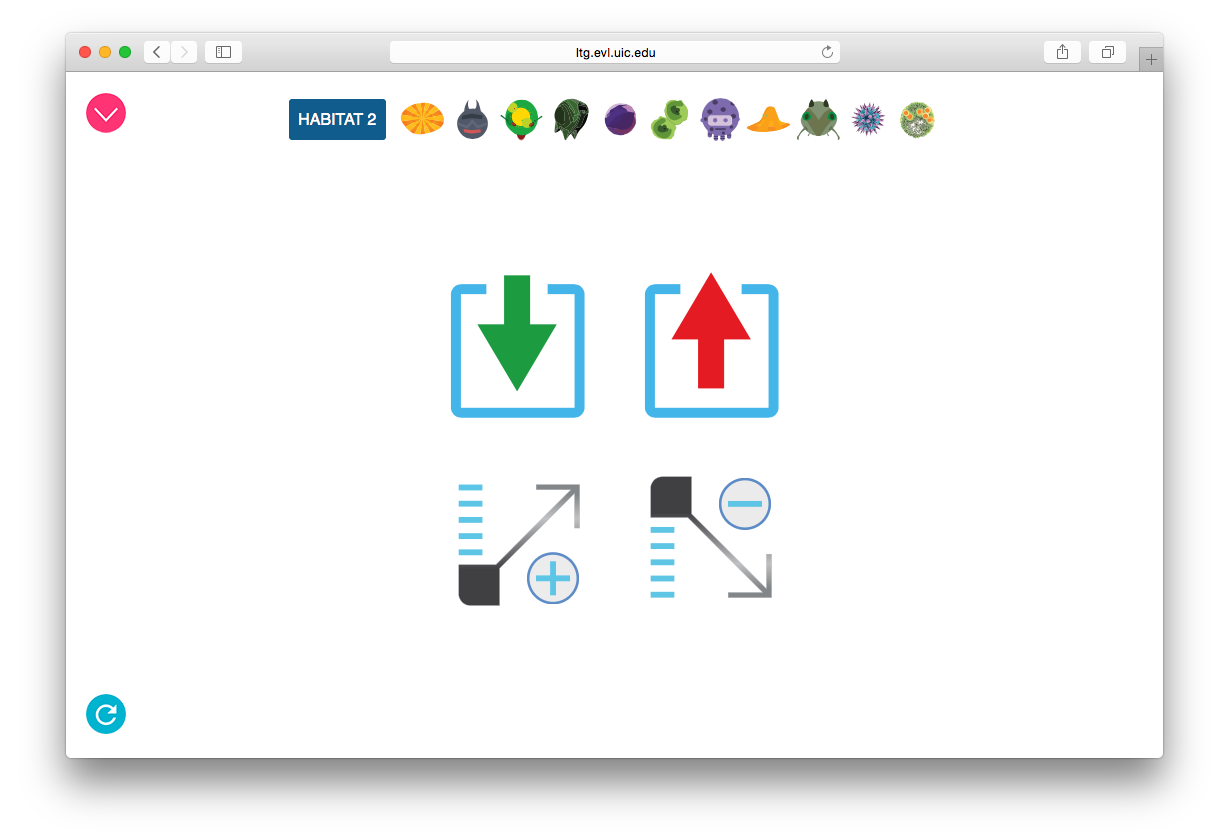
\includegraphics[width=4.5in]{images/population-controls-unlocked.png}
\caption{population controls interface unlocked}
\label{fig:population_controls_unlocked}
\end{figure}

\begin{figure}
\centering
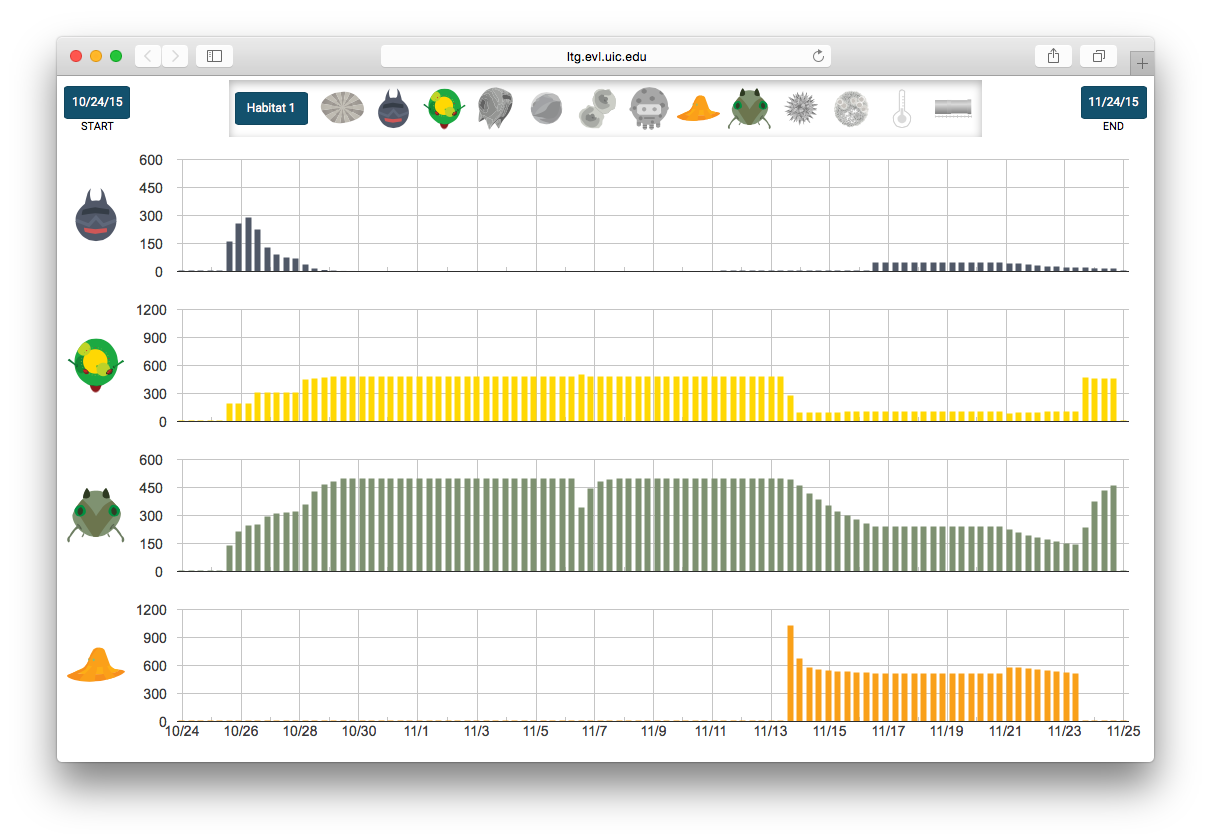
\includegraphics[width=4.5in]{images/population-history.png}
\caption{population history tool}
\label{fig:population_history}
\end{figure}

\subsection{RoomPlaces configuration}
In order to provide the best user experience possible, it is necessary to hide all the technical details about how tangibles work, at the point in which the user cannot feel that they contain an electronic device while using them. In order to do it, I took advantage of the different levels of abstraction between the hardware device (the iBeacon) and the \textit{population controls} interface. In the next paragraphs I describe those abstractions and why they are important.

The first abstraction layer is provided by \textit{Beacon Cloud}. Every beacon used in the study was manually inserted in the list (only once when it was purchased) and an human readable name was assigned to it. It is possible to see a list of beacons in \ref{fig:wallcology_beacon_cloud}. This abstraction is important because iBeacons have three identifiers that are too long to be remembered (they're long because every beacon must be unique in the world), associating a human readable name considerably increase the usability of \textit{Classroom Layout} interface minimizing the errors end the time during the developing phase.

\begin{figure}
\centering
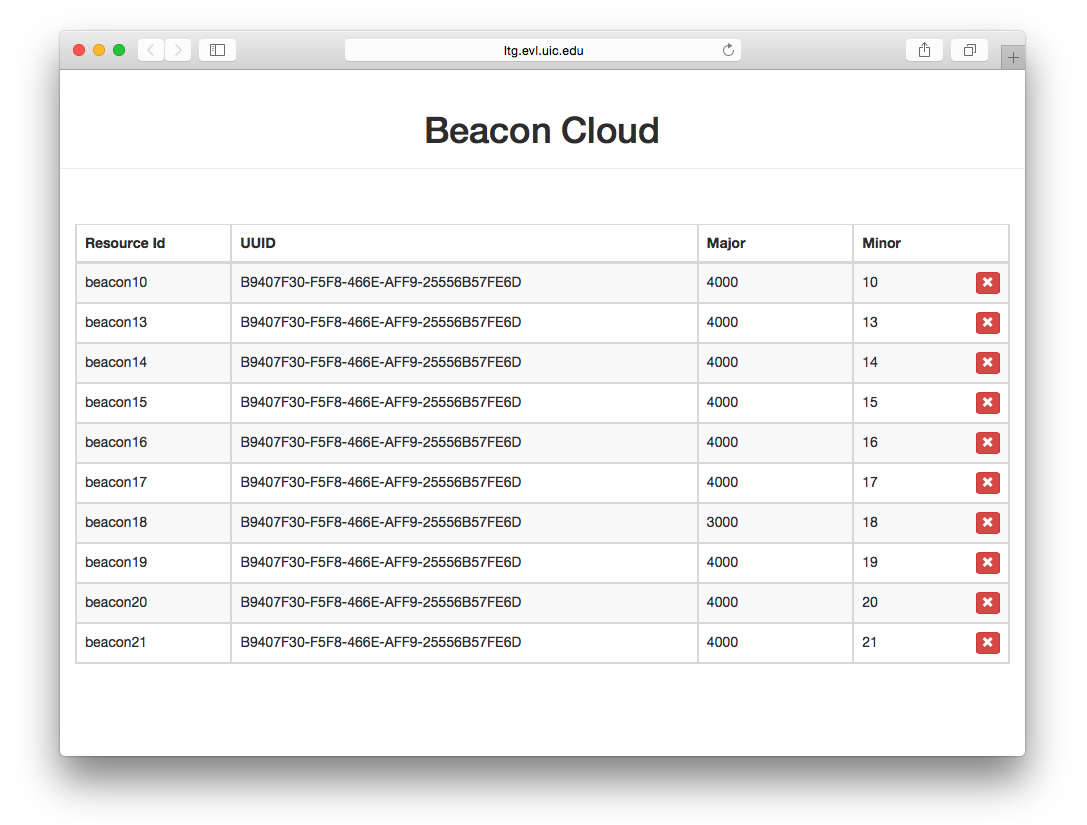
\includegraphics[width=4.5in]{images/wallcology-beacon-cloud.png}
\caption{Beacon Cloud configuration phase}
\label{fig:wallcology_beacon_cloud}
\end{figure}

The second layer of abstraction is provided by \textit{Classroom Layout} component: all the beacons are inserted in automatic \textit{proximity} tracking mode, and for every beacon, additional information was associated to it: the role (key, action or species) and an alphanumeric identifier (the species index or the action name). This abstraction is particularly useful in case of hardware failure of beacons (that can happen due to the battery depletion): it introduces redundancy because the same role can be assigned to more than one beacon and if the first one fails it can be quickly replaced. \textit{Population control} interface has only to look at the "role" data associated with the object and to "key", "action" or "species" data for discovering all the information about the tangible, without the need to hard-code beacon identifiers in the interface. During the Classroom Layout configuration, 19 \textit{tangibles} were introduced as dynamic resources (11 species, 4 actions and 4 keys) and 4 \textit{Wallscopes} as static resources (able to track the dynamic resources) with a proximity radius of 70 centimeters. This configuration was repeated for all the three classes.

\begin{figure}
\centering
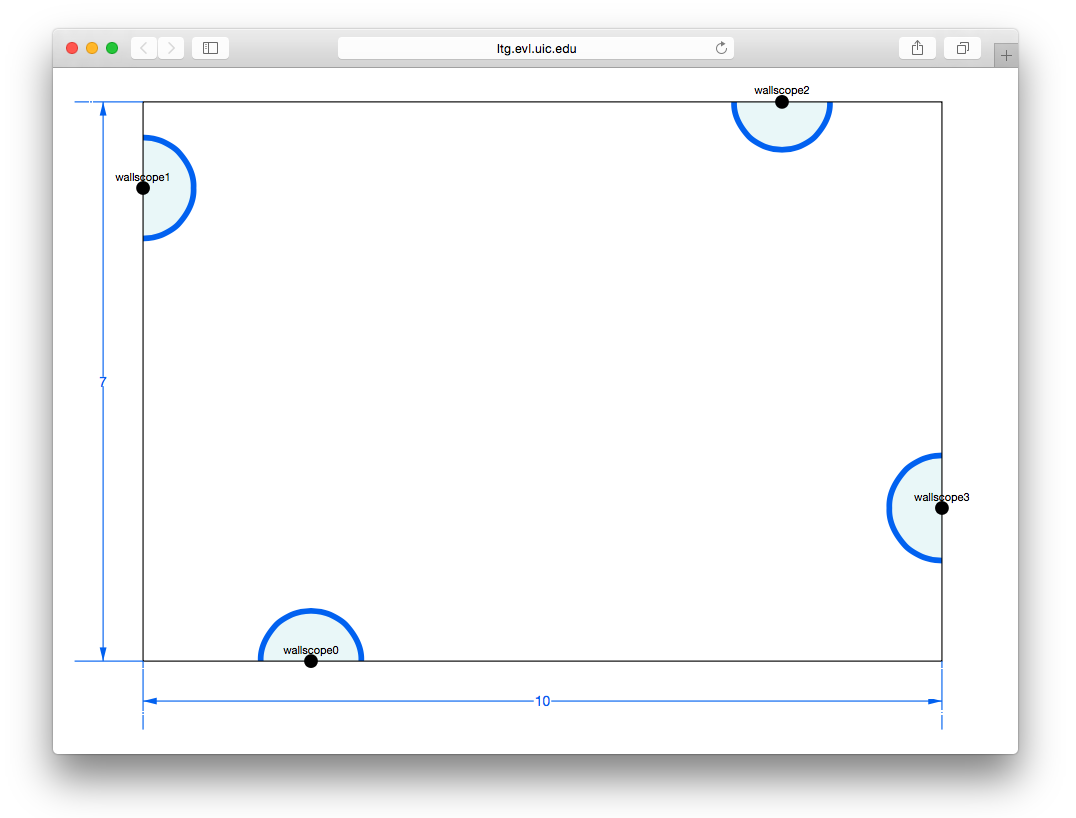
\includegraphics[width=4.5in]{images/wallcology-classroom-layout.png}
\caption{population controls interface unlocked}
\label{fig:wallcology_classroom_layout}
\end{figure}

The last action that enabled the integration of tangibles is initializing \textit{nutella.location} module (RoomPlaces APIs) inside \textit{population control} interface with the right wallscope resource identifier in order to virtually connect the tablet to the \textit{population control} interface.

\subsection{Wallcology iPad application}
It is a simple application that uses the \textit{nutella.location} module encapsulated in an iOS framework in order to be easy to integrate in an iOS application written in Swift. The application displays a simple user interface that allows to choose the class name and the identifier to use (\textit{Wallscope} index).

Even if this application was very easy to write and deploy, it is the core of the \textit{RoomPlaces} mechanism and everything that happen behind the scenes is encoded in the nutella.location module integrated in nutella\_lib.swift \cite{nutella_lib_swift}. The application communicates with Beacon Cloud and downloads all the information about beacons. When it has the list, starts sensing for every beacon around it and in case iOS discovers some one of them, reports the \textit{resource identifier} to \textit{Classroom Layout} bot that knows the configuration of the classroom and can decide if a proximity event must be dispatched.

\begin{figure}
\centering
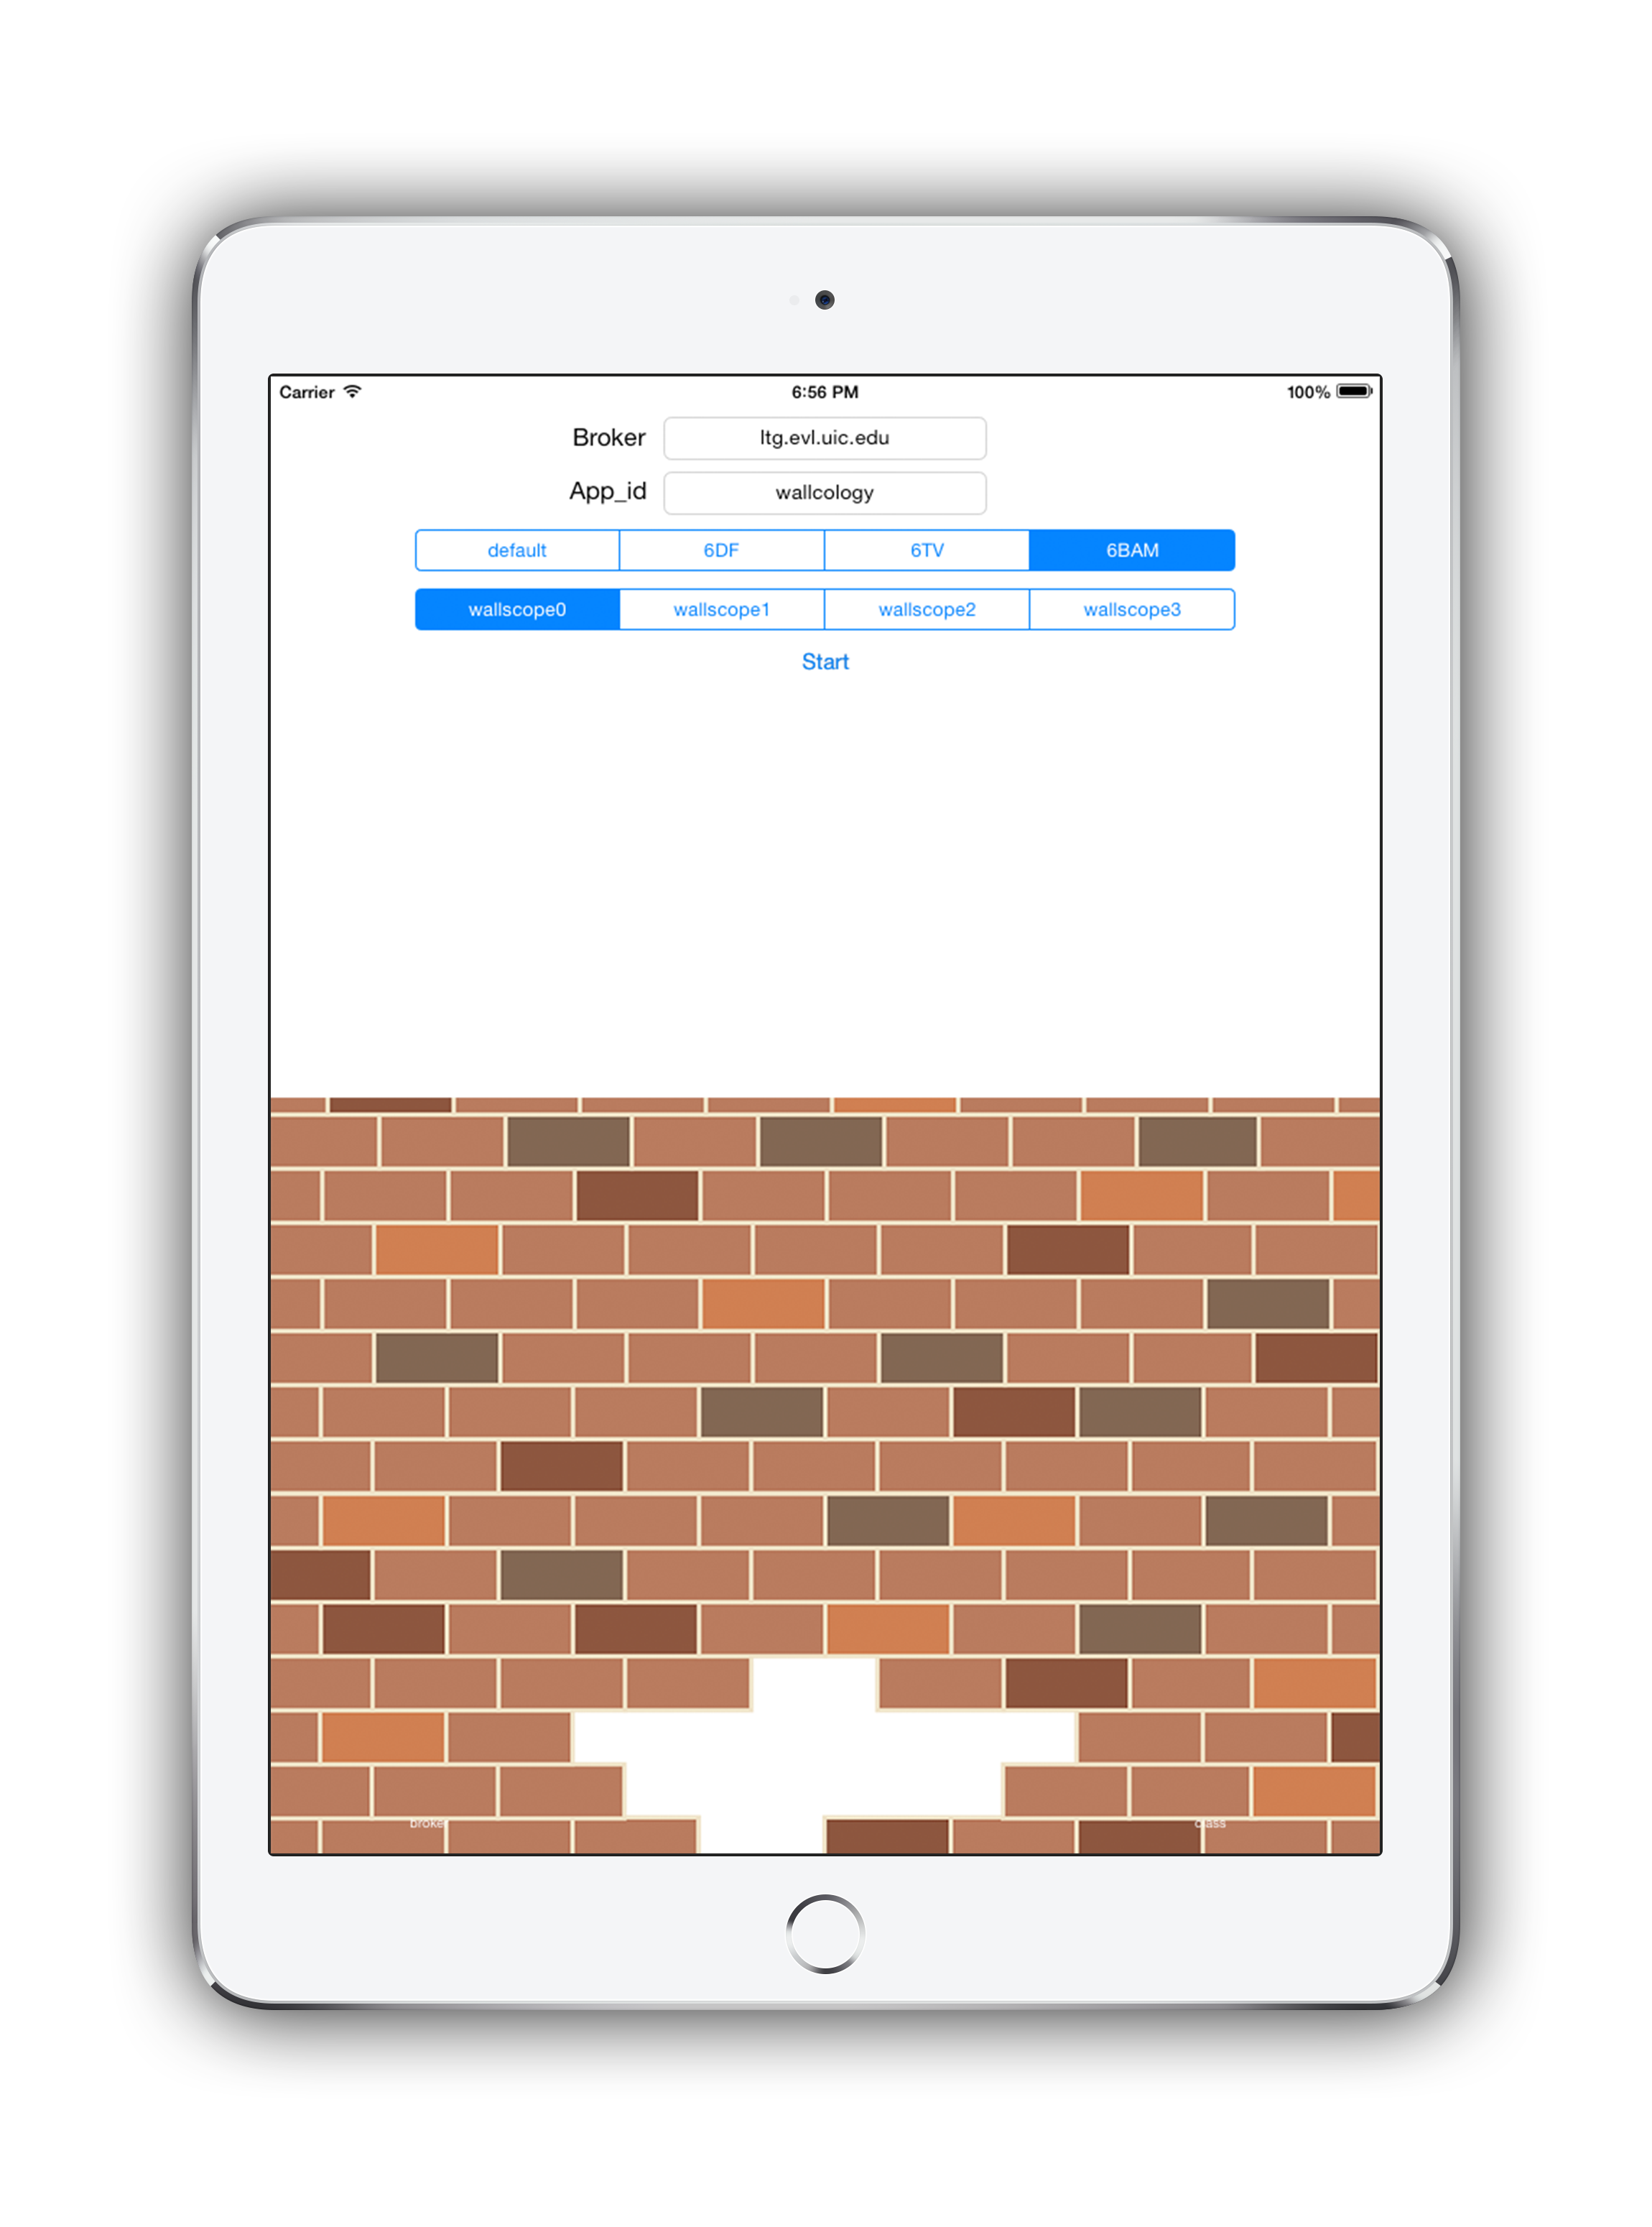
\includegraphics[width=3in]{images/wallcology-ios.png}
\caption{iOS application configuration phase}
\label{fig:wallcology_ios_config}
\end{figure}

\begin{figure}
\centering
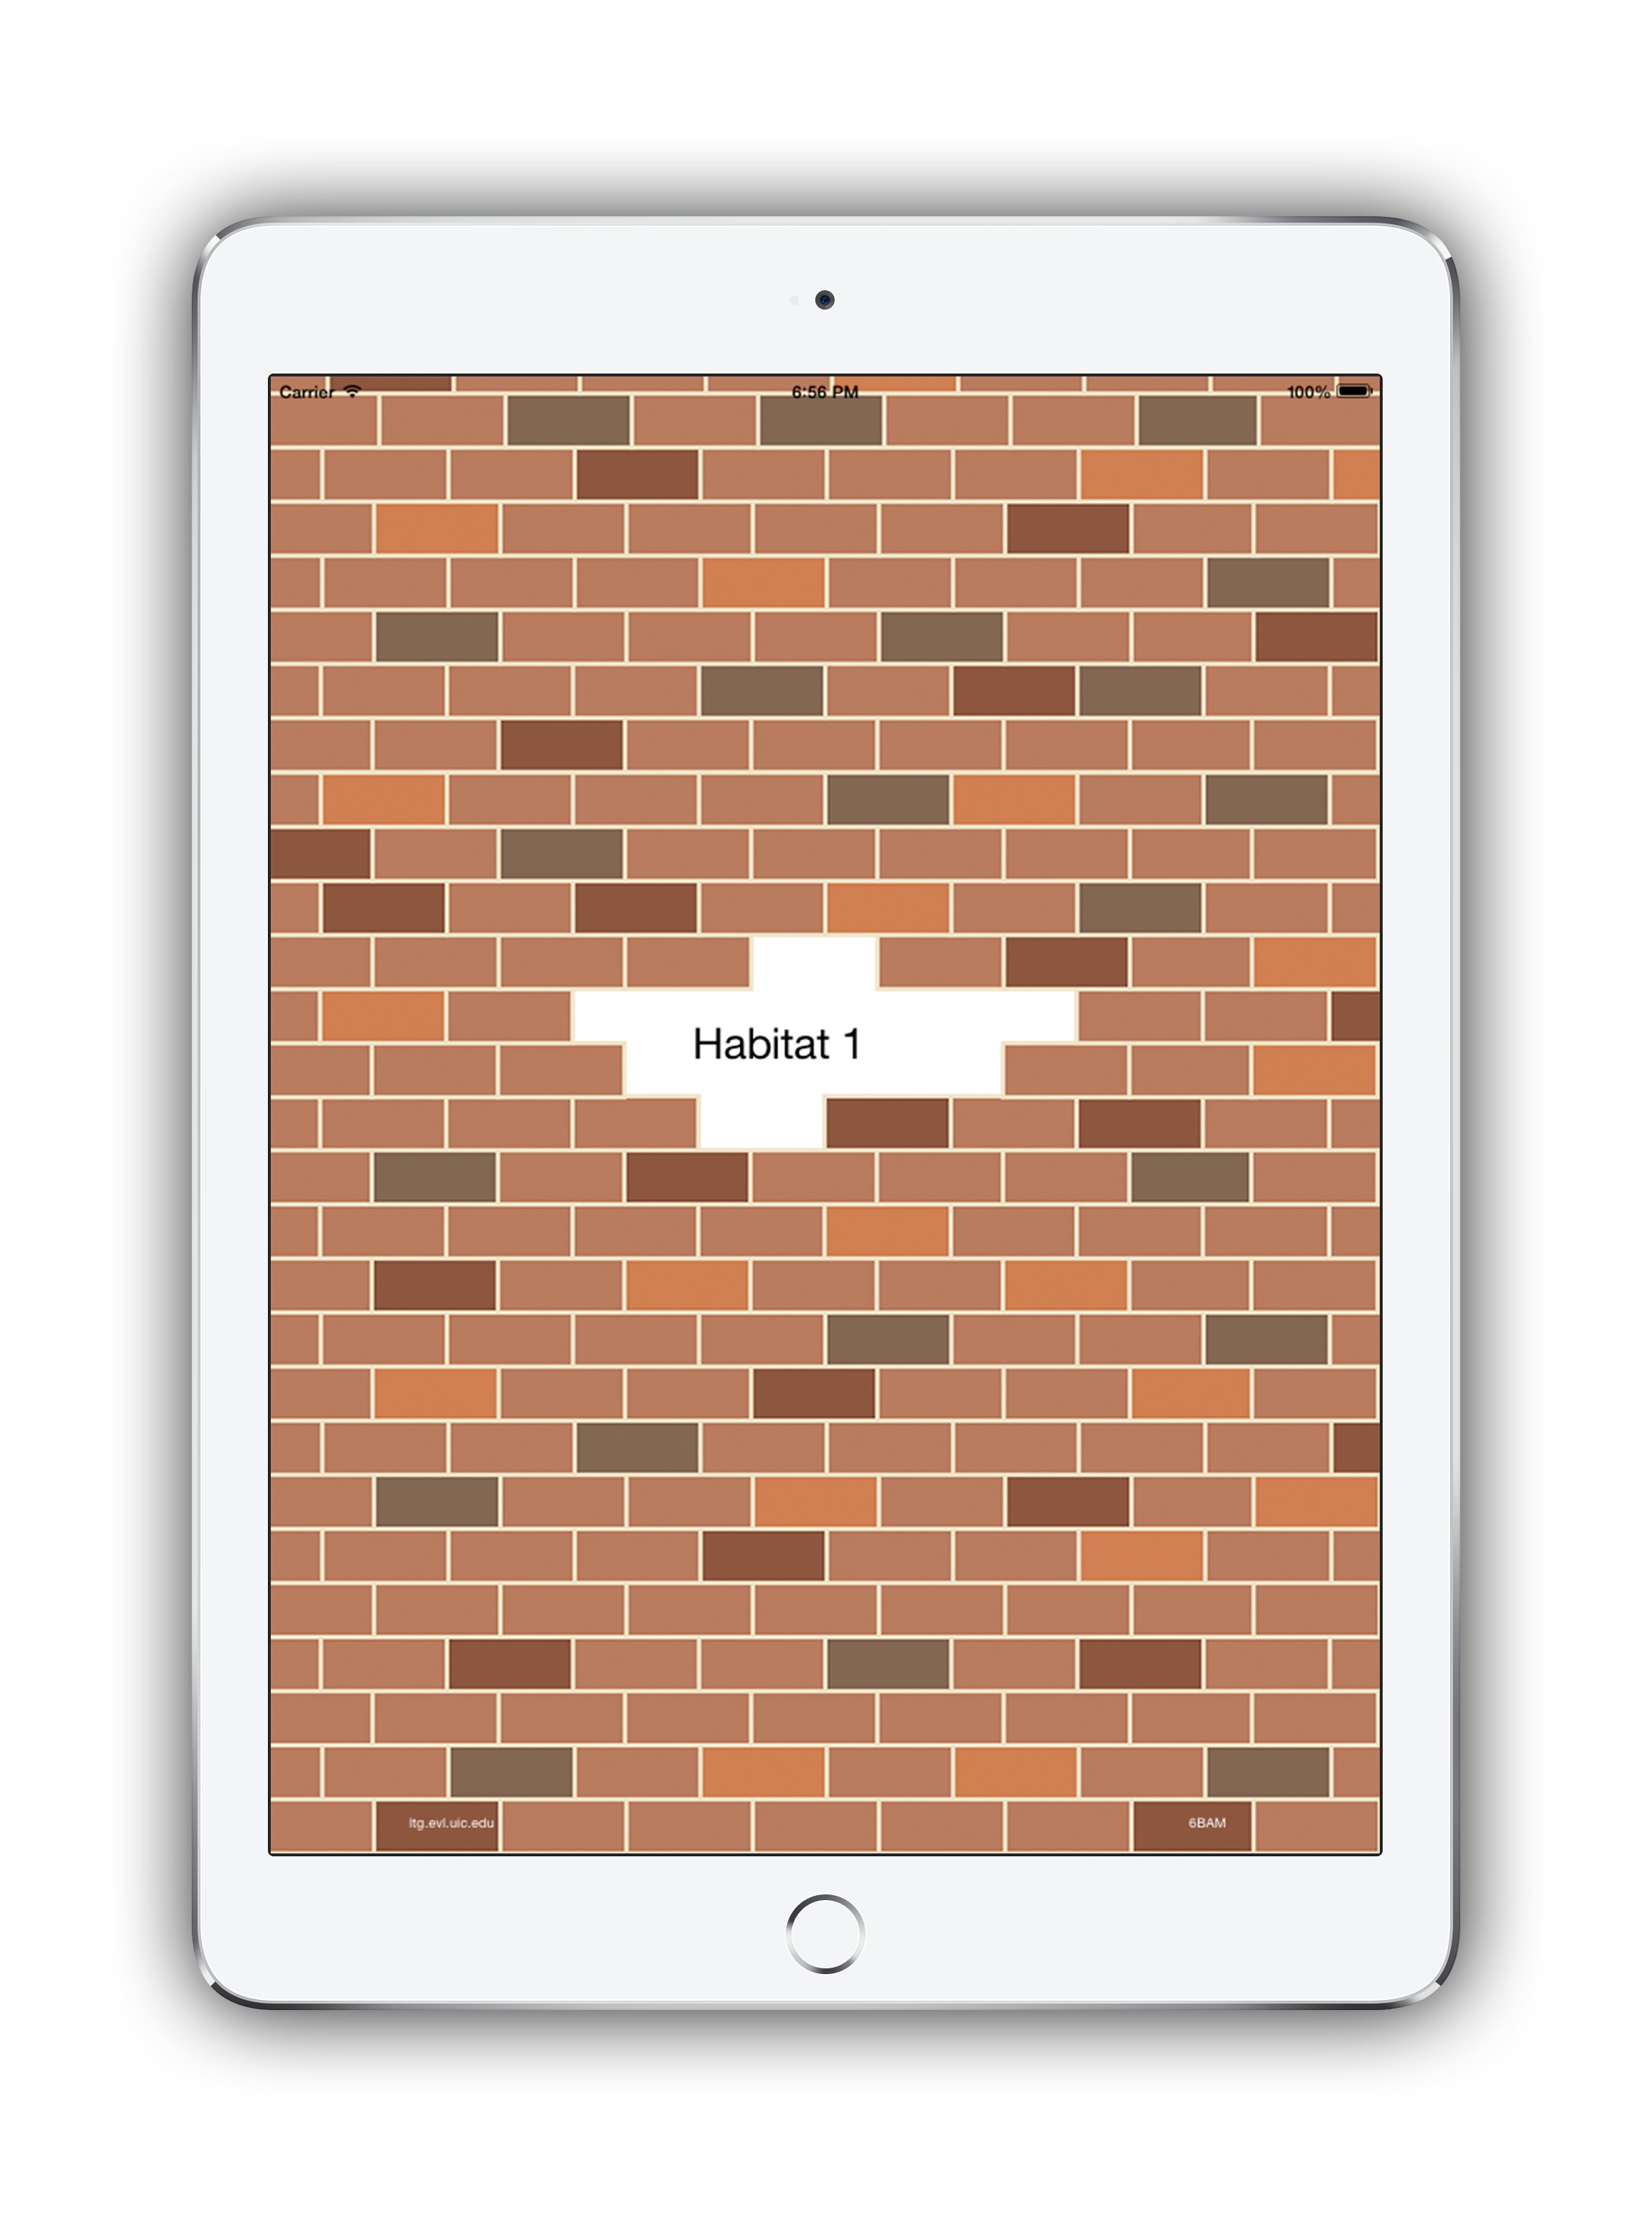
\includegraphics[width=3in]{images/wallcology-ios-sensing.png}
\caption{iOS application while sensing for tangibles}
\label{fig:wallcology_ios_config_sensing}
\end{figure}

\subsection{Simulator bot}
The \textit{Simulator bot} is the component that is in charge to maintain an always running simulation of the ecosystems. There is one instance of this bot for every class. Nutella framework manages when the instances have to start and stop and also the data separation.

This bot has two functions:
\begin{itemize}
\item Update the simulation state every 15 minutes and notify all the components that a change happened.
\item Listen for events coming from \textit{Population Controls} interface and update the state consequently.
\end{itemize}

The simulation state contains the number of creatures of a certain species that are present in every habitat in the present time and also three environmental variables: temperature, pipes level and brick area.

When this bot starts, it requests the last state to the \textit{History bot} and starts the calculations for determining the next state from it. The relations between species (plants, herbivores, predators) are represented using non-linear discrete dynamic systems. This model is stable in certain ranges of temperatures, pipes and bricks area, this will ensure that the effect of every \textit{increase} and \textit{decrease} action will disappear after a certain time and that \textit{insert} and \textit{remove} actions will not generate physically unrealistic behaviors (negative or too many individuals of certain species). At every iteration (every fifteen minutes) a set of equations is used to recalculate the populations living in the ecosystems.

\subsection{History bot}
This bot has the only purpose of listening for state changes and perturbations (on the habitat and on the species) and write them in a persistent object that acts as an hystorical log of everythong happened in the simulation (both the automatic behaviors and the user interactions).

It is possible, in every moment, to query the bot for retrieving the history. \textit{Population History} interface requests this bot for information about the population. It is also used in order to recover \textit{Simulator} bot after a crash or during the normal start-up procedure.

\subsection{RoomCast}
In order to provide classrooms isolation, every component that contains \textit{nutella.lib} needs to know the class identifier (for convention the name of the class was used) and other technical details like the url of the server that hosts the simulation. The bots are entirely managed by \textit{nutella framework} that automatically instantiates all of them providing these parameters automatically behind the scenes when the new run is spawned with \textit{nutella start} command. On the front-end part, where all the interfaces live (inside a browser), it is not possible to automatically provide all the information needed by nutella (run\_id, app\_id, mqtt\_broker\_address). This problem is even more complicated, by the fact that every interface needs also other information (e.g. the habitat that it must be displayed on that specific computer of the class). By design all those information is concentrated in only one point: the url of the interface. This choice allow to debug the application simply opening an url in the browser. The drawback is that every time students need the tool a very long url must be manually inserted. This problem could be solved with browser bookmarks, but with a very bad user experience while passing form one interface to another. It also had required a lot of manual work because every link must be manually inserted (not a very scalable solution).

In order to simplify the setup of the ecosystems in the three classes it was created a sophisticated environment for providing all the tools in only one web page and allow the students to easily switch from one interface to another without changing browser window, this tool is called RoomCast. In this section I describe the RoomCast parts that were useful during the study.

\begin{figure}
\centering
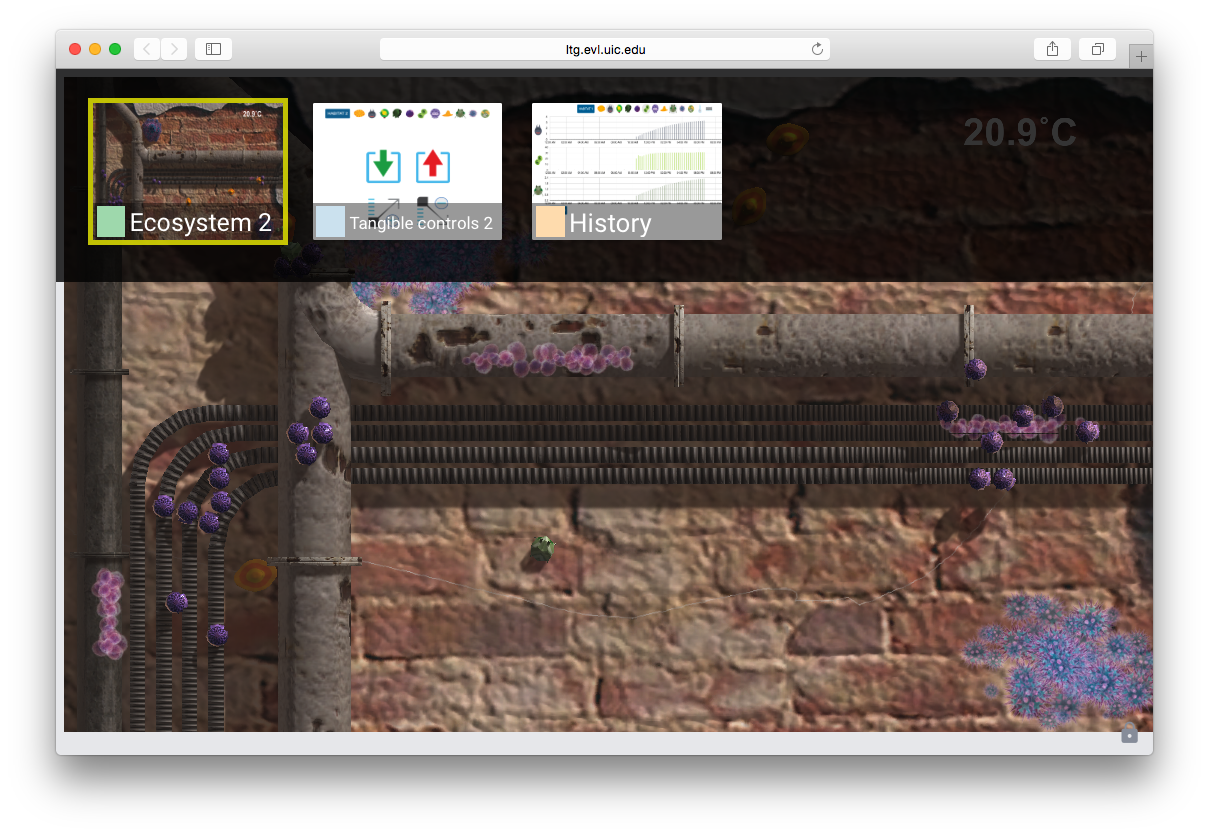
\includegraphics[width=4.5in]{images/room-cast-menu.png}
\caption{RoomCast menu for selecting the interface}
\label{fig:roomcast_menu}
\end{figure}

RoomCast is an interface that wraps all the other nutella interfaces and has the following functionalities:
\begin{itemize}
\item Provides a menu for switching from the current interface to another (\ref{fig:roomcast_menu}).
\item Provides an authentication method that allow to select the classroom and the ecosystem number (\ref{fig:roomcast_classroom}).
\item Provides a teacher interface that is used for controlling which tools are available (\ref{fig:roomcast_role}).
\end{itemize}
The authentication function is important for allowing only the right functions on the specified computer. At the beginning of every lessons, the browser starts automatically on every computer in full-screen mode and the only action required by the teacher is clicking on the name of the current class and current habitat. From that moment on all the interfaces are automatically personalized (the parameters are passed to the interfaces and the url is hidden from the user).

In order to select an interface, the students can click on the pink button present in the top left corner (\ref{fig:population_controls_locked}) of the screen (it can be also moved) in order to show the menu with all the enabled interfaces. In order to control software anomalies in the interfaces a reload button is inserted (blue button in \ref{fig:population_controls_locked}), the button reloads only the current interface without requiring all the others to update. It can also be activated remotely without the user intervention.

\begin{figure}
\centering
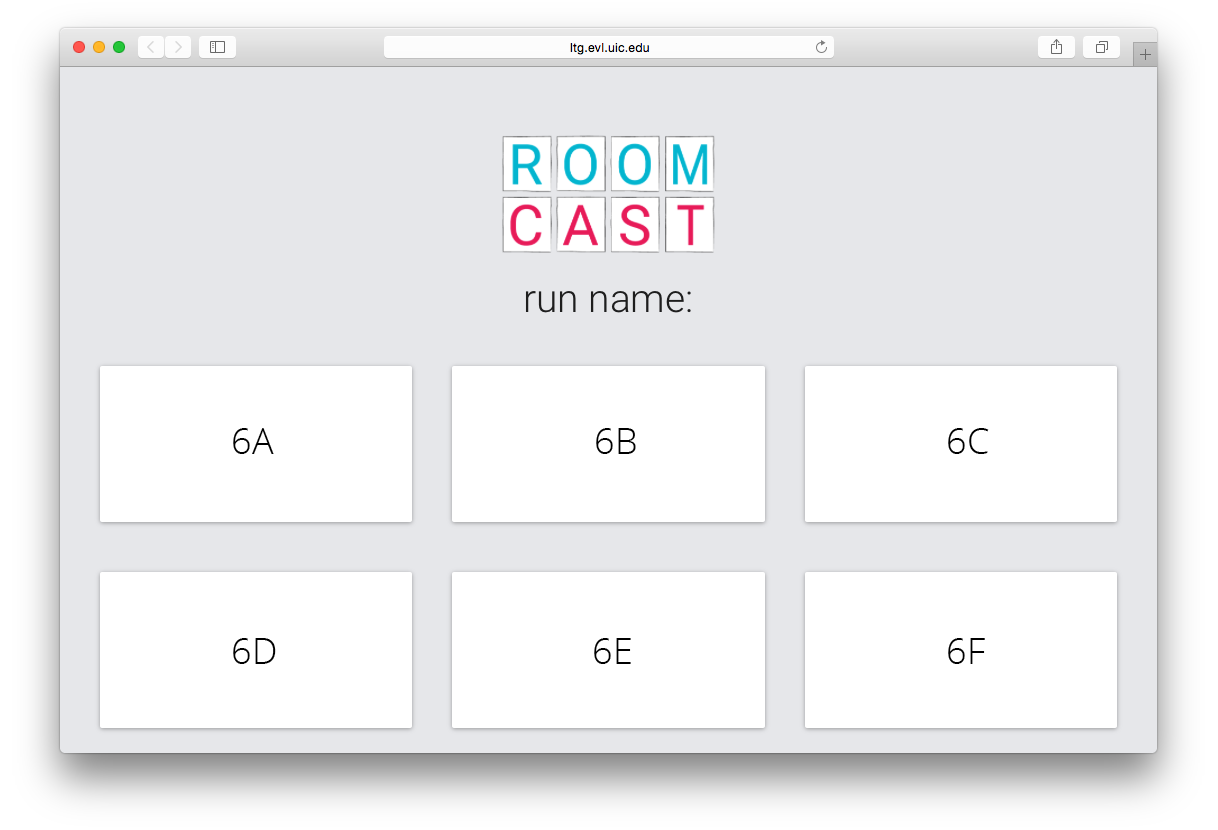
\includegraphics[width=4.5in]{images/room-cast-classroom-selection.png}
\caption{RoomCast interface for the selection of the class}
\label{fig:roomcast_classroom}
\end{figure}

\begin{figure}
\centering
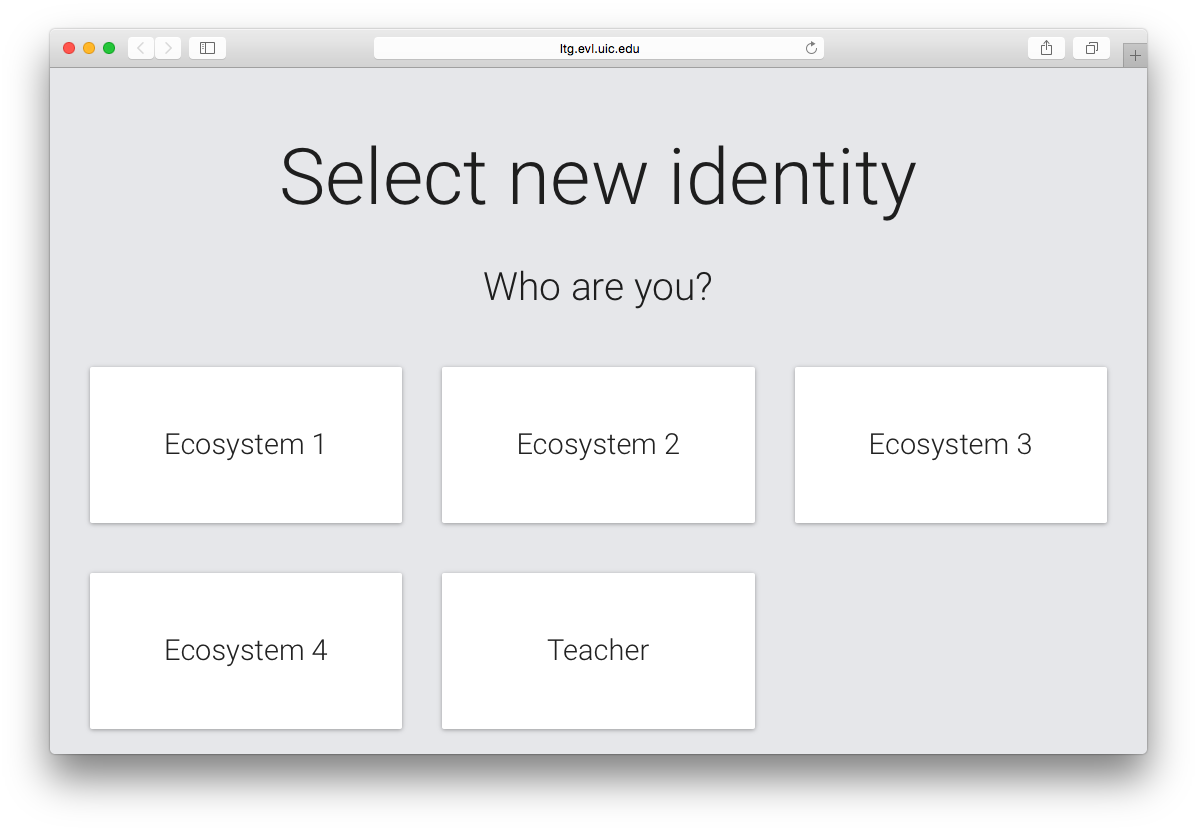
\includegraphics[width=4.5in]{images/room-cast-habitat-selection.png}
\caption{RoomCast interface for the selection of the role (ecosystem number or teacher)}
\label{fig:roomcast_role}
\end{figure}

\section{Research method and data sources}
For answering the research questions, I decided to study children behavior during the class activities that involve the usage of beacons: those activities are called \textit{perturbations} because they modify (\textit{perturb}) the habitat in a number of different ways through the \textit{population control} interface (already explained at the beginning of this section).

The experiment was conducted on three classes of primary school and with a total of 48 children. Two physical room were used: one spacious science laboratory with four desktop computers, positioned on the four walls and one classroom in which four laptops were positioned before the beginning of every lesson. The metaphor used in this study is that every computer is an habitat, a group of four students is assigned to every habitat.

Three different data sources were used for collecting evidence:
\begin{itemize}
    \item Video recordings, simultaneously from four cameras:
    \begin{itemize}
        \item A fixed camera on the ceiling pointing at habitat 1.
        \item A fixed camera on a shelf capturing the entire room.
        \item A moving camera on a tripod, always filming the current activity and the center of attention of the class.
        \item A smartphone camera operated by a researcher, activated when discussion happen inside a student group
    \end{itemize}
    \item Questionnaire for children with 5 questions asking different aspects of the interaction with tangibles
    \item Software interface action logging
\end{itemize}

The two fixed cameras were used only in the science laboratory because it was the only place where the computer remained in the same position all the time, in the other classroom the laptops moved every lesson and also during the activities. 

A major challenge that video recordings presented was the collection of evidence of discourses between students about the scientific topic. The task was difficult because they happened in different areas of the class simultaneously between 16 students and it was not easy to predict the best place to record with the moving cameras. The method applied was to continuously film one habitat with a fixed camera recording everything happened there. Use a shelf mounted fixed camera without audio for recording all student-to-student interactions for distinguishing when they happen between students of the same group or between students of different groups. Use the smartphone camera and a tripod mounted camera for capturing single discourses taking place near the researcher and moving rapidly from one group to the others in order to capture the maximum number of conversations.

The questionnaire was assigned to the students to complete after they tried both the web interface and the tangibles in order to make a perturbation. The web interface and the tangible interface show exactly the same elements on the screen, with the only difference that when the tangibles were enabled students could not use the mouse for interacting (except for confirming the action).

The last data collection method is based on writing a log (on the server using nutella capabilities) that records every time which interface is used for doing the perturbation (tangibles or web interface), on which habitat is done and who does it (the teacher or the students). This method is not really useful because at the beginning of each lecture the teacher forced the students to use one interface or the other, but is a confirmation for us that the system is working and provides information on what really happened. The teacher interface was entirely operated by me in order to change habitats conditions. Sometimes certain groups discussed longer than others and didn't have time to do the perturbation during the lecture. The teacher interface was also used in order to change the amount of pipes present in some ecosystems that is an action that students are not allowed to do.

\subsection{Tangibles creation and RoomPlaces integration}
Tangibles are the interface that children have the opportunity to use and that are subject of this study. For this reason a huge amount of time was invested in order to design and build solid, pleasant and funny creatures that have the possibility to became valuable practice-linked resources and possibly cultural artifact \cite{horn:role}. During the design phase three elements were kept into account:
\begin{itemize}
\item Possibility of embedding an iBeacon sensor inside them
\item High fidelity of the final result with the 3D model present in the animation
\item High quality of the final result in term of robustness and impact resistance 
\end{itemize}

The design phase is divided in two parts: the design of the iBeacon container and the design of the creatures. During both the phases Maya 3D modeling software was employed. The first phase required to measure the beacon size and to create a cavity inside a base that was used to contain the Bluetooth LE emitter. The second phase took more time because it required to model all the creatures, it was done only once for both creating the simulation and the tangibles.

The 3D models were created with a 3D printer. The chosen material was tested against Bluetooth signal attenuation. They were painted in order to replicate the exact same texture of the creatures in the simulation and glued with the base where the iBeacon was inserted. The final result is shown in \ref{fig:tangibles}. For the other tangibles: 4 species, 4 actions and 4 keys the graphic icons were printed, laminated and glued on the beacon base.

\begin{figure}
\centering
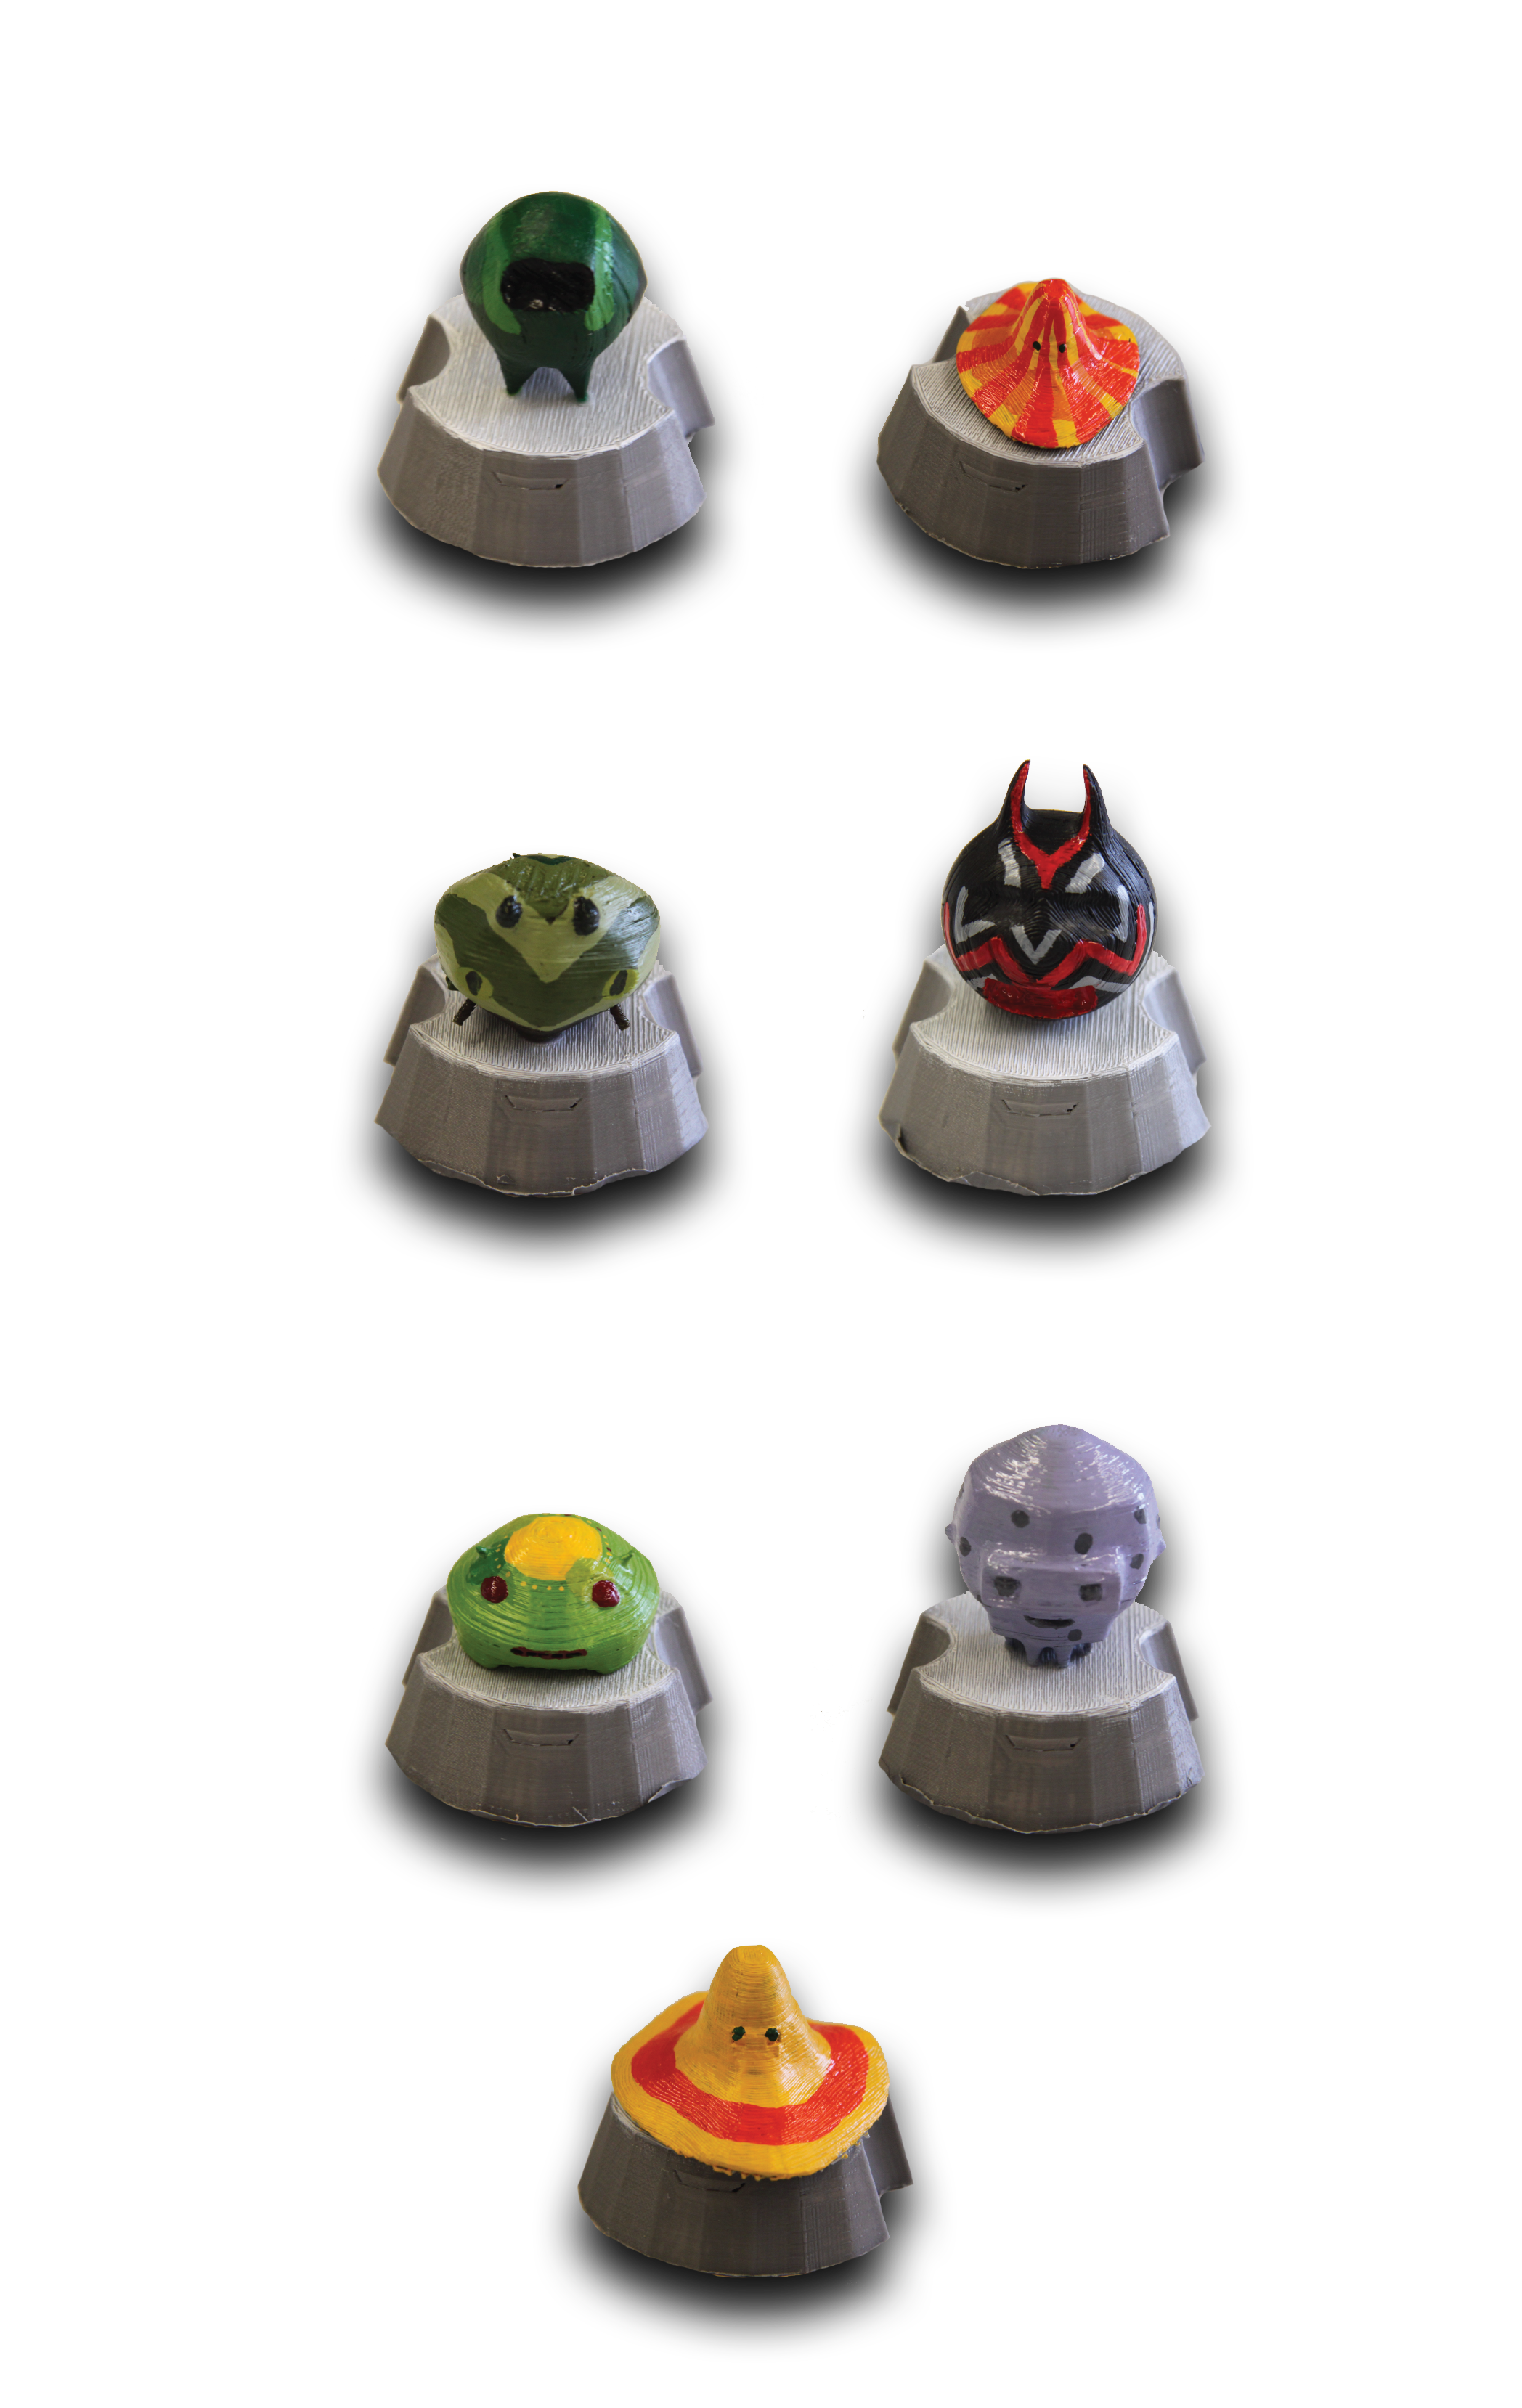
\includegraphics[width=5in]{images/tangibles.png}
\caption{seven creature tangibles printed in 3D}
\label{fig:tangibles}
\end{figure}

Every tangible contains exactly one beacon that was previously registered in the system using the \textit{Beacon Cloud} interface and inserted in every class using \textit{Classroom Layout} interface. In order to simplify the substitution of the beacons (inside tangibles), in case of hardware failure, the \textit{resource identifier} of the beacon is  printed on the bottom of the base.

\section{Results}
In this section I report the results of the exploratory study and I give answers to the research questions supported by evidence that I collected using the data sources.

\subsection{Tangibles improve children enjoyment}
In this story, I support with evidence my expectation that tangibles can improve the quality of the lectures, engaging students in funny activities, stimulating their curiosity and letting them focus better on the topic keeping high the motivation.

During the study, in order to develop a personal connection with the creatures, teachers let students chose the names (reported in \ref{tab:species_names}). Every class chose different names for the species and many students had the opportunity to personally assign the names. There are evidence in the video that show how children are excited when they play with the creature they named.

\begin{table}
\centering
\begin{tabular}{ | c | c | c | c | c | }
\hline
Species   & Icon & Name 6A & Name 6B & Name 6C \\
\hline
Species 0  & 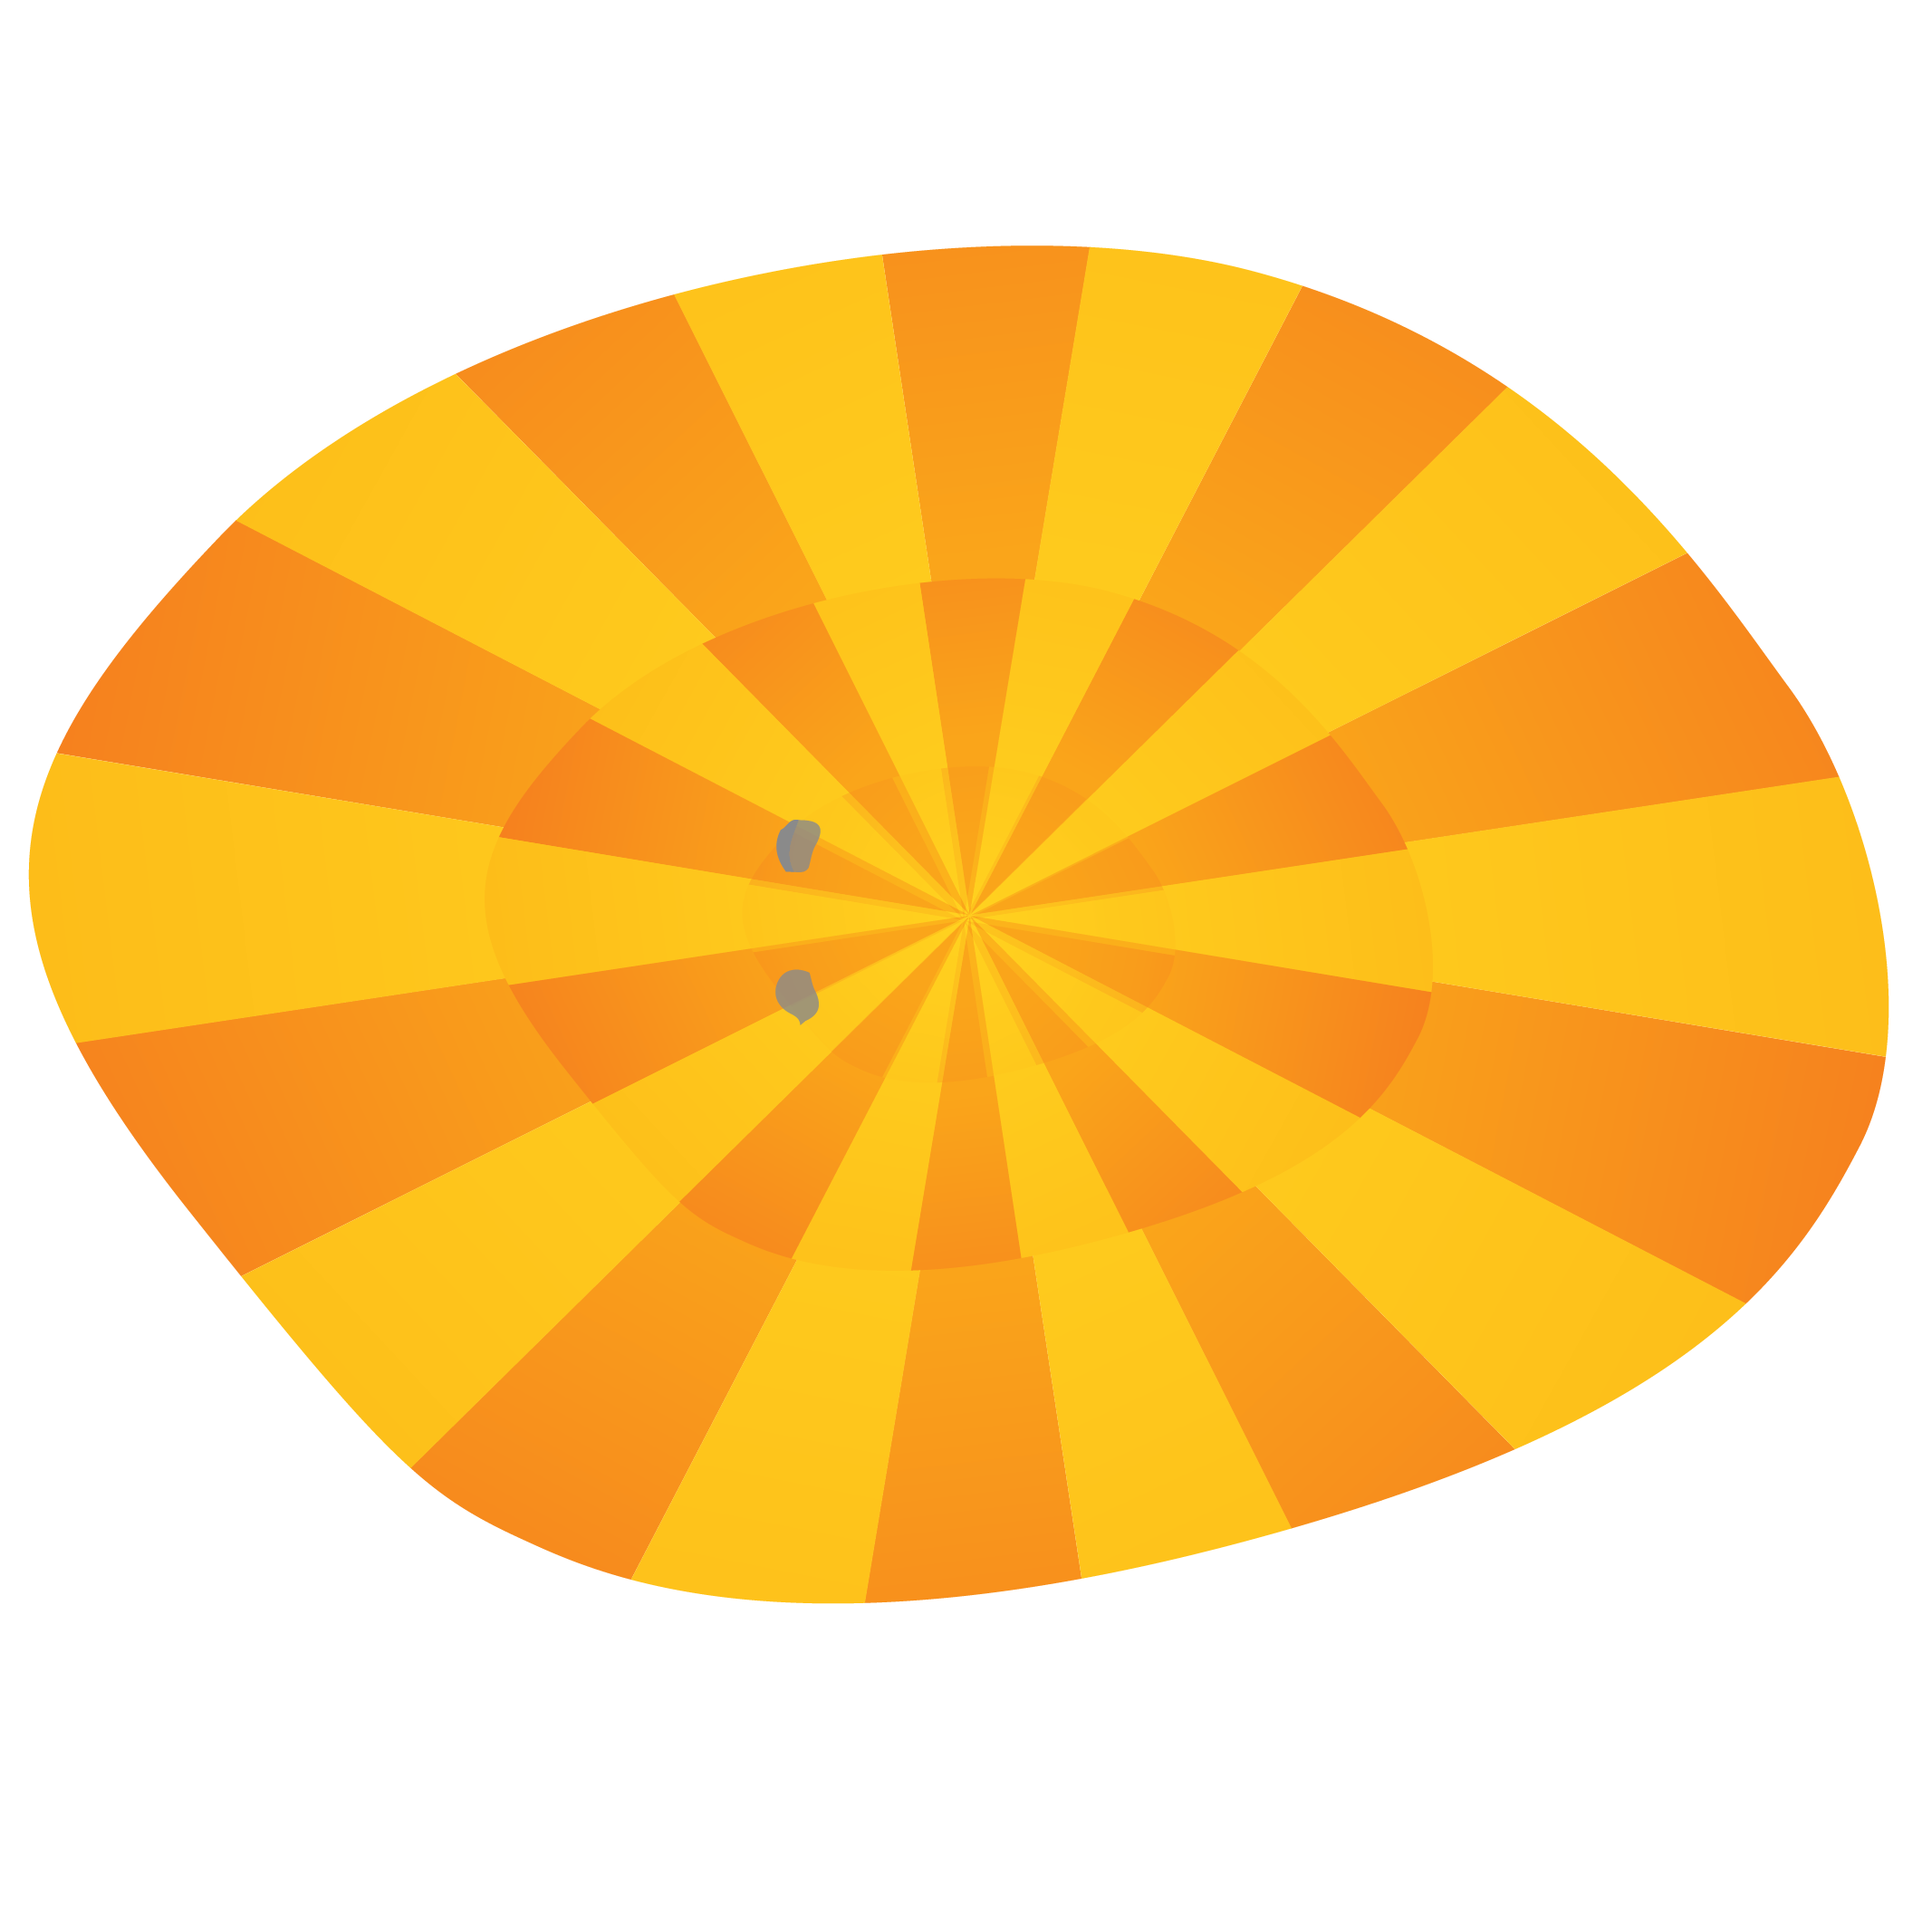
\includegraphics[valign=m,scale=0.1]{images/species_00.png} & Here Comes the Sun & \#imgetendizey & Baby Egg \\ 
Species 1  & 
\includegraphics[valign=m,scale=0.1]{images/species_01.png} & Vampire & Terminator & Batman \\ 
Species 2  & 
\includegraphics[valign=m,scale=0.1]{images/species_02.png} & Little Tongue & Bol & Toad \\ 
Species 3  & 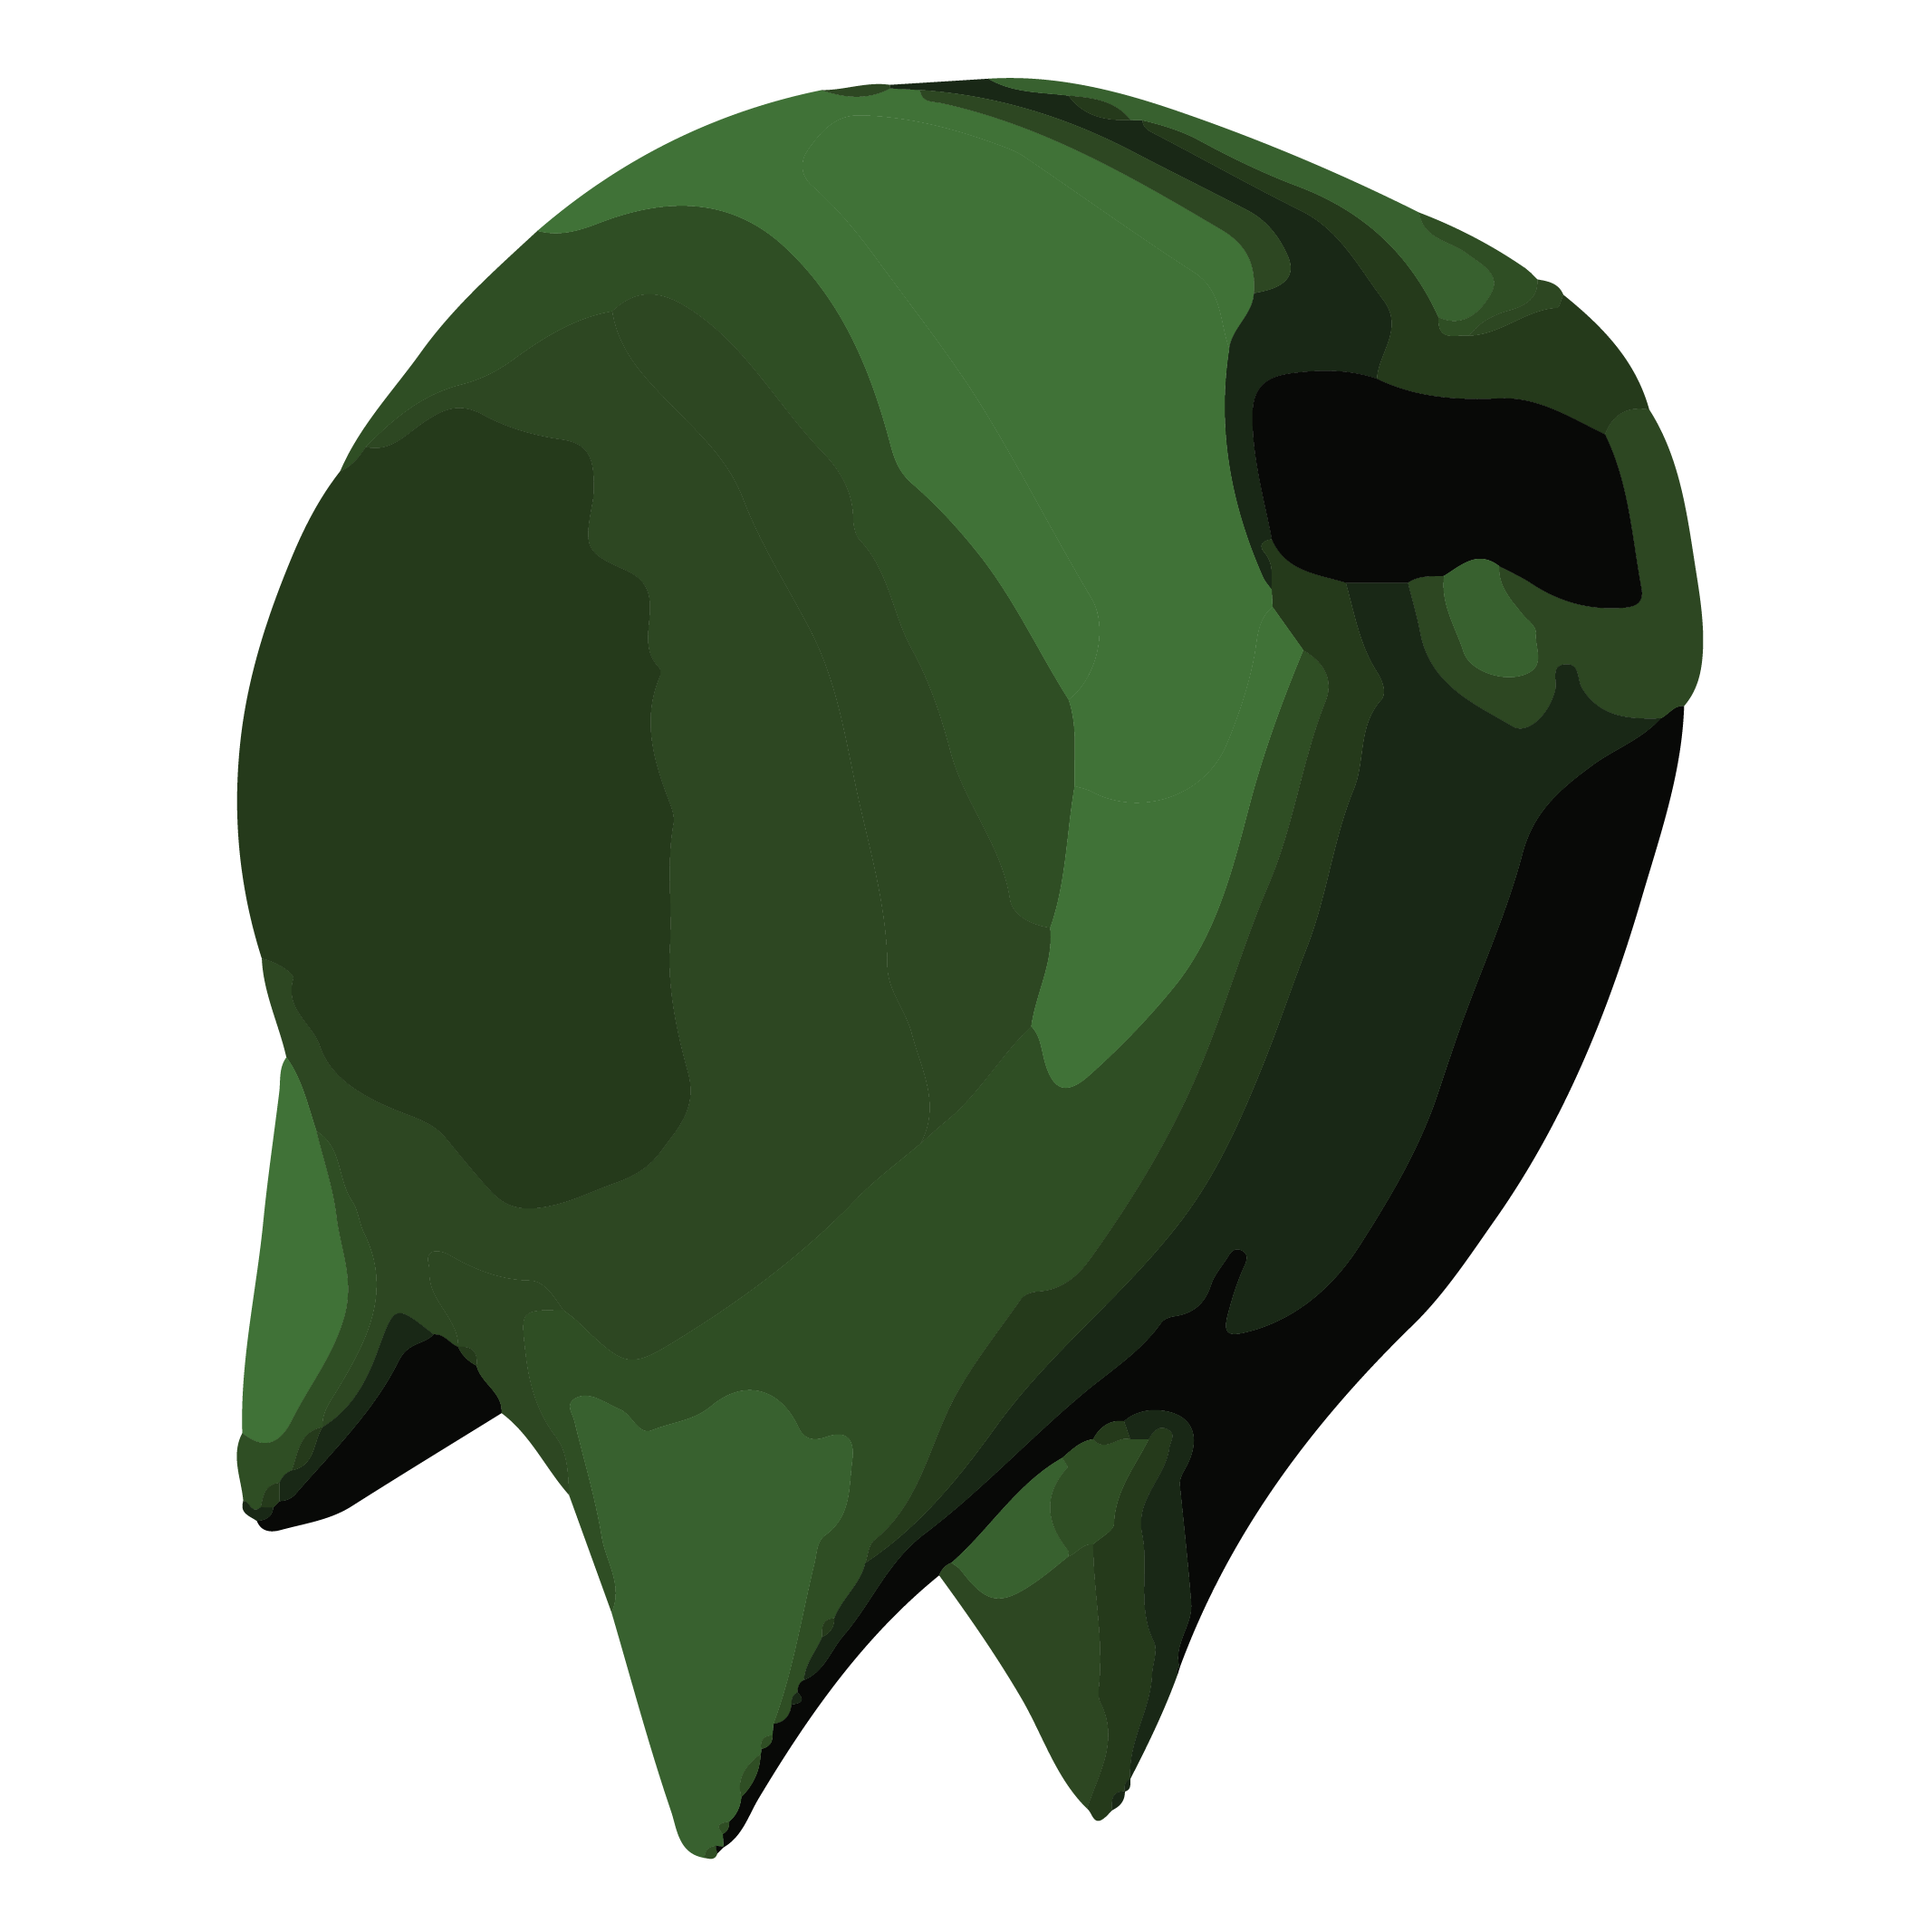
\includegraphics[valign=m,scale=0.1]{images/species_03.png} & Grenngranate & Darock & Broc \\ 
Species 4  & 
\includegraphics[valign=m,scale=0.1]{images/species_04.png} & Purpleberry & Purple Cabbage & Sorbet \\ 
Species 5  & 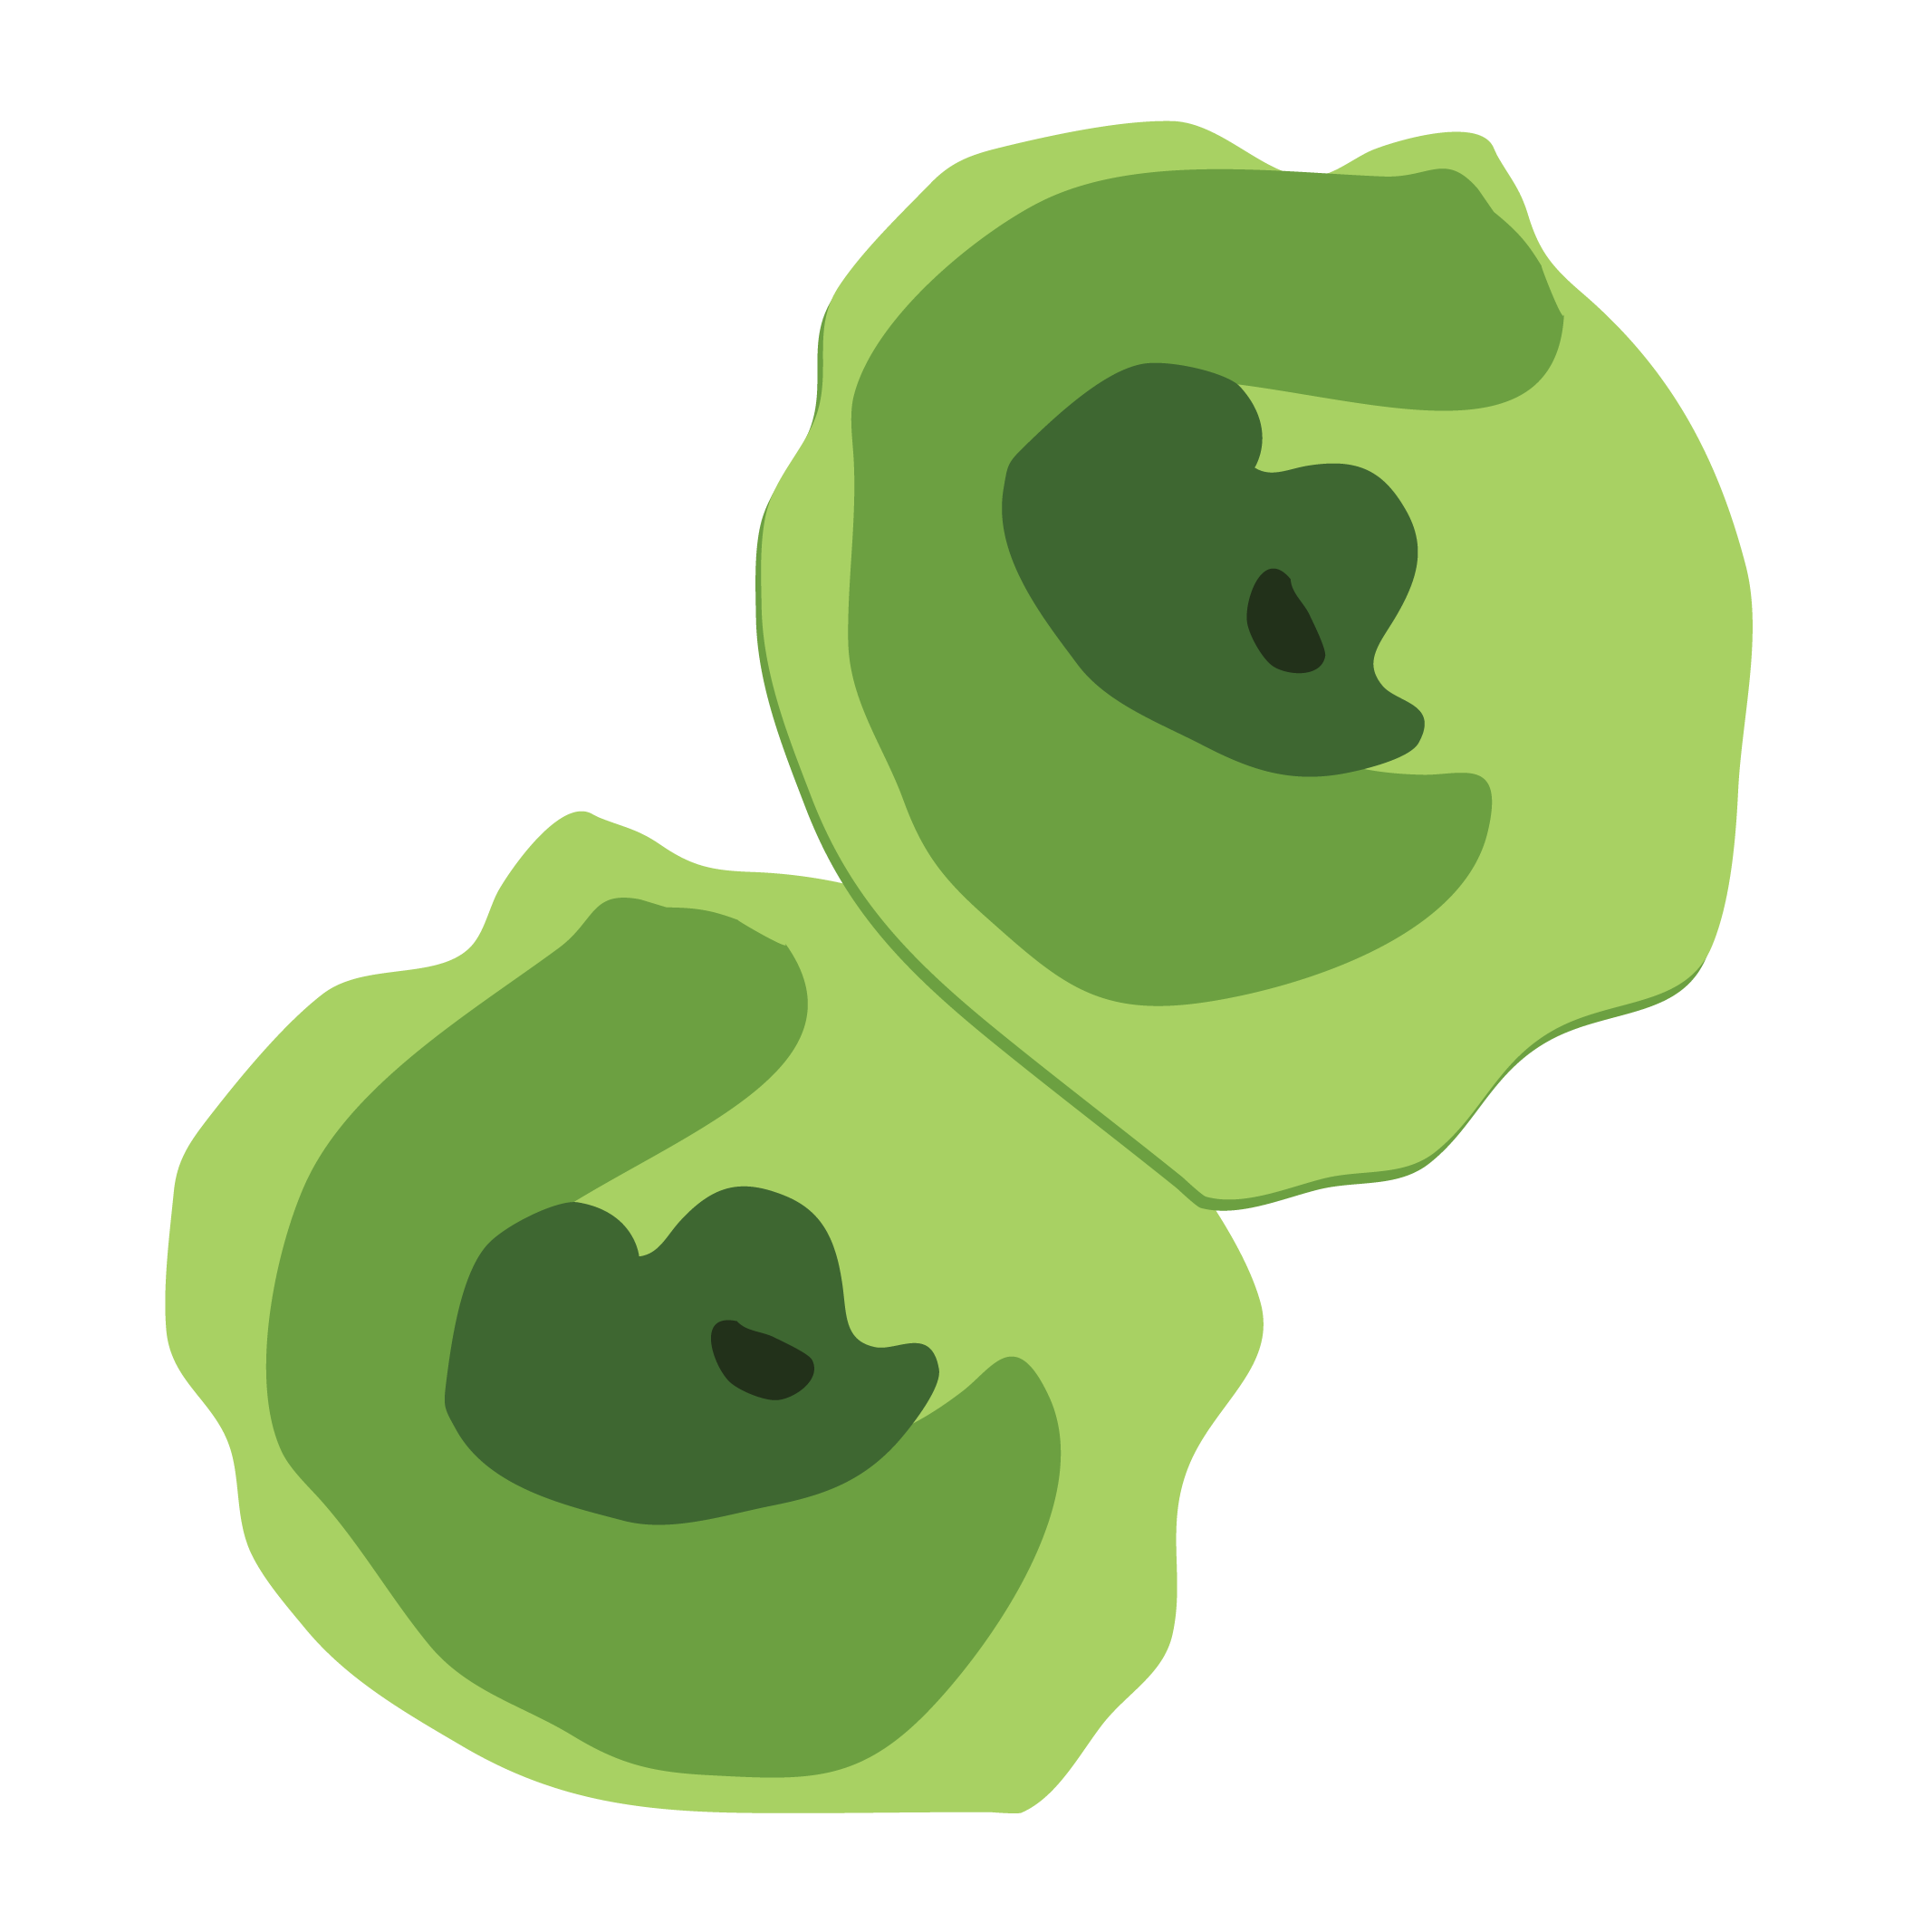
\includegraphics[valign=m,scale=0.1]{images/species_05.png} & Sir Guava & Green Cheecks Busheeks & Peapod \\ 
Species 6  & 
\includegraphics[valign=m,scale=0.1]{images/species_06.png} & Spotted Ninja & SquidWard & Miranda Sings \\ 
Species 7  & 
\includegraphics[valign=m,scale=0.1]{images/species_07.png} & Mello Jello & Sumbraro & Egg \\ 
Species 8  & 
\includegraphics[valign=m,scale=0.1]{images/species_08.png} & Majigger & Miranda Sings & Froggy Thingy \\ 
Species 9  & 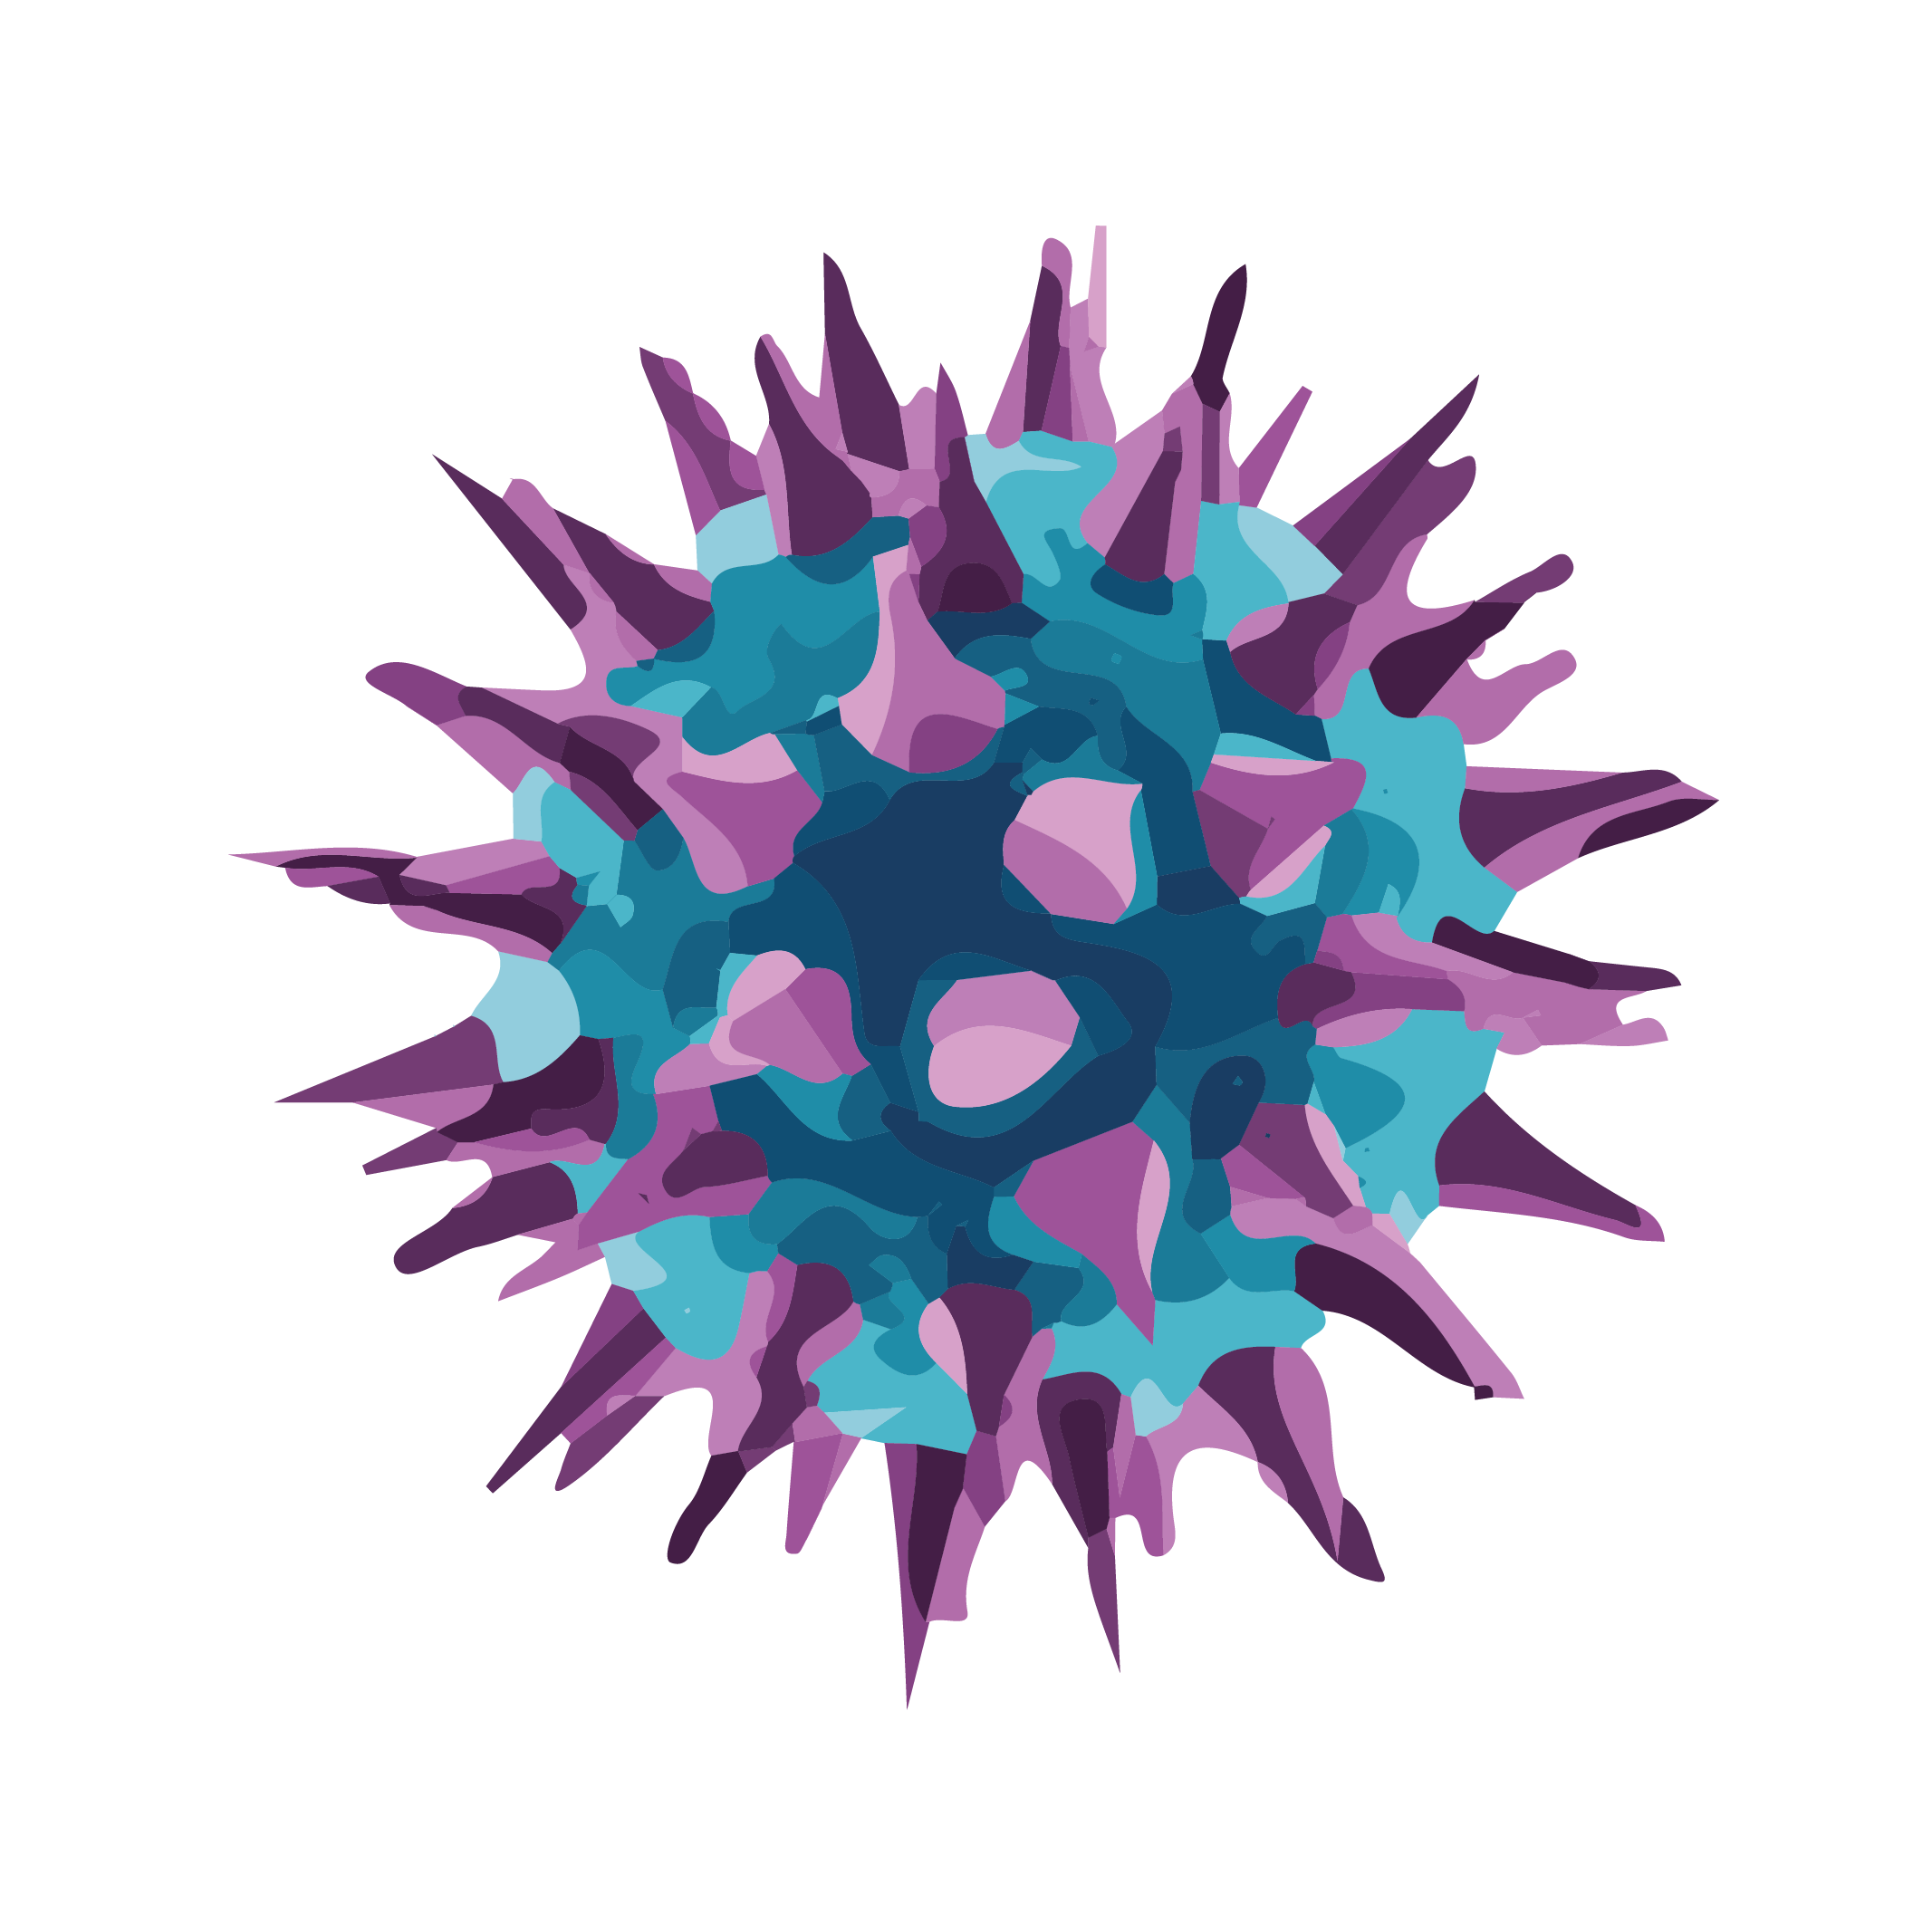
\includegraphics[valign=m,scale=0.1]{images/species_09.png} & Spikeface & Ouch & Spike \\ 
Species 10 & 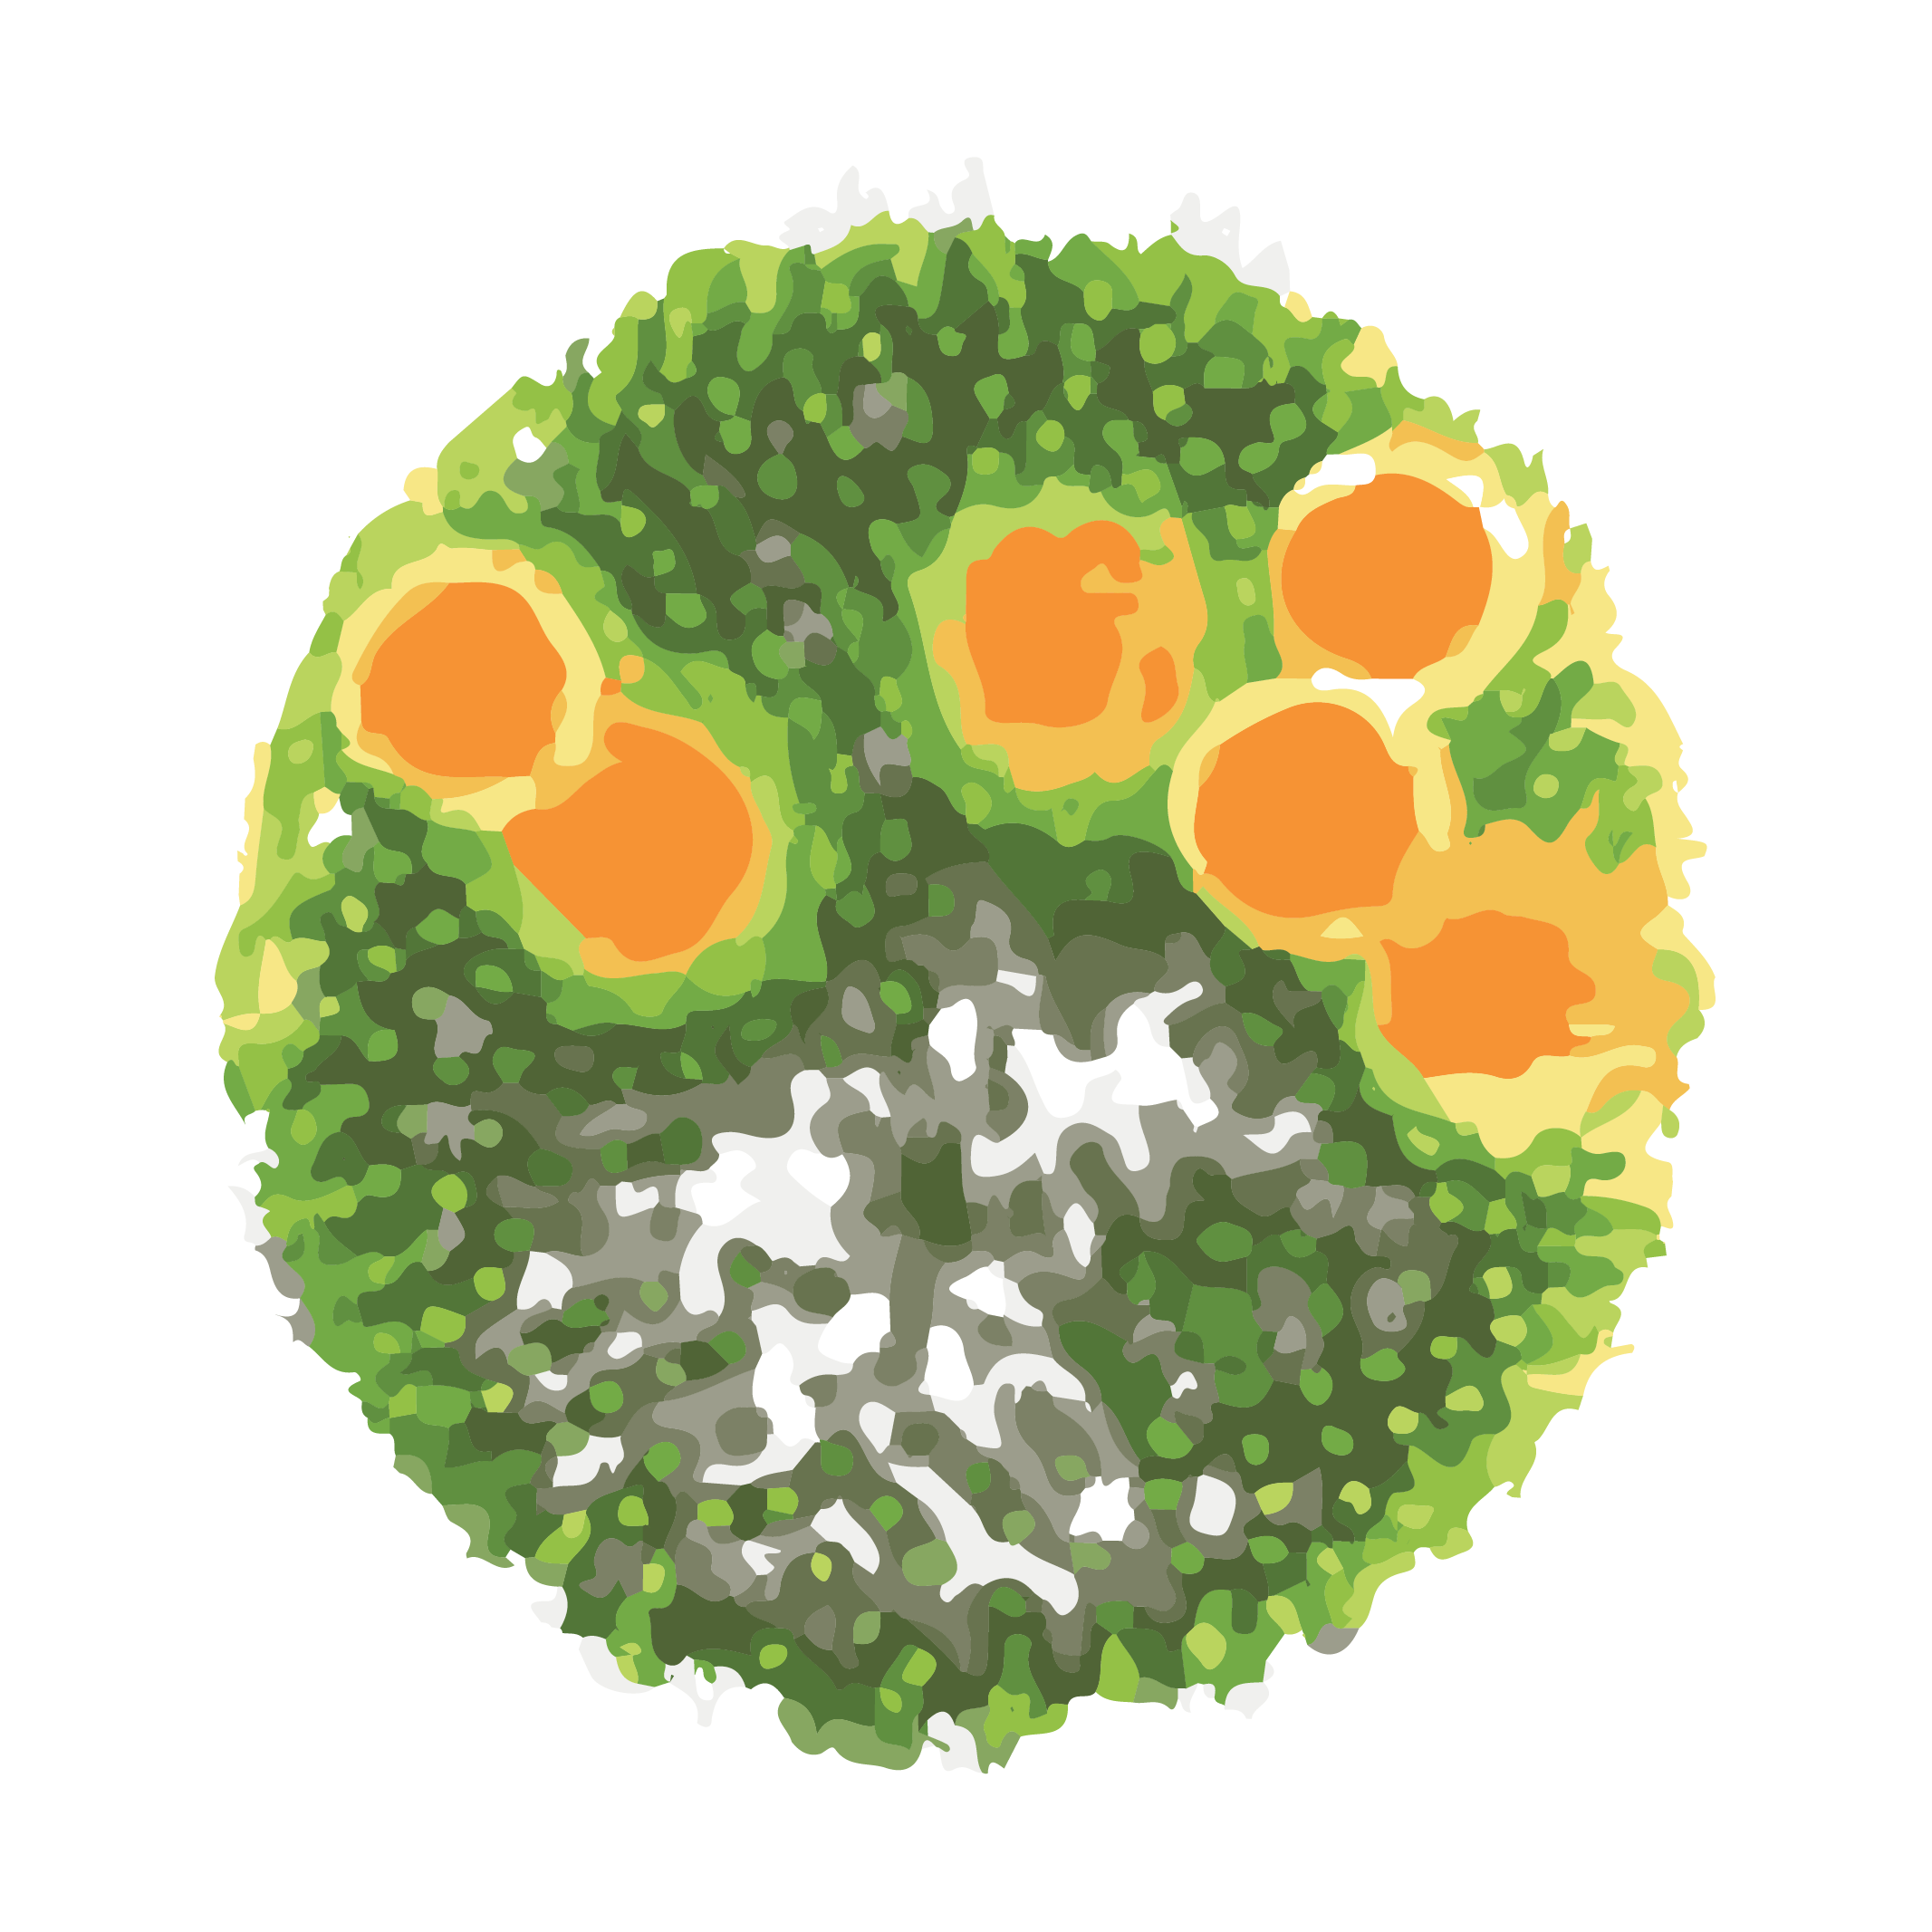
\includegraphics[valign=m,scale=0.1]{images/species_10.png} & Su-Shay & Salad & Chez Bai \\ 
\hline
\end{tabular}
\caption{names assigned by students to creatures}
\label{tab:species_names}
\end{table}

In the questionnaire, 33/46 students preferred this kind of interface over the conventional \textit{Graphical User Interface} (implemented as web interface in this study), despite the fact that using it is more time consuming. 4/46 prefer not to use it, because clicking on a screen is faster and more efficient and the others don't have any preference. In the open questions, the word "fun" was mentioned 42 times (second only to "tangibles" with 57 mentions) and "cool" 20 times. Analyzing the semantics of the explanations, 36 students think that having tangibles is great for creating a fun atmosphere in class and "makes this project even more fun". When asked if they suggest to use the tangibles in the future, 37/46 students answered positively with strong arguments supporting tangibles, 5/46 thought that is better not to use them because they are a waste of time (e.g. waiting in line for others to return them) or because sometimes they had difficulties at the beginning on understanding how to execute an action. An interesting argument (shared by 4 students across all the three classes) is that children don't understand immediately how they works and they are excited and curious about what happens behind the scenes.
\begin{quote}
\textit{[Questionnaire]
I think the tangibles are a good way to get kids excited about learning, since they seem like magic, even though I know that there is a chip of some sort in them.}
\end{quote}
From video sources it is possible to understand that many children were also interested to the technology that make them work because they never saw something similar before. An example that I want to report is a student that placed his hand on top of the iPad in order to see what outcome the system will produce, waiting for few seconds and asking why his hand was not tracked like a tangible. Tools like this can be used in order to make children engaged with general science and develop an interest in computer science.
\begin{quote}
\textit{[Questionnaire]
Use the tangibles because kids will think something like "wow it's magic"}
\end{quote}

Lastly I would like to report that students really appreciated the quality of the tangibles that are a high fidelity reproduction of creatures contained in the computer graphic simulation. Most of them looked at all the creatures’ details before even start using them for the classroom activity.
\begin{quote}
\textit{[Questionnaire]
The tangibles teach us the looks of the creatures because I had no idea what the underside of the creatures.}
\end{quote}
Students were truly inspired by their look and feel, other than expressing verbally their comments they wanted to write them down in the questionnaire:
\begin{quote}
\textit{[Questionnaire]
[...] not only is it lots more fun and interesting, it shows just what a 3-D printer can do!}
\end{quote}

\begin{quote}
\textit{[Questionnaire]
[I like] the tangibles because it's very creative}
\end{quote}

The answer to the first part of the \textit{second research question} is that tangibles can motivate students. During this study, as explained in this section, I found evidence that keeping students engaged into fun and enjoyable activities adds motivational value for the students. 

Collected data also suggest that tangibles have properties of \textit{cultural artifacts} \cite{horn:role}:
\begin{itemize}
\item They activate social resources learned way before starting using them: how to share a toy with other children.
\item Peers taught each other strategies to use them taking advantage of their social skills.
\end{itemize}
The model used for introducing species into habitats (get tangibles close to computer where the habitat is simulated) was not immediately recognized and for this reason they are not \textit{social signifiers} \cite{norman:way}. For this reason I argue that tangibles in this case are not cultural artifacts (even if they present some properties of them). This is the answer to the last part of the second \textit{research question} and gives also a clue on how to better improve tangible interaction in the future for taking full advantage of \textit{cultural artifacts} \cite{horn:role} capabilities that comes with them. 

\subsection{How one set of tangibles helps students to discuss}
Evidence in the video suggest that introducing limited resources (one set of tangibles) that must be used by all the groups creates great opportunities for discussion about the scientific topic of the lecture between children of the same group and also between children in different groups.

This is a behavior that I expected when I described the opportunities that tangibles creates and is the answer the second part of the \textit{second research question}. In this subsection I describe it in details. It was easy to anticipate this behavior, because forcing children to have limited resources naturally creates a place where they have to wait for them to became available.

Perturbation to the habitats, the only activity that required tangibles, was often executed as last activity of the lesson in 15 or 20 minutes of time. Before perturb the habitat every group had to make a proposal and a prediction of the outcome. After the proposal they had to go in the middle of the room, take the tangibles and return to their habitat for executing the action placing the tangible near the iPad. If the tangibles were not available the adopted solutions were two:
\begin{itemize}
\item Go to the the group that owned the needed tangible and ask the permission to be the next to use it.
\item Remain at the central table and discuss with the other students while waiting the desired tangible to became free.
\end{itemize}
Usually for every group only two or three students went to the central table for taking the tangibles, it was rare that the entire group did it.

Students of that classes never used a tangible interface before, this fact encouraged at the beginning discourses on how to use them more than productive didactic discourses. Not every one understood how they works (e.g. they must be placed near the habitat) and they sought the help of classmates. Passed the first lesson discourses became more productive almost exclusively about the action that they wanted to perform on their environment. In the questionnaire 14/46 students admitted to have at least one productive discourse with other groups confirming video evidence:
\begin{quote}
\textit{[Questionnaire]
We mostly talked about what was going on in our ecosystems but we asked some of the other groups what changes they were making.}
\end{quote}

Another positive, interesting and unattended behavior is that students could hear other groups conversations since they were concentrated around the same table, also without a direct interaction:
\begin{quote}
\textit{[Questionnaire]
We talked about it a little bit [perturbation of our habitat] and heard the other groups plans. We all rushed to get the tangibles though I didn't really get to have a conversation.}
\end{quote}
This is also an evidence that the social protocol used for accessing the data was \textit{First to Take First to Use}. There are no sign of disputes between students. The teacher never had to intervene for stopping inappropriate behaviors.
\begin{quote}
\textit{[Questionnaire]
There was a line and we had to wait for them to check ours before we did it.}
\end{quote}

All the behaviors described were positives and contributed to social interaction, free discussion and knowledge exchange, but 15/46 students perceived having only one set of beacons as a problem often identifying the waste of time as an issue for them.
\begin{quote}
\textit{[Questionnaire]
It took a little more time because some groups needed the same tangible.}
\end{quote}
\begin{quote}
\textit{[Questionnaire]
I think that we should not use tangibles next year because they are unnecessary and waste class time. When you put them on the iPad, there can be a delay and it makes us unable to complete certain things.}
\end{quote}

Another interesting and unexpected fact discovered is that children tend to copy the actions of other groups. As shown in \ref{tab:perturbations} there are cases in which the choice of species is not random, for example in perturbation 3 one class chose only species 8 and 10. Evidence supporting this claim are present also in the questionnaire:
\begin{quote}
\textit{[Questionnaire]
In waiting we had an opportunity to discuss with others ecosystems. Also, without even talking, you could see what other ecosystems were doing with a cursory glance.}
\end{quote}

\begin{table}
\centering
\begin{tabular}{ | l | l | l | l | l | l | }
\hline
Perturbation \# & Class  & Habitat \# & Action & Species & Interface \\
\hline
\hline
\multirow{12}{*}{Perturbation 2} & \multirow{4}{*}{6A} & habitat 1 & Decrease  & Species 8 & Web \\
 & & habitat 2 & Increase & Species 8 & Web \\
 & & habitat 3 & Increase & Species 1 \& 2 & Web \\
 & & habitat 4 & Increase & Species 7 & Web \\
\cline{2-6}
 & \multirow{4}{*}{6B} & habitat 1 & Increase & Species 10 & Web \\
 & & habitat 2 & Increase & Species 9 & Web \\
 & & habitat 3 & & & Web \\
 & & habitat 4 & Increase & Species 7 & Web \\
\cline{2-6}
 & \multirow{4}{*}{6C} & habitat 1 & Decrease & Species 10 & Tangible \\
 & & habitat 2 & Increase & Species 0 & Tangible \\
 & & habitat 3 & Increase & Species 1 & Tangible \\
 & & habitat 4 & Decrease & Species 7 & Tangible \\ 
\hline
\multirow{12}{*}{Perturbation 3} & \multirow{4}{*}{6A} & habitat 1 & Decrease & Species 2 & Tangible \\
 & & habitat 2 & Increase & Species 7  & Tangible \\
 & & habitat 3 & Increase & Species 10 & Tangible \\
 & & habitat 4 & Decrease & Species 10 & Tangible \\
\cline{2-6}
 & \multirow{4}{*}{6B} & habitat 1 & Decrease & Species 8 & Tangible* \\
 & & habitat 2 & Decrease & Species 8  & Tangible* \\
 & & habitat 3 & Decrease & Species 10 & Tangible* \\
 & & habitat 4 & Decrease & Species 10 & Tangible* \\
\cline{2-6}
 & \multirow{4}{*}{6C} & habitat 1 & Decrease & Species 8 & Tangible \\
 & & habitat 2 & Increase & Species 7 & Tangible \\
 & & habitat 3 & Increase & Species 3 & Tangible \\
 & & habitat 4 & Decrease & Species 7 & Tangible \\ 
\hline
\multirow{12}{*}{Perturbation 4} & \multirow{4}{*}{6A} & habitat 1 & Insert & Species 7 & Tangible \\
 & & habitat 2 & Insert & Species 1 & Tangible \\
 & & habitat 3 & Insert & Species 0 & Tangible \\
 & & habitat 4 & Insert & Species 1 & Tangible \\
\cline{2-6}
 & \multirow{4}{*}{6B} & habitat 1 & Insert & Species 7 & Tangible \\
 & & habitat 2 & Remove & Species 4 & Tangible \\
 & & habitat 3 & Insert & Species 7 & Tangible \\
 & & habitat 4 & Insert & Species 1 & Tangible \\ 
\cline{2-6}
 & \multirow{4}{*}{6C} & habitat 1 & Remove & Species 8 & Tangible \\
 & & habitat 2 & Remove & Species 9 & Tangible \\
 & & habitat 3 & Insert & Species 2 & Tangible \\
 & & habitat 4 & Insert & Species 9 & Tangible \\ 
\hline
\end{tabular}
\caption{perturbations applied to habitats}
\label{tab:perturbations}
\end{table}

From this story I can gather the answer for the second part of the \textit{second research question}: creating a bottleneck at the central table (where everyone have to take the tangibles) creates an unique place inside the classroom where students can exchange information while waiting and lead to productive discourses about the scientific topic.

\subsection{Feeling more in control and minimize the errors}
I found evidence that children feels more in control of the changes when they use tangibles. In WallCology application the changes applied to ecosystems are extremely important for the outcome of the experiment and students were totally aware of it. Introducing a new species or removing an existing one can have devastating consequences on the populations living in the habitats. For this reason the interface that allow them to modify critical parameters must be designed keeping in mind the error minimization principle \cite{norman:design}. The web interface implements this principle displaying a message asking for a confirmation before applying any change, nevertheless young students didn't feel enough in control because they perceive the affordance \cite{norman:affordance} of irreparably destroy their ecosystem with two clicks (one on the action and one on the confirm button). Tangibles expose a different set of properties that minimize the error possibility requiring locomotion in order to apply changes to the habitat. The evidence can be found in the questionnaire:
\begin{quote}
\textit{[Questionnaire]
I like having tangibles because I think it's easier to focus and concentrate when I'm in control of what I'm doing. [...]}
\end{quote}

\begin{quote}
\textit{[Questionnaire]
I think that it's pretty cool to have tangibles, because whereas the computer is doing everything, you feel like you have more control of your habitat while placing the tangibles on the iPad. I feel this because it's nice to see a practical demonstration of what's going to happen; Chez Ball decreases, Sorbet increases, etc. [...]}
\end{quote}

\begin{quote}
\textit{[Questionnaire]
Because it's easier to visually see what you're actually doing [while using tangibles] and you can't accidentally click the wrong thing.}
\end{quote}

Evidence of mistakes committed by students while using the web interface for executing the second perturbation are present in the application log. Two groups wrongly executed two actions instead of one and one group didn't complete the action the first day (\ref{tab:perturbations}). Group three in 6A increased both species 2 and species 1 and group four increased twice species 7. This kind of errors were not present while they were using the tangible interface because only one modification every 30 seconds was allowed by the interface.

Based on the error evidence other two mechanisms were designed and implemented for improving the usability of the \textit{population control} interface:
\begin{itemize}
\item \textit{Backend input verification system}: it didn't allow more than one consecutive action of the same type on the same species for the same habitat. An error message is also sent to the front end in case the rule is violated (the interaction is logged anyway).
\item \textit{Action executed with success message}: in order to give feedback \cite{norman:design} to the user and be sure that the system successfully register the changes.
\end{itemize}

At this point I listed the evidence necessary to answer the \textit{first research question} and explain how teachers and learners coordinate their use of shared tangibles in this study. Tangibles were left on the central table without any form of control imposed by teachers. Students of all the three classes were able to coordinate the access to the tangibles without problems, following the social protocol \textit{First to Take First to Use} that creates a line and some minutes of waiting time at the central table. Some students decided not to wait in line and went directly to other groups in order to ask the needed tangible, missing the opportunity to discuss with other students, but discovering the perturbation that the other group was applying.

\section{Summary and research results}

It is difficult to assert if tangibles help students to learn, but I found evidence of behaviors that are commonly considered good practice for learning inside the school. Those behaviors are summarized in:
\begin{itemize}
\item Engage the students in fun and glad activities.
\item Inspire curiosity and creativity.
\item Face to face conversations and talks about a scientific inquiry.
\item Discussions and information sharing between different groups while waiting their turn of using tangibles.
\item Know what other groups are doing.
\item Empathy with the creatures and a more personal connection with them.
\end{itemize}

In this study the students were left without teacher control. They were able to autonomously coordinates in order to use the tangibles to accomplish the assigned goal of applying perturbations to the ecosystems. As a result, interactions between students increased in number and were not only focused on the material actions for achieving the goal, but were also about the science domain behind the simulation. Shared control tangibles definitely create opportunities for engaging students in discussions, not possible with classical user interfaces (answer to the second research question of this study). Those discussions were possible because of the competition for having those limited resources and they created no disputes between students. The outcome of this study is overall positive and provides evidence that tangible interfaces are mature enough for being employed in real classes. 

The obtained results also confirms that \textit{RoomPlaces} is able to support those activities making it an essential tool in this research and highlighting its effectiveness in a real use case scenario. \textit{RoomPlaces} was robust enough for supporting 60 uninterrupted days of running concurrently in three different classes without any crash of its components and it required no external intervention for fixing errors during the study (thanks also to the previous six months of lab testing). It was used by researchers other than me that received no training on how to use it other than simple high level instructions that can be easily executed by teachers with no specific competences. During the study, many functions of \textit{RoomPlaces} were not required leaving some open question about their effectiveness and robustness in real case scenarios.

\chapter{Conclusion and Future Work}

\label {ch:conclusions}

\section{Summary}
This thesis presents RoomPlaces: a software framework for supporting science inquiry in the Classroom of Things. In the first chapter I inserted the system in the current context of research, motivating the introduction of location services and tangible interaction interfaces inside classrooms, explaining the opportunities available and not yet explored. Some of those opportunities are inspired by systems built in the last decade found in literature. Every system is very specific for the kind of the teaching application where it is used and there's no common ground in term of employed technologies and code reusing between research groups. The result is that indoor location tracking for learning technologies is still far for being mature and I believe that the first step toward its massive usage is creating a general, reusable tracking system, able to locate both users and tangible objects inside classrooms. In the second chapter I described all the systems that take advantage of the location of objects and users as a computer interface for inserting input into scientific inquiries. All the examples in literature were used for outline the specifications for the general tracking system called RoomPlaces. Proximity tracking is the first functionality that needs to be supported in a tracking systems that aim to be used in schools. By design, RoomPlaces establish the position of objects (dynamic resources) using other objects (static resources) as reference point. In the third chapter I explained six months of software engineering work behind the development of the final tool where all the capabilities for supporting the pre-discussed opportunities were implemented. The best way for providing evidence that the tool successfully supports real cases of classroom activities, is to create a meaningful user study with real research questions and answer them using the capabilities of the software. The forth chapter reports the complete user study carried out in two months using RoomPlaces for creating the human-computer interaction through tangible interfaces. After the study, I reported the results, both answering all the pre-discussd research questions and providing evidence that RoomPlaces and nutella allow to create a complete and complex user study like WallCology (that has a duration of months). The great advantage that comes with RoomPlaces is that the software is already tested and stable. As already reported in the previous chapter, RoomPlaces was used only for tracking tangibles inside classrooms, but was designed for tracking also tablets and users with wearable sensors into multiple reference systems (e.g. discrete and continuous coordinates system). There are many more opportunities for re-using and improving RoomPlaces in the future, I talk about them in the next section.

\section{Future work}

RoomPlaces is the first step in building a general tracking system that supports all the opportunities in location aware applications that are made possible with the introduction of a tracking system. The proximity tracking system was chosen in this first step because it is simple and powerful enough for taking advantage of the opportunities present in classrooms (and listed in the introduction chapter). The next step for continuing the development of RoomPlaces is the integration of more tracking technologies inside the tracking layer. This integration will be possible because of the abstraction layer (RoomPlaces APIs) that completely separates the technology of the tracking system and system calls that are available for the high level application development. Among the other possibilities there are the triangulation and trilateration based technologies that can take advantage of radio and ultrasound signals. These technologies will enable more accurate location of users and objects inside the room and will allow to create applications that require great precision for working, for example augmented reality systems where a virtual layer (based on the location of certain objects) is overlapped to the physical world.

Another interesting future work is scaling the capabilities of RoomPlaces in order to support many more users, objects and places tracked than now. In the next paragraph I will describe possible scenarios where those technology can improve the life of people.

With minor iterative improvements is will be possible to use RoomPlaces in multi-room environments, employing indoor location in entire buildings and tracking users moving across different ares. It is easy to see how applications can be built for many fields way beyond learning technologies. In museums and interactive exhibitions there's the opportunity to provide the user with location dependent content on personal devices and also on shared media (like big screens shared among many users). Tracking patients and visitors in hospitals with the goal of providing indoor navigation information is a priority in research \cite{yang:ibeacon}. RoomPlaces could be employed for this kind of applications without the need of building custom solutions. Reliability of the system is essential during indoor navigation, information must be available at the right time for being useful. Smart homes are also an active area of research where RoomPlaces could be employed. Knowing how many people are present in each room can be the key for creating user friendly "smart spaces" where lights, temperature and security are location dependent with the goal of reducing energy consumption and release the user from trivial tasks (e.g. turning on lights, lowering the temperature while outside). An extension of the multi-room tracking system is a city-wide tracking system, where sensors are employed for providing high precision location beyond GPS position (i.e. when high vertical accuracy is required) in specific areas in order to provide services to both users and city infrastructures. Possible applications are fruition of customized content on shared displays (e.g. information about travels of passengers near the display), real-time train scheduling based on people waiting at the stop knowing their destination with the goal of minimize the waiting time during changes.

All the described applications could be supported using RoomPlaces as intermediary layer between the tracking technology and the application. The approach that employ a general tracking system, I think, will be successful for attacking location tracking problems, because the core functions identified in this thesis are common to all those problems. Different systems require different accuracy. For this reason RoomPlaces must be flexible enough for support different tracking methodologies and provide a unified interface that can be employed in many different scenarios. Using a single general system in multiple applications will enable to update it overtime learning from experiences in different fields.



\appendices
\newpage
\appendix

\chapter{Nutella protocol}

\label{apdx:nutella_protocol}

In this appendix I describe how nutella protocol works and how it implements the functionalities requested for providing push and pull strategies.

Nutella protocol encapsulate messages into MQTT protocol that allows binary content. By design nutella protocol allows only content that can be encoded as JSON (basically everything) and add a little payload that allows both end to communicate using the right strategy.

A nutella message looks like this:

\begin{lstlisting}[language=NutellaProtocol]
{
    "id": "req_res_id",
    "from": {
        "type": "run",
        "run_id": "my_run_id",
        "app_id": "my_app_id",
        "component_id": "my_component_id",
        "resource_id": "my_resource_id"
    },
    "type": "request",
    "payload": {
        /* Custom data */
    }
}
\end{lstlisting}

In order to distinguish between push and pull strategy it is used "type" field (the more external one) that can be "request", "response" or "publish".
\begin{itemize}
    \item \textit{Request}: from client to server
    \item \textit{Response}: from server to client
    \item \textit{Publish}: peer communication
\end{itemize}

The custom data in inserted in the "payload" field and is encoded in JSON format.

The "from" field is passed as is to the subscribe and handle request callbacks and it is used mainly for debugging purposes.

This protocol is never seen from the developer because the nutella.net primitives automatically incapsulate and decapsulate the payload automatically when they're called.

The primitives are:
\begin{itemize}
    \item \textit{nutella.net.subscribe(channel, callback(message, from))}
    \item \textit{nutella.net.publish(channel, message)}
    \item \textit{nutella.net.request(channel, request)}
    \item \textit{nutella.net.handle\_requests(channel, callback(request, from))}
\end{itemize}
\chapter{RoomPlaces protocol}

\label{apdx:roomplaces_protocol}


RoomPlaces protocol is a set of rules that allow every RoomPlaces component to communicate. It is specifically designed for supporting the following functionalities:
\begin{itemize}
    \item Add resource
    \item Delete resource
    \item Update the resource position for automatic tracked resources
    \item Update the resource location for static resources
    \item Update the state of the resource (data associated to that resource)
    \item Add, modify and remove a discrete tracking coordinate system
    \item Notify arrival and departure events (when a dynamic resource is near a static resource)
\end{itemize}

The protocol supports also groupings: a group of resources allow more efficient resource retrieval. This functionality was not implemented in the first prototype.

The majority of the functionalities can be accessed in both \textit{push} (subscribing to a channel and wait for update) and \textit{pull} (explicitly requesting the data) modality. The idea behind this choice is that \textit{nutella.location} needs the state of the entire system during the start-up phase and then only small updates for being synchronized with the central server.

In this appendix I describe the RoomPlaces protocol using BNF \cite{naur:revised} for the grammar. This protocol is based on the notion of nutella channels, every channel has also a modality that can be publish/subscribe or request/response (a channel can also support both the modalities because nutella protocol support it \autoref{apdx:nutella_protocol})


\section{Publish/Subscribe channels}
All the channels are padded with \textit{/location} that is the convention name for \textit{nutella.location} communications.

\begin{table}
\centering
\begin{tabular}{ | l | l | l | l | }
    \hline Channel & Description & Recipient & Message \\
    \hline /resource/add                & Add a new resource        & Server & $<$resource\_add$>$ \\
    \hline /resource/remove             & Remove a resource         & Server & $<$resource\_remove$>$ \\
    \hline /resource/update             & Update a resource         & Server & $<$resource\_update$>$ \\
    \hline /resources/update            & Update a set of resources & Server & $<$resources\_update$>$ \\
    \hline /resources/added             & Set of resources added    & Client & $<$resources\_added$>$ \\
    \hline /resources/removed           & Set of resources removed  & Client & $<$resources\_removed$>$ \\
    \hline /resources/updated           & Set of resources updated  & Client & $<$resources\_updated$>$ \\
    \hline /room/update                 & Update the room           & Server & $<$room\_update$>$ \\
    \hline /room/updated                & Notify a room update      & Client & $<$room\_updated$>$ \\
    \hline /resource/static/$<$rid$>$/enter & Notify an enter event & Client & $<$event\_enter$>$ \\
    \hline /resource/static/$<$rid$>$/exit  & Notify an exit event  & Client & $<$event\_exit$>$ \\
    \hline /tracking/discrete/update    & Update the discrete coord & Server & $<$discrete\_update$>$ \\
    \hline /tracking/discrete/updated   & Notify disc coord update  & Client & $<$discrete\_updated$>$ \\
    \hline
\end{tabular}
\end{table}

\section{Request/Response channels}
All the channels are padded with \textit{/location} that is the convention name for \textit{nutella.location} communications.

Every request is done from the clients and the server will send a response. 
\begin{table}
\centering
\begin{tabular}{ | l | l | l | l | }
    \hline Channel & Description & Response \\
    \hline /resources                & Set of resources                 & $<$resources\_response$>$ \\
    \hline /room                     & Room Information                 & $<$room\_response$>$ \\
    \hline /tracking/discrete        & Discrete coordinate information  & $<$discrete\_response$>$ \\
    \hline
\end{tabular}
\end{table}

\section{Protocol grammar}
The RoomPlaces protocol grammar is a subset of JSON grammar because it uses JSON primitives (present in the majority of the programming languages) for "stringifying" objects.

\begin{lstlisting}[language={}]
<resource_add> ::= {"rid": "<rid>", "model": "<model>", "type": "<type>" [, "proximity_range": <float>]}
<resource_remove> ::= {"rid": "<rid>"}
<resource_update> ::= {"rid": "<rid>", (<continuous> | <discrete> | <proximity> | <parameters>)}
<resources_update> ::= {"resources": `[' [<resource_update> (, <resource_update>)* ] `]'}
<resources_added> ::= {"resources": `[' <resource> (, <resource>)* `]'}
<resources_removed> ::= 
<resources_updated> ::= {"rid": "<rid>", "model": "<model>", "type": "<type>", (<continuous> | <discrete> | <proximity>), <parameters_updated> [, "proximity_range": <float>]}
<room_update> ::= {"x": <float>, "y": <float>}
<room_updated> ::= <room_update>
<event_enter> ::= {"resources": `[' <resource> (, <resource>)* `]'}
<event_exit> ::= {"resources": `[' <resource> (, <resource>)* `]'}
<discrete_update> ::= {"tracking": <discrete_tracking>}
<discrete_updated> ::= <discrete_update>

<resources_response> ::= {"resources": `[' <resource> (, <resource>)* `]'}
<room_response> ::= <room_update>
<discrete_response> ::= {tracking: <discrete_tracking>}

<resource> ::= {"rid": "<rid>", "model": "<model>", "type": "<type>"}
<continuous> ::= "continuous": {x: <float>, y: <float>}
<discrete> ::= "discrete": {"x": <discrete_n>, "y": <discrete_n>}
<proximity> ::= "proximity": {["rid": "<rid>", "distance": <float>]}
<parameters> ::= "parameters": `['[<parameter> (, <parameter>)*]`]'
<parameter> ::= {"key": "<string>" , ("value": "<string>" | "delete": true)}
<parameters_updated> ::= "parameters": {(<key>: '<string>')*}
<discrete_tracking> ::= {"x": <float>, "y": <float>, "width": <float>, "height": <float>, "n_x": <float>, "n_y": <float>, "t_x": "<discrete_type>", "t_y": "<discrete_type>"}
<discrete_type> ::= NUMBER | LETTER
<discrete_n> ::= <int> | <uppercase_char>
<key> ::= <string>
<rid> ::= <string>
<int> ::= <digit>+
<string> ::= (<digit> | <uppercase_char> | <lowercase_char>)*
<digit> ::= 0 | 1 | 2 | 3 | 4 | 5 | 6 | 7 | 8 | 9
<uppercase_char> ::= A | B | C | D | E | F | G | H | I | J | K | L | M | N | O | P | Q | R | S | T | U | V | W | X | Y | Z
<lowercase_char> ::= a | b | c | d | e | f | h | h | i | j | k | l | m | n | o | p | q | r | s | t | u | v | w | x | y | z
\end{lstlisting}




\chapter{RoomPlaces APIs}

\label{apdx:roomplaces_api}

In this appendix I describe in details \textit{RoomPlaces} APIs. The goal of this APIs in providing a fast way for accessing \textit{RoomPlaces} functionalities, for this reason they are contained in the nutella library and are accessible though function call in the native language. On this appendix I will explain every function call using a Javascript syntax, in the other languages the conventions of the language are followed.

\section{Obtaining a resource object}

\begin{lstlisting}
nutella.location.resources
\end{lstlisting}
Return an array of resources.

\begin{lstlisting}
nutella.location.resource['rid']
\end{lstlisting}
Retrieve the resource with the specified \textit{rid}.

\section{Resource object manipulation}
Every resource is an instance of an object and properties of the object are the information associated to the resource like position and additional parameters.

\begin{lstlisting}
resource.continuous.x
\end{lstlisting}
Return the x coordinate in the continuous reference system. 

\begin{lstlisting}
resource.continuous.y
\end{lstlisting}
Return the y coordinate in the continuous reference system.

\begin{lstlisting}
resource.discrete.x
\end{lstlisting}
Return the x coordinate in the discrete reference system.

\begin{lstlisting}
resource.discrete.y
\end{lstlisting}
Return the y coordinate in the discrete reference system.

\begin{lstlisting}
resource.proximity.rid
\end{lstlisting}
Property present in dynamic resources automatically tracked with the proximity tracking system. Return the resource identifier of the nearest static resource if the current resource is in the range.

\begin{lstlisting}
resource.proximity.proximity.continuous.x
\end{lstlisting}
Property present in dynamic resources automatically tracked with the proximity tracking system. Return the continuous x coordinate of the nearest static resource if the current resource is in the range.

\begin{lstlisting}
resource.proximity.proximity.continuous.y
\end{lstlisting}
Property present in dynamic resources automatically tracked with the proximity tracking system. Return the continuous y coordinate of the nearest static resource if the current resource is in the range.

\begin{lstlisting}
resource.proximity.proximity.discrete.x
\end{lstlisting}
Property present in dynamic resources automatically tracked with the proximity tracking system. Return the discrete x coordinate of the nearest static resource if the current resource is in the range.

\begin{lstlisting}
resource.proximity.proximity.discrete.y
\end{lstlisting}
Property present in dynamic resources automatically tracked with the proximity tracking system. Return the discrete y coordinate of the nearest static resource if the current resource is in the range.

\section{Tangible containers}

\begin{lstlisting}
resource.parameters
\end{lstlisting}
Return a map of parameters

\begin{lstlisting}
resource.parameter['key']
\end{lstlisting}
Return the value of the parameter identified with "key" name. Writing on the element identified with "key" will overwrite the previous value.

\begin{lstlisting}
resource.notifyUpdate
\end{lstlisting}
Writing true on this property will cause a notification function callback to be fired every time the resource is updated in any part of the system.

\begin{lstlisting}
resource.notifyEnter
\end{lstlisting}
This can be set to true only on static resources. Writing true on this property will cause a notification function callback to be fired every time a dynamic resource enter in the range. It will not be fired for resources that are already in the range when the system start, use the \textit{pull} API for this.

\begin{lstlisting}
resource.notifyExit
\end{lstlisting}
This can be set to true only on static resources. Writing true on this property will cause a notification function callback to be fired every time a dynamic resource enter in the range.

\begin{lstlisting}
nutella.location.resourceUpdated(function(resource) {
    /* callback code here */
})
\end{lstlisting}
Called when a resource is updated only for the resources that have \textit{resource.notifyUpdate = true}. 

\begin{lstlisting}
nutella.location.resourceEntered(function(dynamicResource, staticResource) {
    /* callback code here */
})
\end{lstlisting}
Called when a dynamic resource enter in the range of a static resource only for the resources that have \textit{resource.notifyEnter = true}.

\begin{lstlisting}
nutella.location.resourceExited(function(dynamicResource, staticResource) {
    /* callback code here */
})
\end{lstlisting}
Called when a dynamic resource enter in the range of a static resource only for the resources that have \textit{resource.notifyExit = true}.

\begin{lstlisting}
nutella.location.ready(function() {
    /* callback code here */
})
\end{lstlisting}
Called only once when the RoomPlaces APIs are synchronized with the remote state of the server and ready to be used. Every call done before this callback is fired will not work properly and will return an inconsistent state. 


\nocite{*}
\bibformb
\bibliography{uicbib}

\newpage
\vita
\begin{singlespace}
\LTXtable{\textwidth}{chapters/07_Vita.tex}
\end{singlespace}

\end{document}
